% Options for packages loaded elsewhere
\PassOptionsToPackage{unicode}{hyperref}
\PassOptionsToPackage{hyphens}{url}
\PassOptionsToPackage{dvipsnames,svgnames,x11names}{xcolor}
%
\documentclass[
  letterpaper,
  DIV=11,
  numbers=noendperiod]{scrartcl}

\usepackage{amsmath,amssymb}
\usepackage{iftex}
\ifPDFTeX
  \usepackage[T1]{fontenc}
  \usepackage[utf8]{inputenc}
  \usepackage{textcomp} % provide euro and other symbols
\else % if luatex or xetex
  \usepackage{unicode-math}
  \defaultfontfeatures{Scale=MatchLowercase}
  \defaultfontfeatures[\rmfamily]{Ligatures=TeX,Scale=1}
\fi
\usepackage{lmodern}
\ifPDFTeX\else  
    % xetex/luatex font selection
\fi
% Use upquote if available, for straight quotes in verbatim environments
\IfFileExists{upquote.sty}{\usepackage{upquote}}{}
\IfFileExists{microtype.sty}{% use microtype if available
  \usepackage[]{microtype}
  \UseMicrotypeSet[protrusion]{basicmath} % disable protrusion for tt fonts
}{}
\makeatletter
\@ifundefined{KOMAClassName}{% if non-KOMA class
  \IfFileExists{parskip.sty}{%
    \usepackage{parskip}
  }{% else
    \setlength{\parindent}{0pt}
    \setlength{\parskip}{6pt plus 2pt minus 1pt}}
}{% if KOMA class
  \KOMAoptions{parskip=half}}
\makeatother
\usepackage{xcolor}
\setlength{\emergencystretch}{3em} % prevent overfull lines
\setcounter{secnumdepth}{-\maxdimen} % remove section numbering
% Make \paragraph and \subparagraph free-standing
\makeatletter
\ifx\paragraph\undefined\else
  \let\oldparagraph\paragraph
  \renewcommand{\paragraph}{
    \@ifstar
      \xxxParagraphStar
      \xxxParagraphNoStar
  }
  \newcommand{\xxxParagraphStar}[1]{\oldparagraph*{#1}\mbox{}}
  \newcommand{\xxxParagraphNoStar}[1]{\oldparagraph{#1}\mbox{}}
\fi
\ifx\subparagraph\undefined\else
  \let\oldsubparagraph\subparagraph
  \renewcommand{\subparagraph}{
    \@ifstar
      \xxxSubParagraphStar
      \xxxSubParagraphNoStar
  }
  \newcommand{\xxxSubParagraphStar}[1]{\oldsubparagraph*{#1}\mbox{}}
  \newcommand{\xxxSubParagraphNoStar}[1]{\oldsubparagraph{#1}\mbox{}}
\fi
\makeatother

\usepackage{color}
\usepackage{fancyvrb}
\newcommand{\VerbBar}{|}
\newcommand{\VERB}{\Verb[commandchars=\\\{\}]}
\DefineVerbatimEnvironment{Highlighting}{Verbatim}{commandchars=\\\{\}}
% Add ',fontsize=\small' for more characters per line
\usepackage{framed}
\definecolor{shadecolor}{RGB}{241,243,245}
\newenvironment{Shaded}{\begin{snugshade}}{\end{snugshade}}
\newcommand{\AlertTok}[1]{\textcolor[rgb]{0.68,0.00,0.00}{#1}}
\newcommand{\AnnotationTok}[1]{\textcolor[rgb]{0.37,0.37,0.37}{#1}}
\newcommand{\AttributeTok}[1]{\textcolor[rgb]{0.40,0.45,0.13}{#1}}
\newcommand{\BaseNTok}[1]{\textcolor[rgb]{0.68,0.00,0.00}{#1}}
\newcommand{\BuiltInTok}[1]{\textcolor[rgb]{0.00,0.23,0.31}{#1}}
\newcommand{\CharTok}[1]{\textcolor[rgb]{0.13,0.47,0.30}{#1}}
\newcommand{\CommentTok}[1]{\textcolor[rgb]{0.37,0.37,0.37}{#1}}
\newcommand{\CommentVarTok}[1]{\textcolor[rgb]{0.37,0.37,0.37}{\textit{#1}}}
\newcommand{\ConstantTok}[1]{\textcolor[rgb]{0.56,0.35,0.01}{#1}}
\newcommand{\ControlFlowTok}[1]{\textcolor[rgb]{0.00,0.23,0.31}{\textbf{#1}}}
\newcommand{\DataTypeTok}[1]{\textcolor[rgb]{0.68,0.00,0.00}{#1}}
\newcommand{\DecValTok}[1]{\textcolor[rgb]{0.68,0.00,0.00}{#1}}
\newcommand{\DocumentationTok}[1]{\textcolor[rgb]{0.37,0.37,0.37}{\textit{#1}}}
\newcommand{\ErrorTok}[1]{\textcolor[rgb]{0.68,0.00,0.00}{#1}}
\newcommand{\ExtensionTok}[1]{\textcolor[rgb]{0.00,0.23,0.31}{#1}}
\newcommand{\FloatTok}[1]{\textcolor[rgb]{0.68,0.00,0.00}{#1}}
\newcommand{\FunctionTok}[1]{\textcolor[rgb]{0.28,0.35,0.67}{#1}}
\newcommand{\ImportTok}[1]{\textcolor[rgb]{0.00,0.46,0.62}{#1}}
\newcommand{\InformationTok}[1]{\textcolor[rgb]{0.37,0.37,0.37}{#1}}
\newcommand{\KeywordTok}[1]{\textcolor[rgb]{0.00,0.23,0.31}{\textbf{#1}}}
\newcommand{\NormalTok}[1]{\textcolor[rgb]{0.00,0.23,0.31}{#1}}
\newcommand{\OperatorTok}[1]{\textcolor[rgb]{0.37,0.37,0.37}{#1}}
\newcommand{\OtherTok}[1]{\textcolor[rgb]{0.00,0.23,0.31}{#1}}
\newcommand{\PreprocessorTok}[1]{\textcolor[rgb]{0.68,0.00,0.00}{#1}}
\newcommand{\RegionMarkerTok}[1]{\textcolor[rgb]{0.00,0.23,0.31}{#1}}
\newcommand{\SpecialCharTok}[1]{\textcolor[rgb]{0.37,0.37,0.37}{#1}}
\newcommand{\SpecialStringTok}[1]{\textcolor[rgb]{0.13,0.47,0.30}{#1}}
\newcommand{\StringTok}[1]{\textcolor[rgb]{0.13,0.47,0.30}{#1}}
\newcommand{\VariableTok}[1]{\textcolor[rgb]{0.07,0.07,0.07}{#1}}
\newcommand{\VerbatimStringTok}[1]{\textcolor[rgb]{0.13,0.47,0.30}{#1}}
\newcommand{\WarningTok}[1]{\textcolor[rgb]{0.37,0.37,0.37}{\textit{#1}}}

\providecommand{\tightlist}{%
  \setlength{\itemsep}{0pt}\setlength{\parskip}{0pt}}\usepackage{longtable,booktabs,array}
\usepackage{calc} % for calculating minipage widths
% Correct order of tables after \paragraph or \subparagraph
\usepackage{etoolbox}
\makeatletter
\patchcmd\longtable{\par}{\if@noskipsec\mbox{}\fi\par}{}{}
\makeatother
% Allow footnotes in longtable head/foot
\IfFileExists{footnotehyper.sty}{\usepackage{footnotehyper}}{\usepackage{footnote}}
\makesavenoteenv{longtable}
\usepackage{graphicx}
\makeatletter
\def\maxwidth{\ifdim\Gin@nat@width>\linewidth\linewidth\else\Gin@nat@width\fi}
\def\maxheight{\ifdim\Gin@nat@height>\textheight\textheight\else\Gin@nat@height\fi}
\makeatother
% Scale images if necessary, so that they will not overflow the page
% margins by default, and it is still possible to overwrite the defaults
% using explicit options in \includegraphics[width, height, ...]{}
\setkeys{Gin}{width=\maxwidth,height=\maxheight,keepaspectratio}
% Set default figure placement to htbp
\makeatletter
\def\fps@figure{htbp}
\makeatother

\usepackage{booktabs}
\usepackage{caption}
\usepackage{longtable}
\usepackage{colortbl}
\usepackage{array}
\KOMAoption{captions}{tableheading}
\makeatletter
\@ifpackageloaded{tcolorbox}{}{\usepackage[skins,breakable]{tcolorbox}}
\@ifpackageloaded{fontawesome5}{}{\usepackage{fontawesome5}}
\definecolor{quarto-callout-color}{HTML}{909090}
\definecolor{quarto-callout-note-color}{HTML}{0758E5}
\definecolor{quarto-callout-important-color}{HTML}{CC1914}
\definecolor{quarto-callout-warning-color}{HTML}{EB9113}
\definecolor{quarto-callout-tip-color}{HTML}{00A047}
\definecolor{quarto-callout-caution-color}{HTML}{FC5300}
\definecolor{quarto-callout-color-frame}{HTML}{acacac}
\definecolor{quarto-callout-note-color-frame}{HTML}{4582ec}
\definecolor{quarto-callout-important-color-frame}{HTML}{d9534f}
\definecolor{quarto-callout-warning-color-frame}{HTML}{f0ad4e}
\definecolor{quarto-callout-tip-color-frame}{HTML}{02b875}
\definecolor{quarto-callout-caution-color-frame}{HTML}{fd7e14}
\makeatother
\makeatletter
\@ifpackageloaded{caption}{}{\usepackage{caption}}
\AtBeginDocument{%
\ifdefined\contentsname
  \renewcommand*\contentsname{Table of contents}
\else
  \newcommand\contentsname{Table of contents}
\fi
\ifdefined\listfigurename
  \renewcommand*\listfigurename{List of Figures}
\else
  \newcommand\listfigurename{List of Figures}
\fi
\ifdefined\listtablename
  \renewcommand*\listtablename{List of Tables}
\else
  \newcommand\listtablename{List of Tables}
\fi
\ifdefined\figurename
  \renewcommand*\figurename{Figure}
\else
  \newcommand\figurename{Figure}
\fi
\ifdefined\tablename
  \renewcommand*\tablename{Table}
\else
  \newcommand\tablename{Table}
\fi
}
\@ifpackageloaded{float}{}{\usepackage{float}}
\floatstyle{ruled}
\@ifundefined{c@chapter}{\newfloat{codelisting}{h}{lop}}{\newfloat{codelisting}{h}{lop}[chapter]}
\floatname{codelisting}{Listing}
\newcommand*\listoflistings{\listof{codelisting}{List of Listings}}
\usepackage{amsthm}
\theoremstyle{definition}
\newtheorem{exercise}{Exercise}[section]
\theoremstyle{definition}
\newtheorem{example}{Example}[section]
\theoremstyle{definition}
\newtheorem{definition}{Definition}[section]
\theoremstyle{remark}
\AtBeginDocument{\renewcommand*{\proofname}{Proof}}
\newtheorem*{remark}{Remark}
\newtheorem*{solution}{Solution}
\newtheorem{refremark}{Remark}[section]
\newtheorem{refsolution}{Solution}[section]
\makeatother
\makeatletter
\makeatother
\makeatletter
\@ifpackageloaded{caption}{}{\usepackage{caption}}
\@ifpackageloaded{subcaption}{}{\usepackage{subcaption}}
\makeatother

\ifLuaTeX
  \usepackage{selnolig}  % disable illegal ligatures
\fi
\usepackage{bookmark}

\IfFileExists{xurl.sty}{\usepackage{xurl}}{} % add URL line breaks if available
\urlstyle{same} % disable monospaced font for URLs
\hypersetup{
  colorlinks=true,
  linkcolor={blue},
  filecolor={Maroon},
  citecolor={Blue},
  urlcolor={Blue},
  pdfcreator={LaTeX via pandoc}}


\author{}
\date{}

\begin{document}


\section{Daten einlesen}\label{daten-einlesen}

\subsection{Lernsteuerung}\label{lernsteuerung}

\subsubsection{Standort im Lernpfad}\label{standort-im-lernpfad}

Abb. \textbf{?@fig-ueberblick} den Standort dieses Kapitels im Lernpfad
und gibt damit einen Überblick über das Thema dieses Kapitels im Kontext
aller Kapitel.

\subsubsection{Lernziele}\label{lernziele}

\begin{itemize}
\tightlist
\item
  Sie können R und RStudio starten.
\item
  Sie können R-Pakete installieren und starten.
\item
  Sie können Variablen in R zuweisen und auslesen.
\item
  Sie können Daten in R importieren.
\item
  Sie können den Begriff \emph{Reproduzierbarkeit} definieren.
\end{itemize}

\subsubsection{Überblick}\label{uxfcberblick}

\textbf{?@fig-ueberblick} zeigt Ihnen, wo auf unserer Reise durch die
Datenanalyse sich dieses Kapitels verorten lässt.

Figure~\ref{fig-roller} zeigt den typischen Lernverlauf in Zusammenhang
mit Datenanalyse (und R) an: Es gibt Höhen und Tiefen. Die wechseln sich
ab. Das ist ganz normal!

\begin{figure}

\centering{

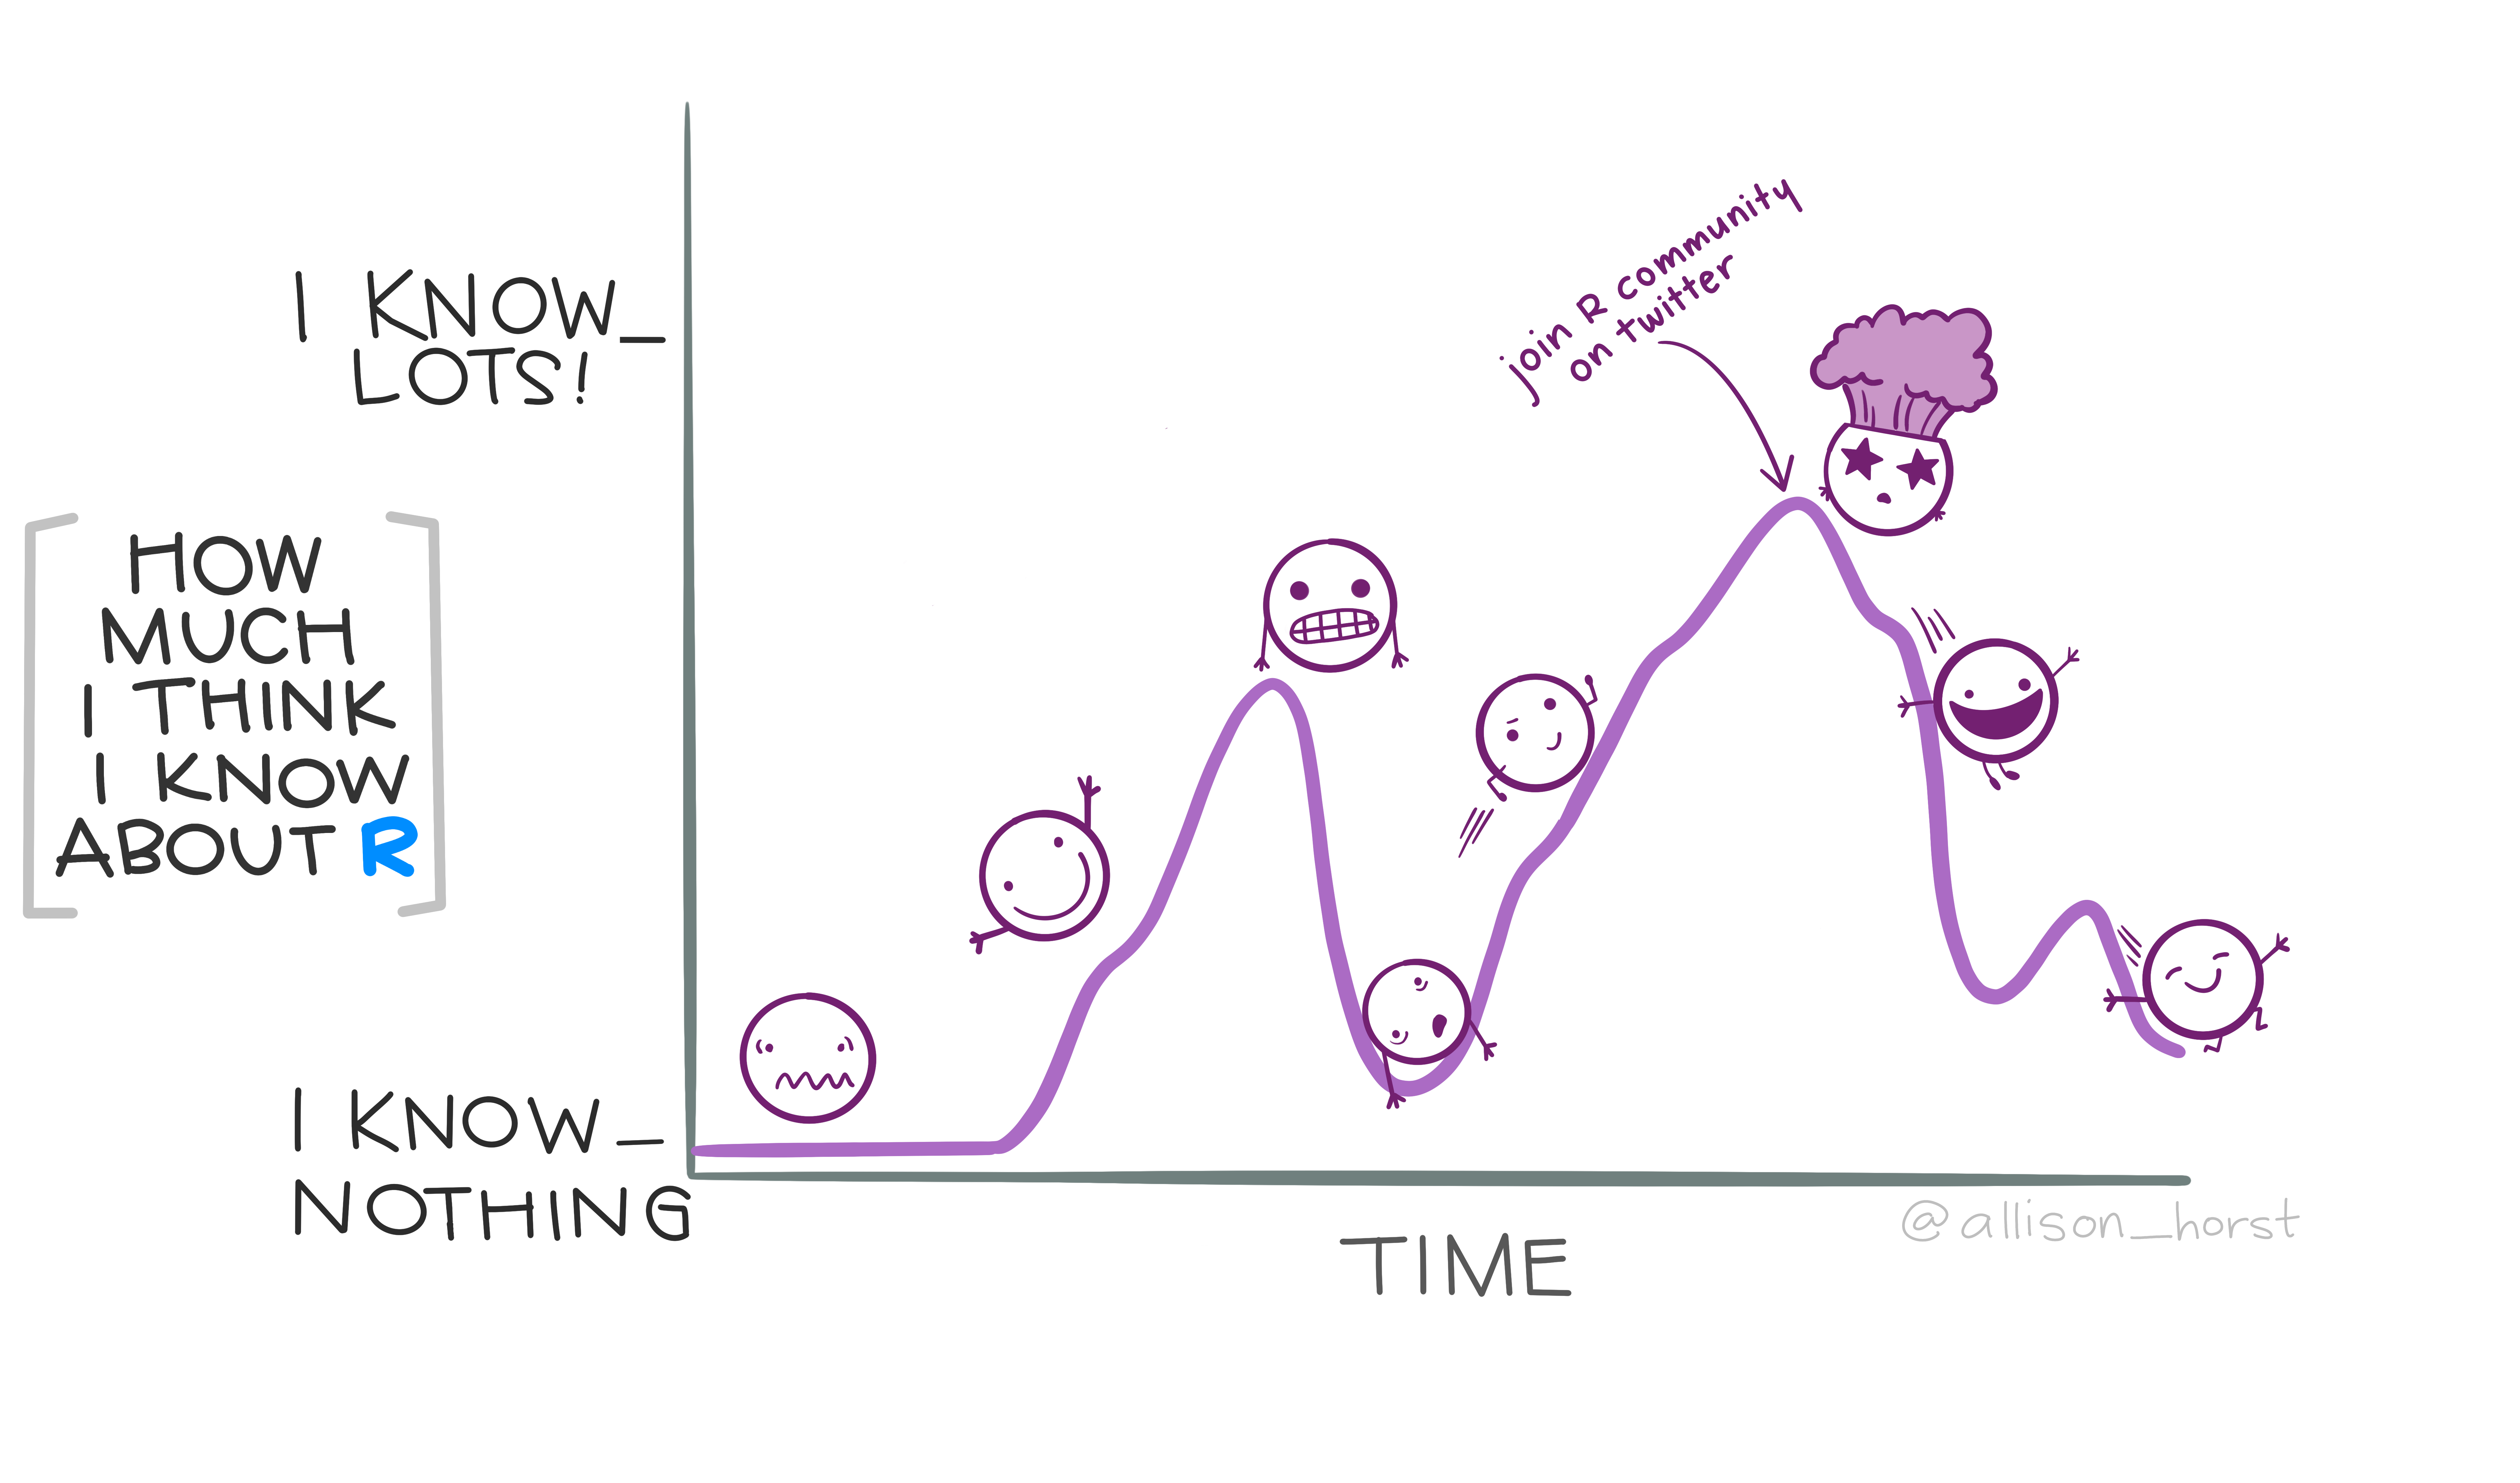
\includegraphics[width=0.8\textwidth,height=\textheight]{img/r_rollercoaster.png}

}

\caption{\label{fig-roller}Life is a roller-coaster. You just have to
ride it. Image credit: Allison Horst;
\url{https://github.com/allisonhorst/stats-illustrations}, CC-BY}

\end{figure}%

\subsubsection{Ab diesem Kapitel benötigen Sie
R}\label{ab-diesem-kapitel-benuxf6tigen-sie-r}

Bitte stellen Sie sicher, dass Sie R rechtzeitig einsatzbereit haben.
Weiter unten in diesem Kapitel finden Sie Installationshinweise
(Section~\ref{sec-install-r}). Falls Sie dieses Kapitel zum ersten Mal
bzw. sich noch nicht mir R auskennen, werden Sie vielleicht einigen
Inhalten begegnen, die Sie noch nicht gleich verstehen. Keine Sorge, das
ist normal. Mit etwas Übung wird Ihnen bald alles schnell von der Hand
ghen.

\subsubsection{Begleitvideos}\label{begleitvideos}

Schauen Sie sich malden YouTube-Kanal
\texttt{@sebastiansauerstatistics}\footnote{\url{https://www.youtube.com/@sebastiansauerstatistics}}
an und dort die Playlist ``R''\footnote{\url{https://www.youtube.com/playlist?list=PLRR4REmBgpIEaIyeNBgNGPgmhQJ_T1y8_}}.
Dort finden Sie einige Videos zum Thema R.

\subsection{Errrstkontakt}\label{errrstkontakt}

\subsubsection{Warum R?}\label{warum-r}

Gründe, die für den Einsatz von R sprechen:

\begin{enumerate}
\def\labelenumi{\arabic{enumi}.}
\item
  🆓 R ist kostenlos, andere Softwarepakete für Datenanalyse sind teuer.
  💸
\item
  📖 R und R-Befehle sind quelloffen, d.h. man kann sich die
  zugrundeliegenden Computerbefehle anschauen. Jeder kann prüfen, ob R
  vernünftig arbeitet. Alle können beitragen.
\item
  🆕 R hat die neuesten Methoden.
\item
  🫂 R hat eine große Community.
\item
  🪡 R ist maßgeschneidert für Datenanalyse.
\end{enumerate}

Allerdings gibt es auch abweichende Meinungen, s.
Figure~\ref{fig-bill-excel}.

\begin{figure}

\centering{


\includegraphics[width=0.5\textwidth,height=\textheight]{img/bill-gates-excel.jpg}

}

\caption{\label{fig-bill-excel}Manche finden Excel cooler als R, nicht
wahr, Bill Gates?}

\end{figure}%

\subsubsection{R und Reproduzierbarkeit}\label{r-und-reproduzierbarkeit}

\begin{definition}[Reproduzierbarkeit]\protect\hypertarget{def-repro}{}\label{def-repro}

Ein (wissenschaftlicher) Befunde ist reproduzierbar, wenn andere
Analystis mit dem gleichen experimentellen Setup zum gleichen Ergebnis
(wie in der ursprünglichen Analyse) kommen
{[}@plesser\_reproducibility\_2018{]}. \(\square\)

\end{definition}

Definition~\ref{def-repro} ist, etwas überspitzt, in
\textbf{?@fig-repro} wiedergegeben.


\includegraphics[width=0.5\textwidth,height=\textheight]{img/repro-star-struck.png}

Daten + Syntax + genaue Beschreibung der Messungen = reproduzierbar

:::::

\begin{example}[Aus der Forschung: Reproduzierbarkeit in der
Psychologie]\protect\hypertarget{exm-repro}{}\label{exm-repro}

~

\begin{quote}
Wie ist es um unsere Wissenschaft, Psychologie, bestellt? Haben die
Befunde Hand und Fuß?
\end{quote}

@obels\_analysis\_2020 haben die Reproduzierbarkeit in psychologischen
Studien untersucht. Sie berichten folgendes Ergebnis

\begin{quote}
We examined data and code sharing for Registered Reports published in
the psychological literature from 2014 to 2018 and attempted to
independently computationally reproduce the main results in each
article. Of the 62 articles that met our inclusion criteria, 41 had data
available, and 37 had analysis scripts available. Both data and code for
36 of the articles were shared. We could run the scripts for 31
analyses, and we reproduced the main results for 21 articles.
\(\square\)
\end{quote}

\end{example}

\subsubsection{R \& RStudio}\label{r-rstudio}

Wenn wir sagen, ``wir arbeiten mit R'', dann heißt das in unserem Fall
``wir arbeiten mit R und mit RStudio''.

\begin{figure}

\begin{minipage}{0.25\linewidth}

\includegraphics{img/R-logo.png}\end{minipage}%
%
\begin{minipage}{0.25\linewidth}

\text{\huge{\emoji{sparkling-heart}}}

\end{minipage}%
%
\begin{minipage}{0.50\linewidth}

\includegraphics{img/rlogo.png}\end{minipage}%

\end{figure}%

@ismay\_statistical\_2020 zeigen eine schöne Analogie, was der
Unterschied von \emph{R} und \emph{RStudio} ist, s.
Figure~\ref{fig-r-rstudio}.\footnote{Streng genommen ist RStudio für die
  Datenanalyse irrelevant, aber RStudio ist praktisch, Sie werden es
  nicht missen wollen.}

\begin{figure}

\centering{

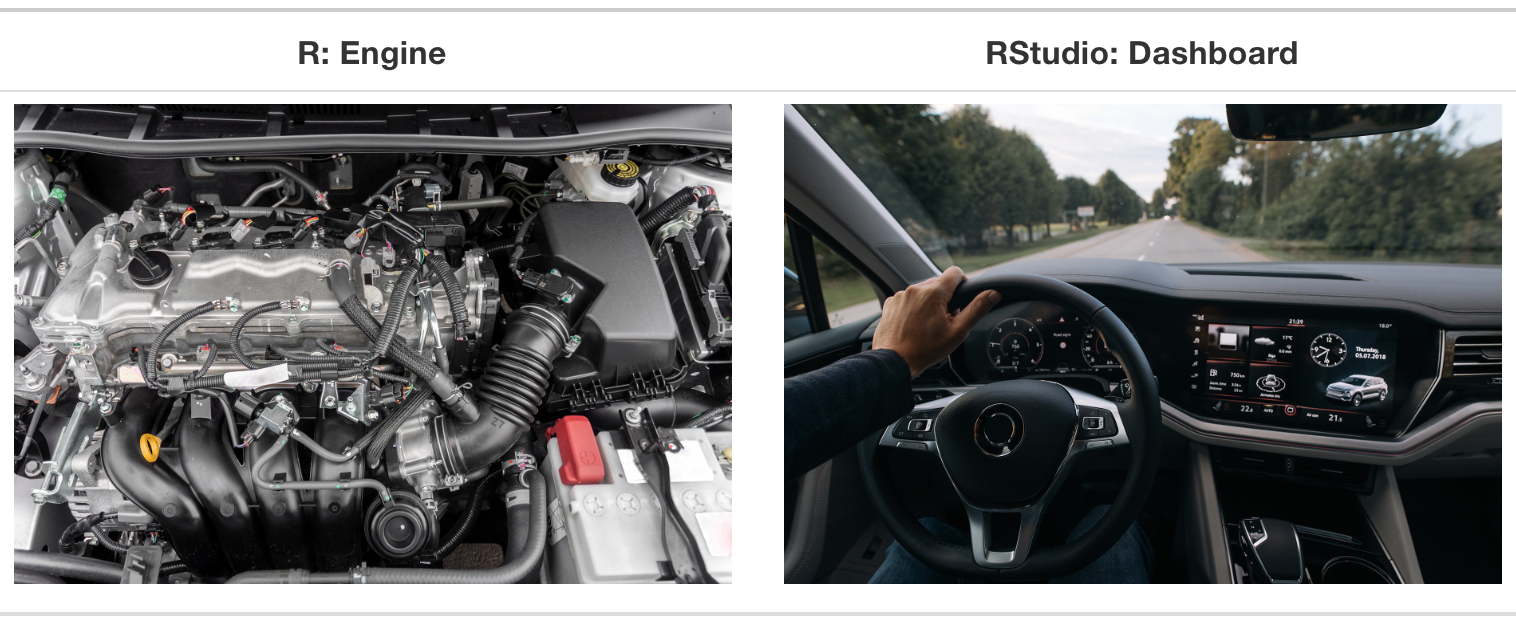
\includegraphics[width=5.05in,height=\textheight]{img/r_vs_rstudio_1.png}

}

\caption{\label{fig-r-rstudio}R vs.~RStudio: R macht die Arbeit, RStudio
ist für Komfort und Übersicht}

\end{figure}%

Kurz gesagt: Das eigentlich Arbeiten besorgt R. Für den Komfort und die
Schönheit ist RStudio zuständig. Auch eine Art von Arbeitsteilung!

Hier sehen Sie einen Screenshot von der Oberfläche von RStudio, s.
Figure~\ref{fig-rstudio}.

\begin{figure}

\centering{

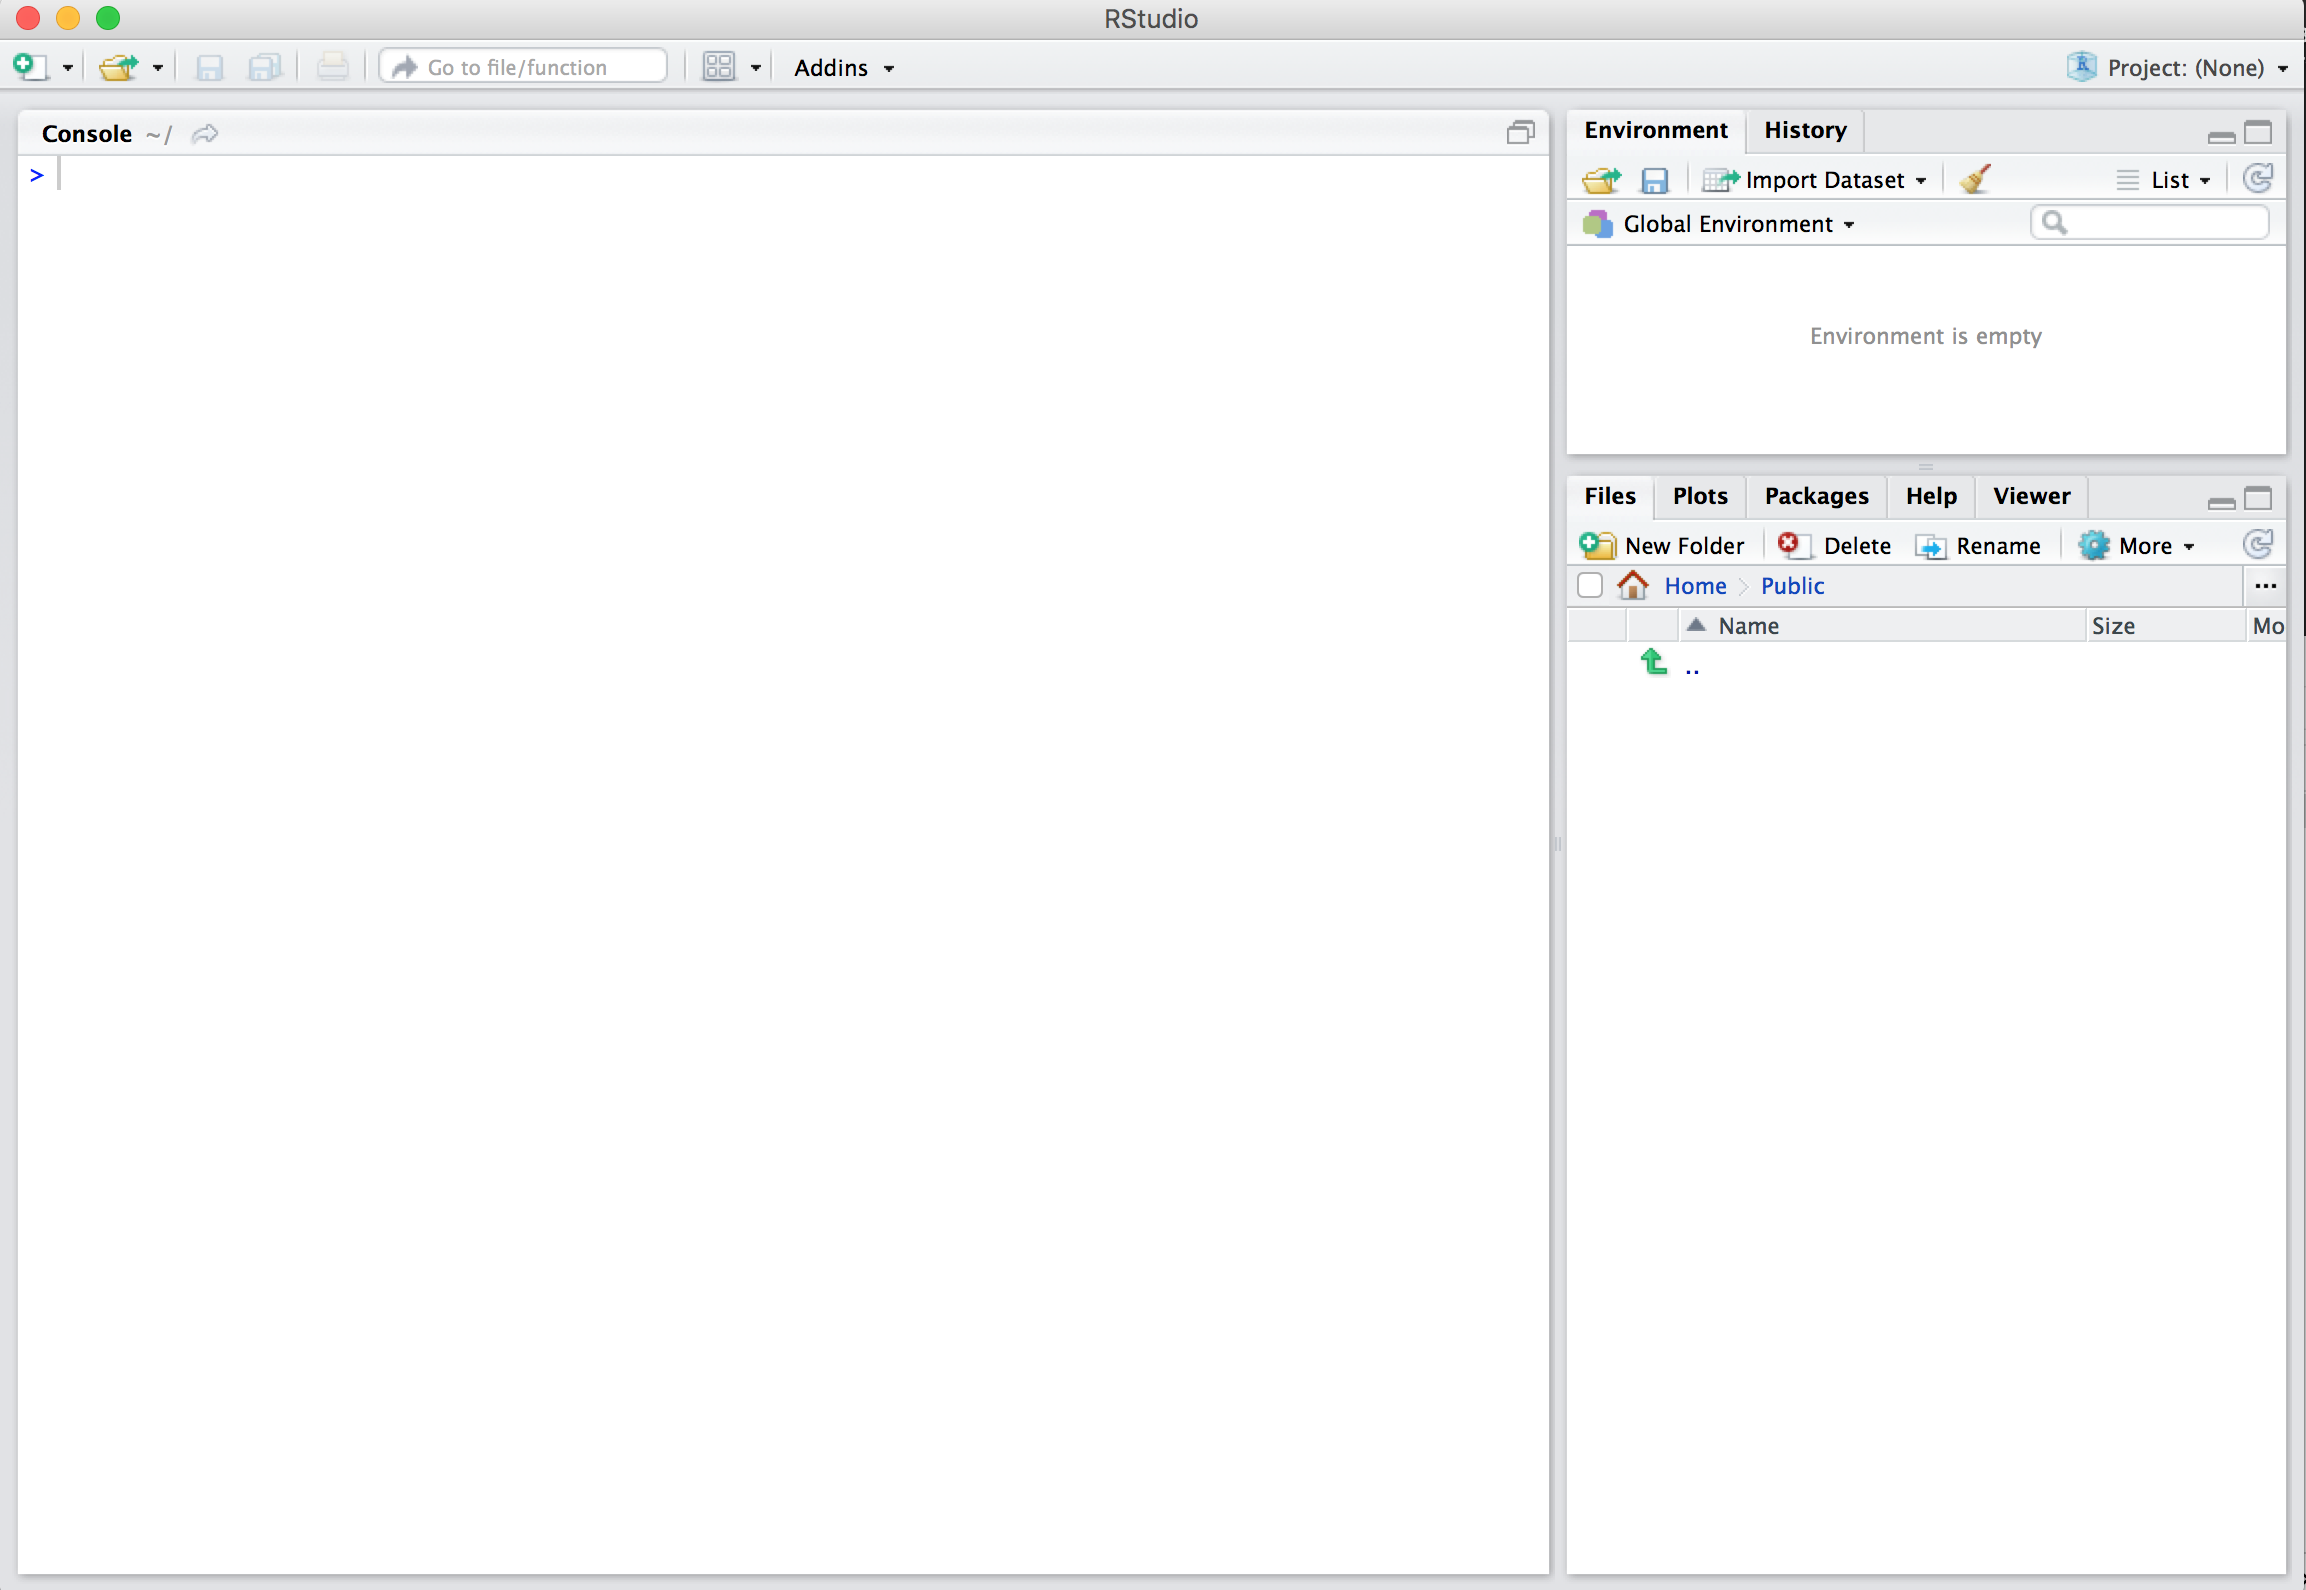
\includegraphics{img/rstudio.png}

}

\caption{\label{fig-rstudio}So sieht RStudio aus}

\end{figure}%

\subsection{Installation von R und RStudio}\label{sec-install-r}

\subsubsection{Installation von R}\label{installation-von-r}

R ist ein Softwarepaket für statistische Berechnungen\footnote{Mehr
  Infos finden sich hier:
  \url{https://de.wikipedia.org/wiki/R_\%28Programmiersprache\%29}}.
Laden Sie es für Ihr Betriebssytem herunter:

\begin{itemize}
\tightlist
\item
  \href{https://cloud.r-project.org/bin/windows/base/}{Windows}
\item
  \href{https://cloud.r-project.org/bin/macosx/}{MacOS}
\item
  \href{https://cloud.r-project.org/bin/linux/}{Linux}
\end{itemize}

Mehr Infos zu R finden Sie unter
\url{https://cloud.r-project.org/}.\footnote{Wenn Sie gefragt werden,
  dass Sie einen ``Mirror'' auswählen sollen, heißt das, Sie sollen
  einen Computer (Server) wählen, von dem Sie R herunterladen. Der
  sollte möglichst nicht zu weit weg stehen, dann spart es vielleicht
  etwas Zeit und Bandbreite.}

Wenn Sie die Installationsdatei heruntergeladen haben, öffnen Sie diese
Datei (Doppelklick) und Sie werden durch die Installation
geführt.\footnote{Sie benötigen Admin-Rechte auf Ihrem Computer.}

\subsubsection{Installation von RStudio
Desktop}\label{installation-von-rstudio-desktop}

RStudio ist eine \emph{graphische Benutzeroberfläche} (graphical user
interface, GUI) für R, plus ein paar Goodies\footnote{in Form einer
  \emph{intergrierten Entwicklungsumgebung} (integrated development
  environment, IDE:
  \url{https://en.wikipedia.org/wiki/Integrated_development_environment}))}.

Laden Sie zunächst die \emph{Desktop-Version} von RStudio herunter für
Ihr Betriebssystem (Windows, MacOS, Linux) vom Anbieter (Posit)
herunter. \footnote{\url{https://posit.co/download/rstudio-desktop/}}.

Wenn Sie die Installationsdatei heruntergeladen haben, öffnen Sie diese
Datei (Doppelklick) und Sie werden durch die Installation
geführt.\footnote{Sie benötigen u.U. Admin-Rechte auf Ihrem Computer.}

\subsubsection{RStudio Cloud}\label{rstudio-cloud}

\paragraph{RStudio Cloud als Alternative zu
RStudio}\label{rstudio-cloud-als-alternative-zu-rstudio}

RStudio Cloud\footnote{\url{https://rstudio.cloud/}; neuerdings auch
  ``Posit Cloud'' genannt} ist ein Webdienst von Posit/RStudio (zum Teil
kostenlos), also \emph{RStudio online}: Man kann damit online mit R
arbeiten. Die Oberfläche ist praktisch identisch zur Desktop-Version, s.
Figure~\ref{fig-rstudio-cloud}. Sie können es als Alternative zur
Installation von RStudio auf Ihrem Computer verwenden. Ein Vorteil von
RStudio Cloud ist, dass man als Nutzer \emph{nichts installieren} muss
und dass es \emph{auch auf Tablets} läuft (im Gegensatz zur
Desktop-Version von RStudio). Ein Nachteil ist, dass es etwas langsamer
ist und nur für ein gewisses Zeitvolumen kostenlos. Sie müssen sich ein
Konto anlegen, um den Dienst nutzen zu können.

\begin{figure}

\centering{

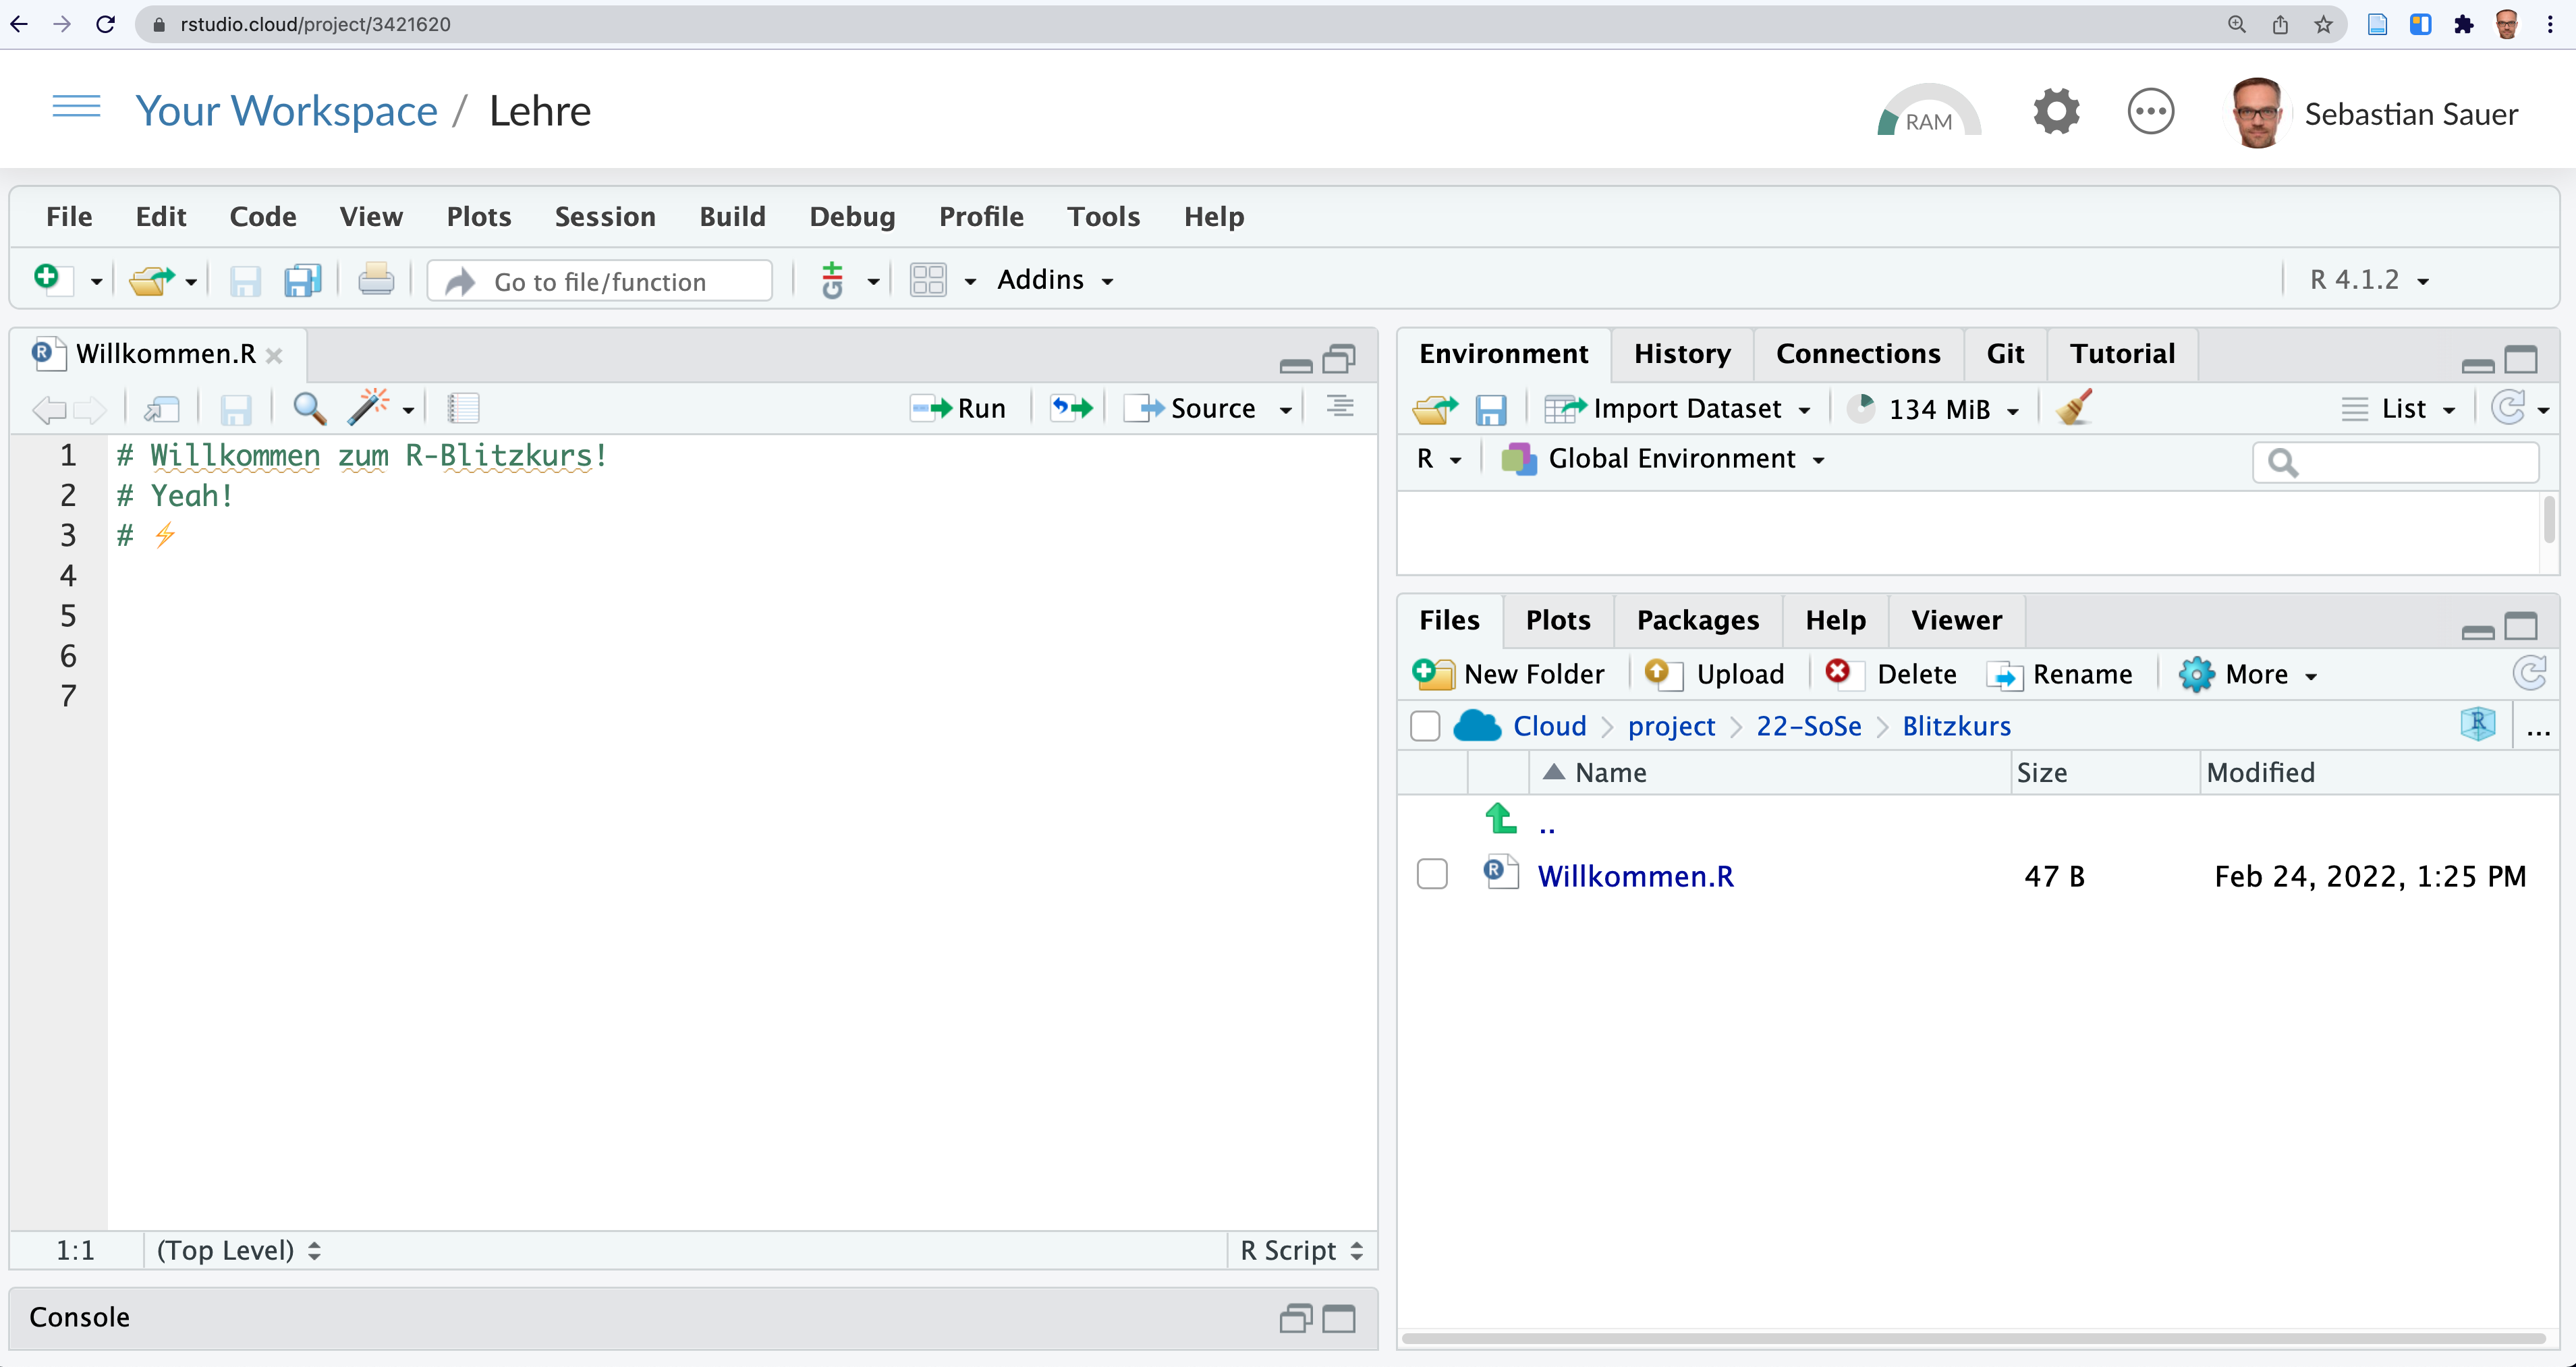
\includegraphics{img/rstudio-cloud.png}

}

\caption{\label{fig-rstudio-cloud}So sieht RStudio Cloud aus. Genau wie
RStudio Desktop}

\end{figure}%

\paragraph{Vertiefung}\label{vertiefung}

Wenn Ihr Dozent Ihnen einen Projektordner bzw. einen Link dazu
bereitstellt, ist das komfortabel, da der Dozent dann schon Pakete
installieren, Daten bereitstellen und andere Nettigkeit vorbereiten kann
für Sie. Allerdings müssen Sie den Projektordner in Ihrem Konto
abspeichern, wenn Sie etwas speichern möchten, da Sie vermutlich keine
Schreibrechte im Projektordner Ihres Dozenten haben. Klicken Sie dazu
auf ``Save a permanent copy'', s. Figure~\ref{fig-perm-copy}.

\begin{figure}

\centering{


\includegraphics{img/rstudio-save-a-permanent-copy.png}

}

\caption{\label{fig-perm-copy}Einen Projektordner im eigenen Konto
abspeichern, um Schreibrechte zu haben}

\end{figure}%

Sie können auch von der Cloud exportieren, also Ihre Syntaxdatei
herunterladen. Klicken Sie dazu im Reiter ``Files'' auf
\texttt{More\ \textgreater{}\ Export\ ...}.

\subsection{RStudio starten, nicht R}\label{rstudio-starten-nicht-r}

Wir verwenden beide Programme (R und RStudio). Aber wir \emph{öffnen
nur} RStudio. RStudio findet selbständig R und öffnet dieses
``heimlich''. Öffnen Sie nicht noch extra R (sonst wäre R zweifach
geöffnet).

Anstelle von \emph{RStudio Desktop} (auf Ihrem Computer/Desktop) können
Sie auch die \emph{RStudio Cloud} (die Online-Version ) starten.

\subsection{R-Pakete}\label{r-pakete}

\subsubsection{Was sind R-Pakete?}\label{was-sind-r-pakete}

Typisch für R ist sein modularer Aufbau: Man kann eine große Zahl an
Erweiterungen (``Pakete'', engl. \emph{packages}) installieren, alle
kostenlos. In R Paketen ``wohnen'' R-Befehle, also Dinge, die R kann,
``Skills'' sozusagen. Außerdem können in R-Paketen auch Daten
bereitgestellt werden. Damit man die Inhalte eines R-Pakets nutzen kann,
muss man es zuerst installieren und dann starten.

Man kann sich daher ein R-Paket vorstellen wie ein Buch: Wenn R es
gelesen hat, dann kennt es die Inhalte. Diese Inhalte könnten
irgendwelche Formeln, also Berechnungen sein. Es könnte aber die
``Bauanleitung'' für ein schönes Diagramm sein.

Ist ein spezielles R-Paket auf Ihrem Computer installiert, so können Sie
diese Funktionalität nutzen.

Die Zahl an diesen ``Paketen'' ist groß; zur Verdeutlichung s.
Figure~\ref{fig-pakete}.

\begin{figure}

\centering{

\subsubsection{Viele Pakete}

\centering{

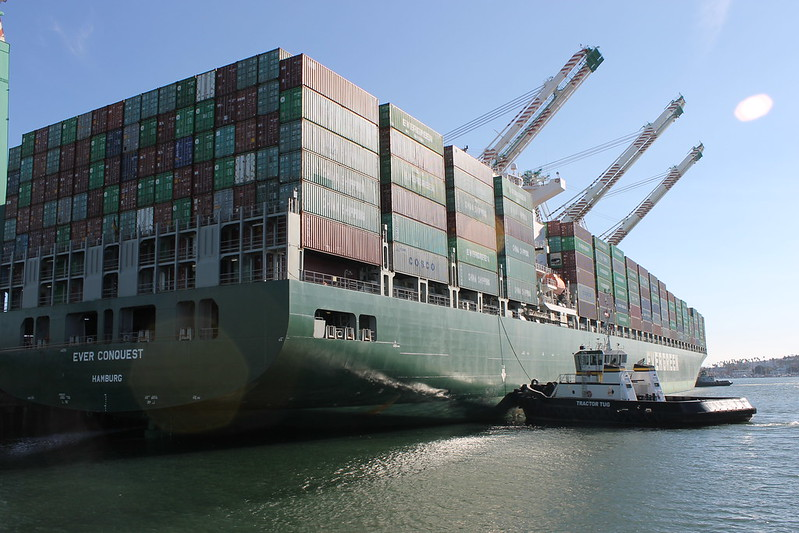
\includegraphics[width=0.5\textwidth,height=\textheight]{img/11102039694_d42ca1ff1c_c.jpg}

}

\subcaption{\label{fig-ship}Containershiff mit vielen Paketen, Corey
Seeman, CC-BY-NC 20, Flickr.com}

\subsubsection{Es kommen viele dazu}

\centering{

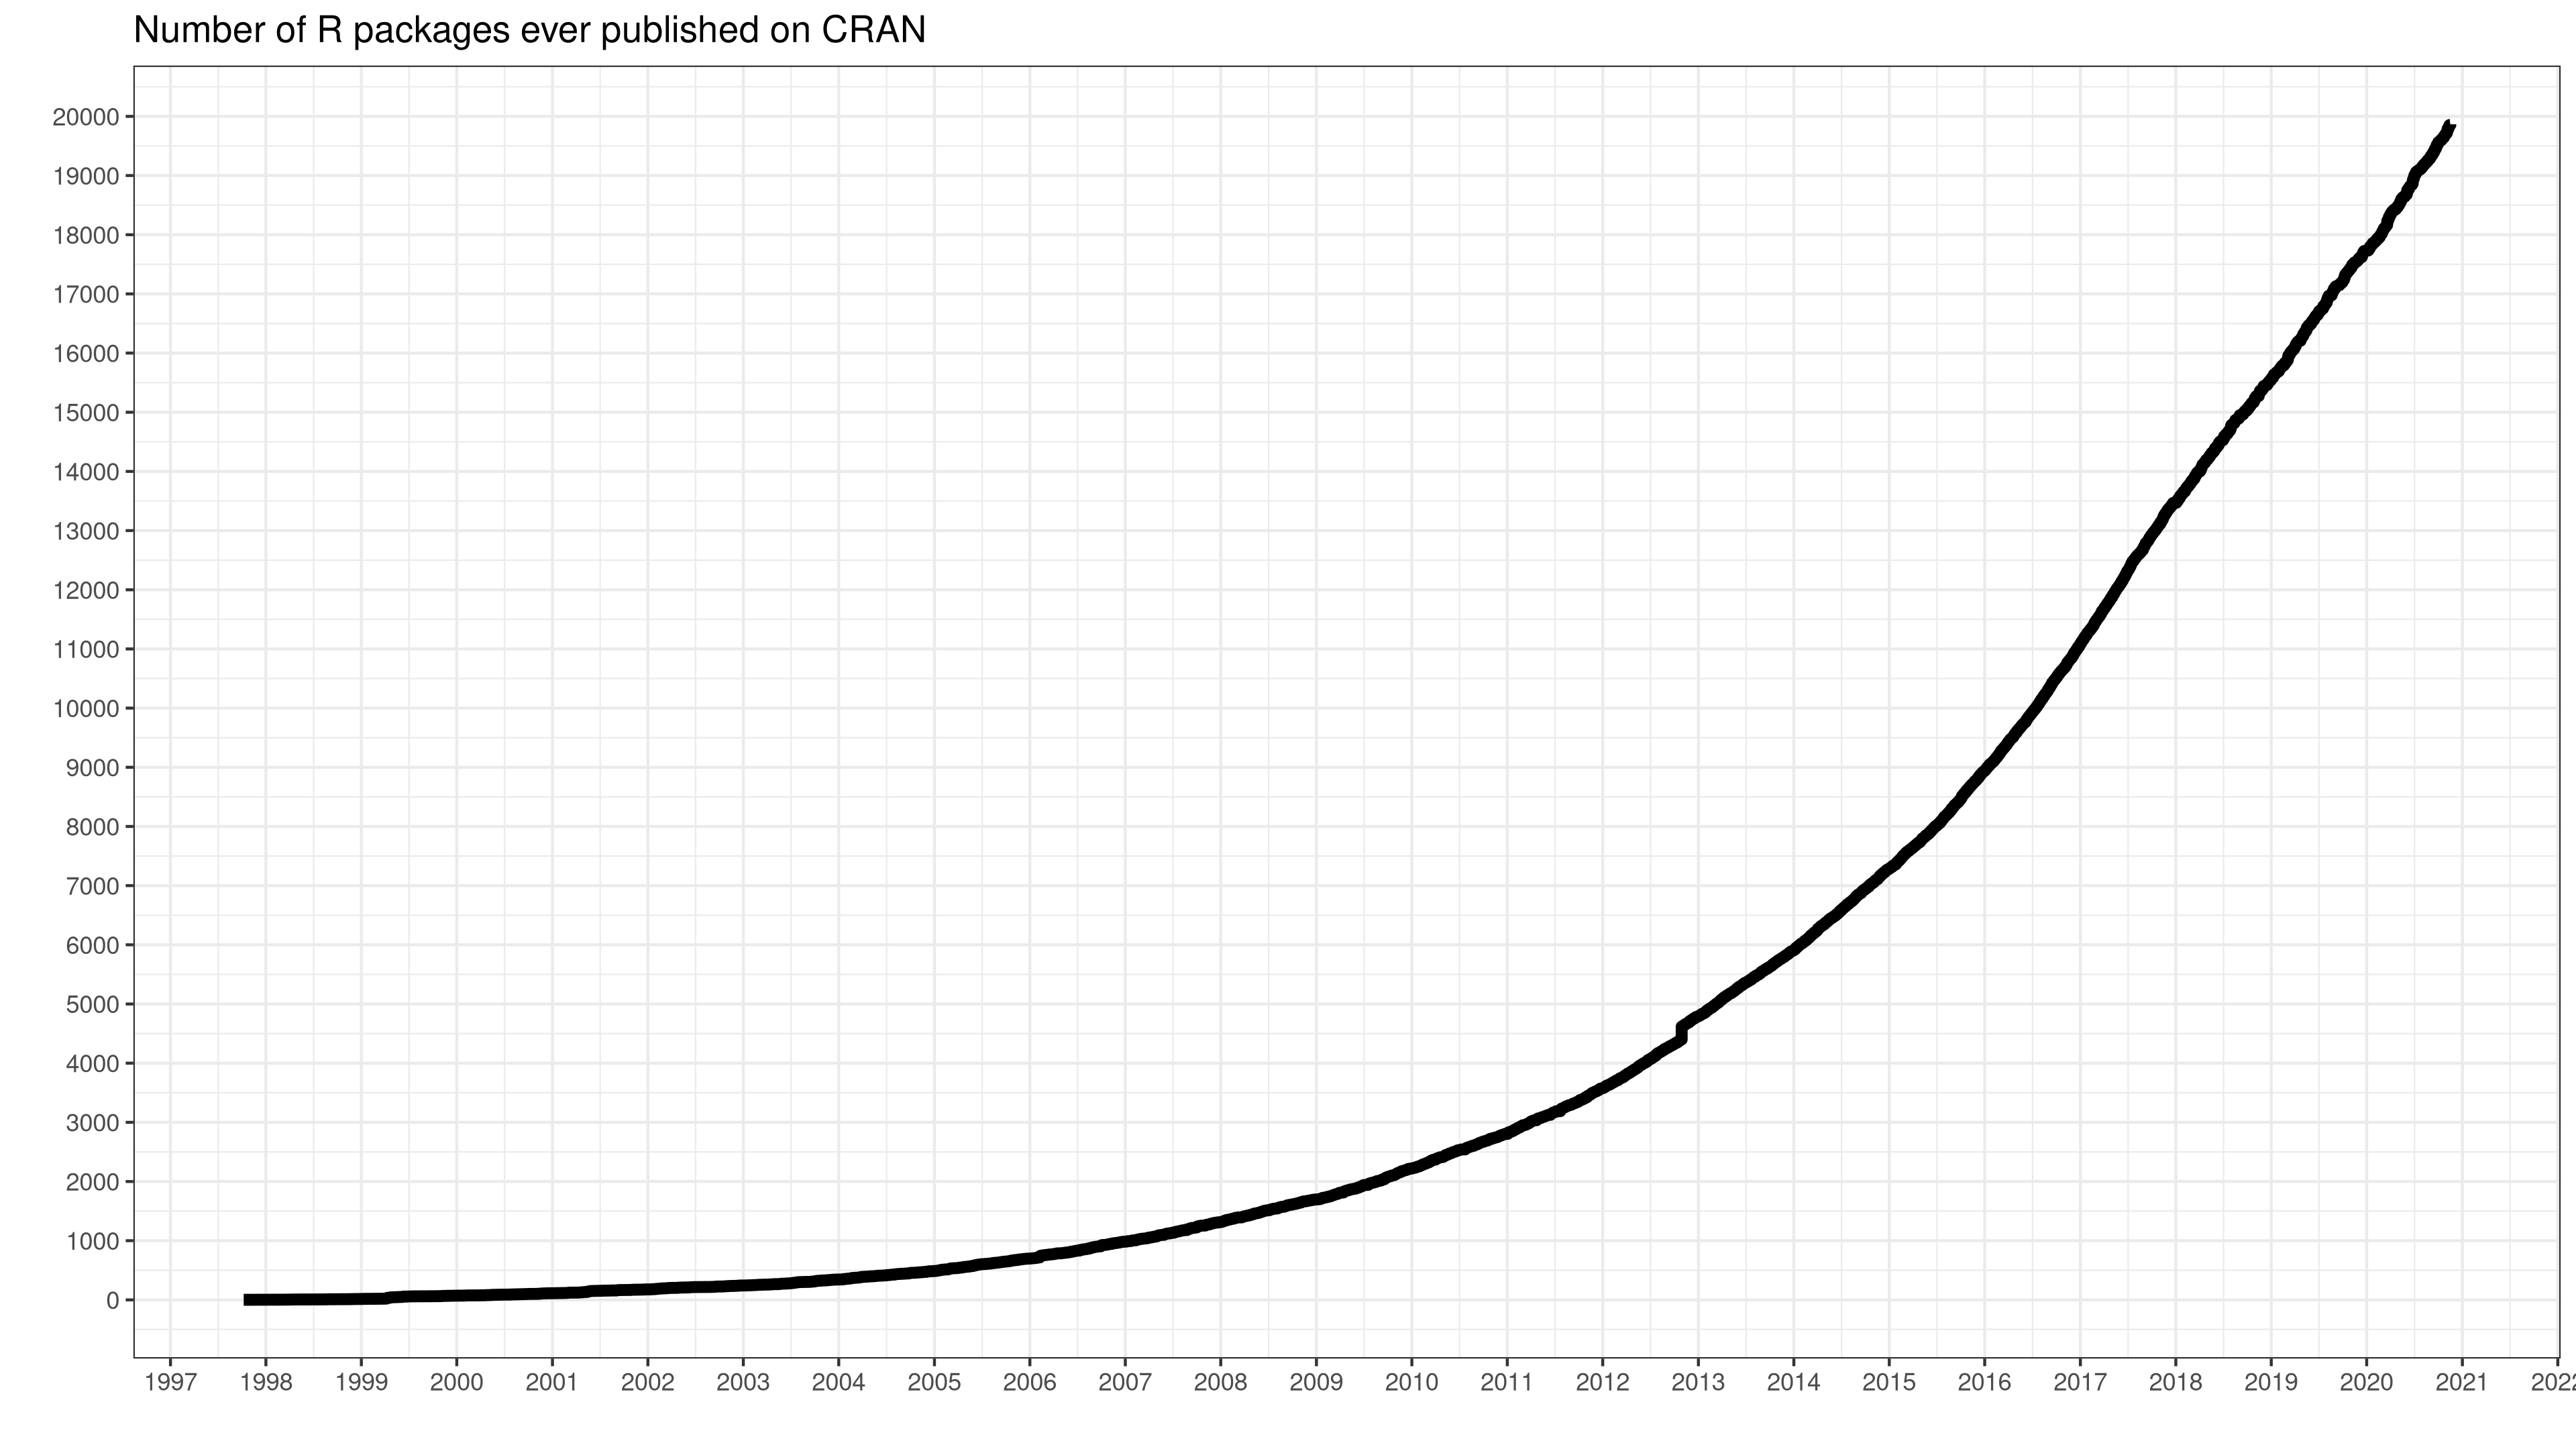
\includegraphics{img/number-of-submitted-packages-to-CRAN.png}

}

\subcaption{\label{fig-cran}Die Anzahl der R-Pakete ist exponenziell
gewachsen}

Es gibt viele R-Pakete.

}

\caption{\label{fig-pakete}}

\end{figure}%

\emph{Erweiterungen} kennt man von vielen Programmen, sie werden auch
\emph{Add-Ons}, \emph{Plug-Ins} oder sonstwie genannt. Man siehe zur
Verdeutlichung Erweiterungen beim Broswer Chrome,
Figure~\ref{fig-chrome}.

\begin{figure}

\centering{

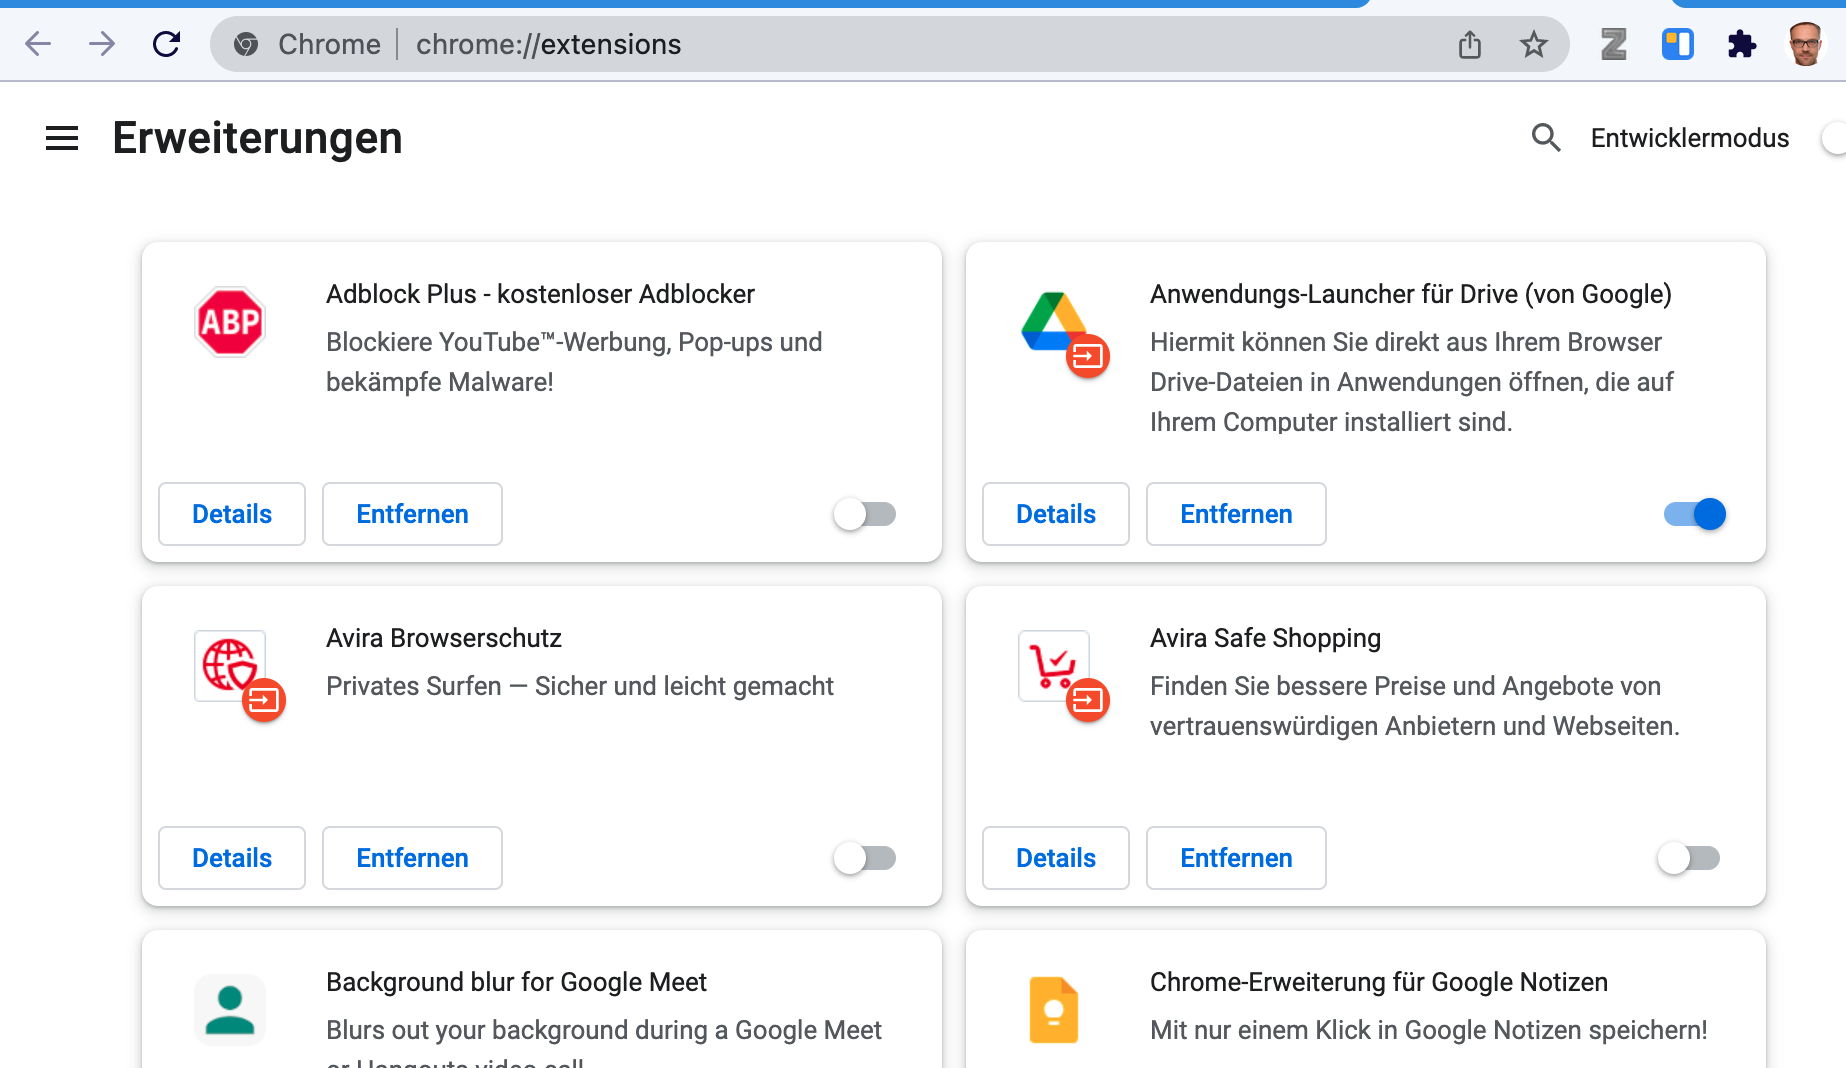
\includegraphics[width=0.5\textwidth,height=\textheight]{img/chrome-extensions.png}

}

\caption{\label{fig-chrome}Erweiterungen beim Browser Chrome}

\end{figure}%

Die Anzahl der R-Pakete ist groß; allein auf dem ``offiziellen
Web-Store'' (nennt sich ``CRAN'') von R gibt es ca. 20,000 Pakete (vgl.
Figure~\ref{fig-cran});
\href{https://gist.github.com/daroczig/3cf06d6db4be2bbe3368}{Stand:
2022; Quelle}). Und es kommen immer mehr dazu.

\subsubsection{Pakete installieren}\label{install-r-pckgs}

Wie jede Software muss man Pakete (Erweiterungen für R) erst einmal
installieren, bevor man sie verwenden kann. Ja, einmal installieren
reicht.

Das geht komfortabel, wenn man beim Reiter \emph{Packages} auf
\emph{Install} klickt (s. Figure~\ref{fig-pckgs}) und dann den Namen des
zu installierenden Pakets eingibt.

\begin{figure}

\begin{minipage}{0.50\linewidth}

\centering{

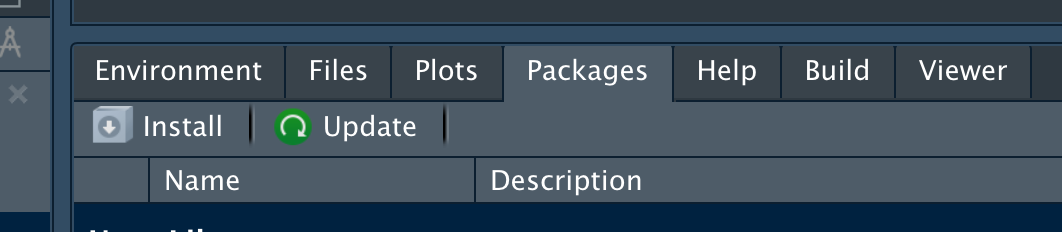
\includegraphics{img/install-packages.png}

}

\subcaption{\label{fig-install-packages}Klicken Sie auf ``Install'' im
Reiter ``Packages'', um R-Pakete zu installieren}

\end{minipage}%
%
\begin{minipage}{0.50\linewidth}

\centering{

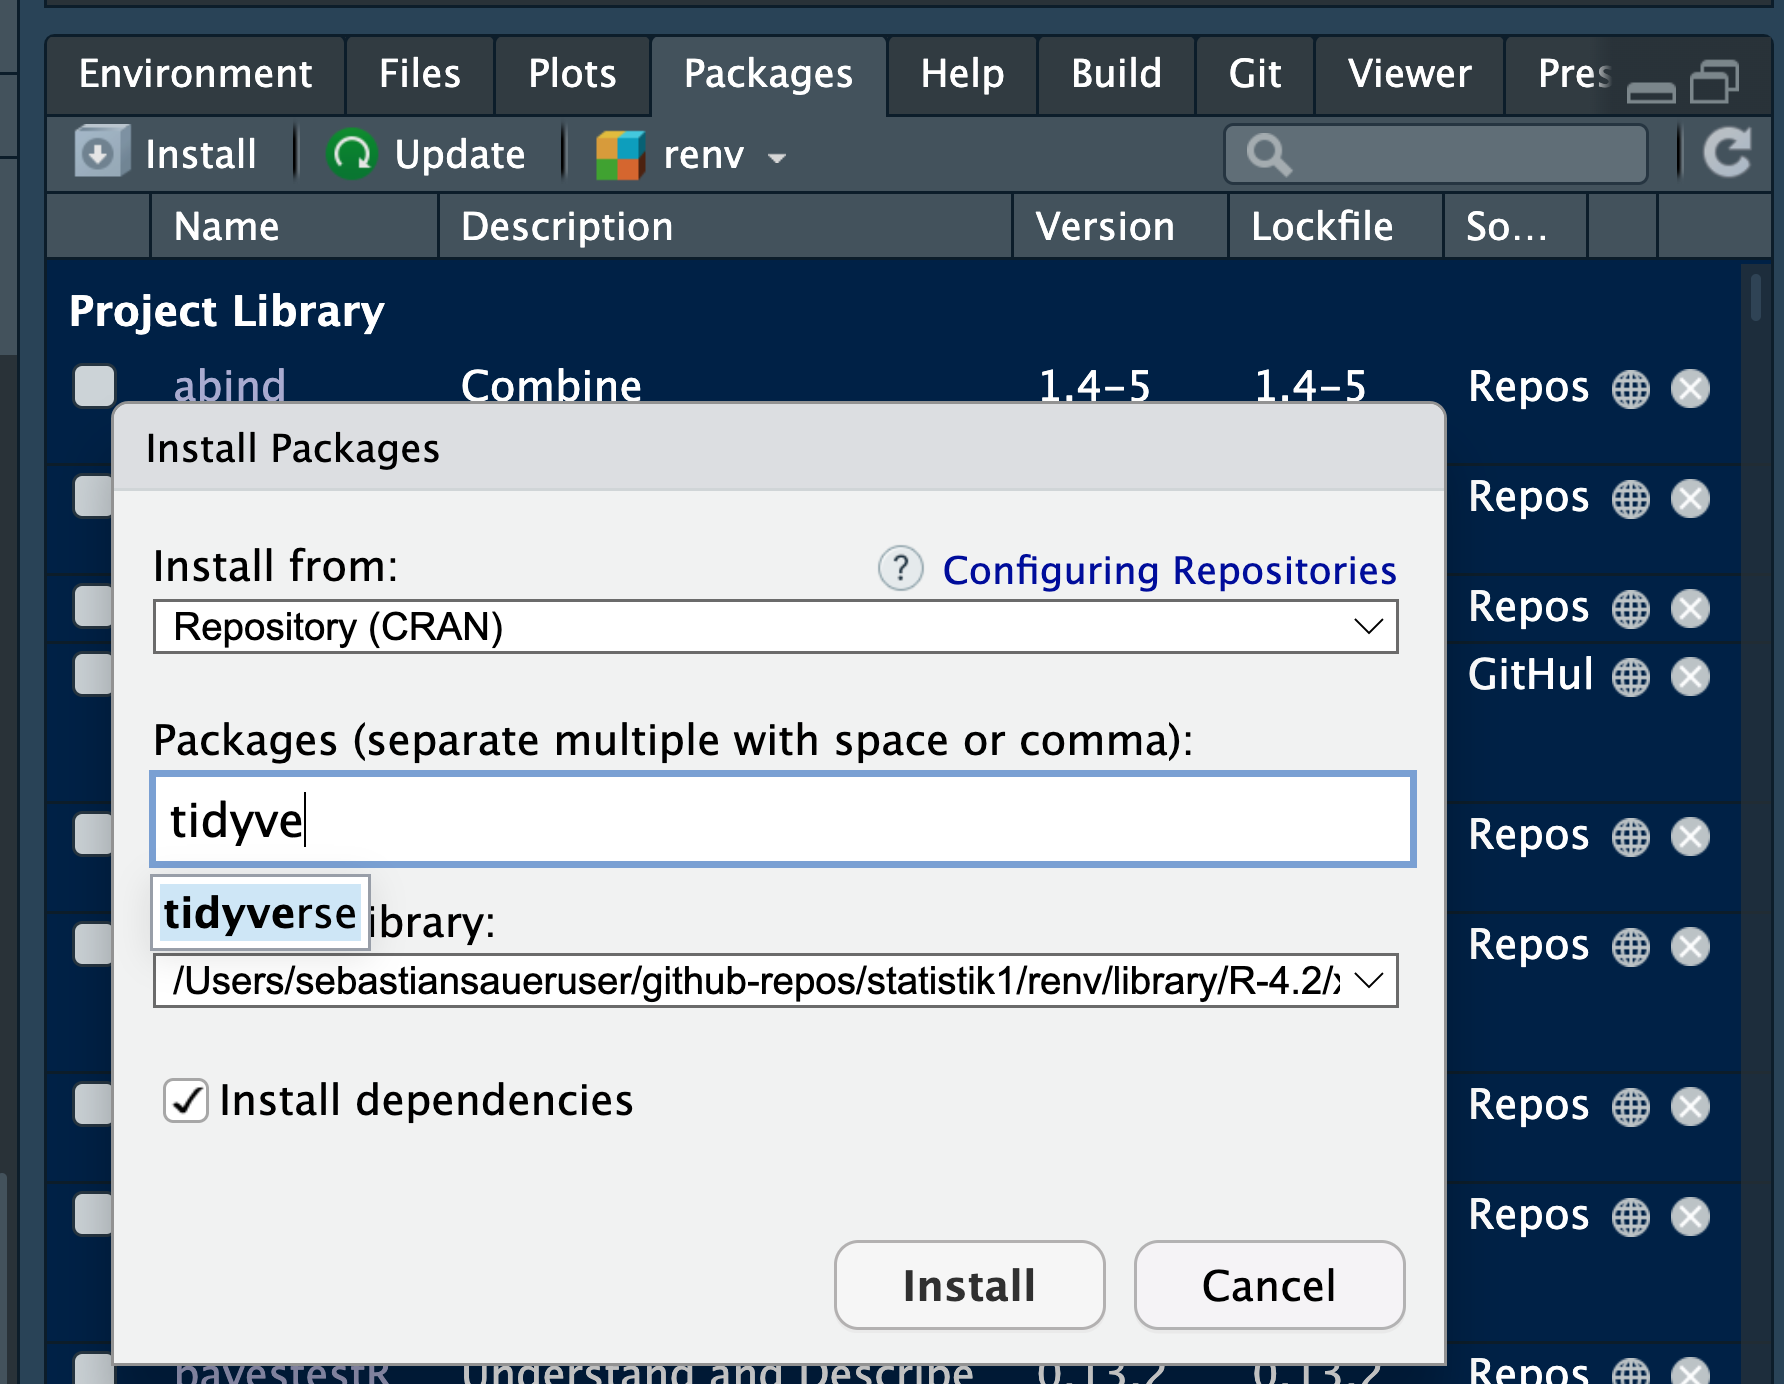
\includegraphics{img/install-packages3.png}

}

\subcaption{\label{fig-so-installieren}Geben Sie den Namen des zu
installierenden R-Pakets in dieser Maske ein}

\end{minipage}%

\caption{\label{fig-pckgs}So installiert man Pakete in R.}

\end{figure}%

\begin{quote}
Welche R-Pakete sind denn schon installiert?
\end{quote}

Im Reiter \emph{Packages} können Sie nachschauen, welche Pakete auf
Ihrem Computer schon installiert sind. Diese Pakete brauchen Sie
logischerweise dann \emph{nicht} noch mal installieren, s.
Figure~\ref{fig-paket-installiert}.

\begin{figure}

\centering{

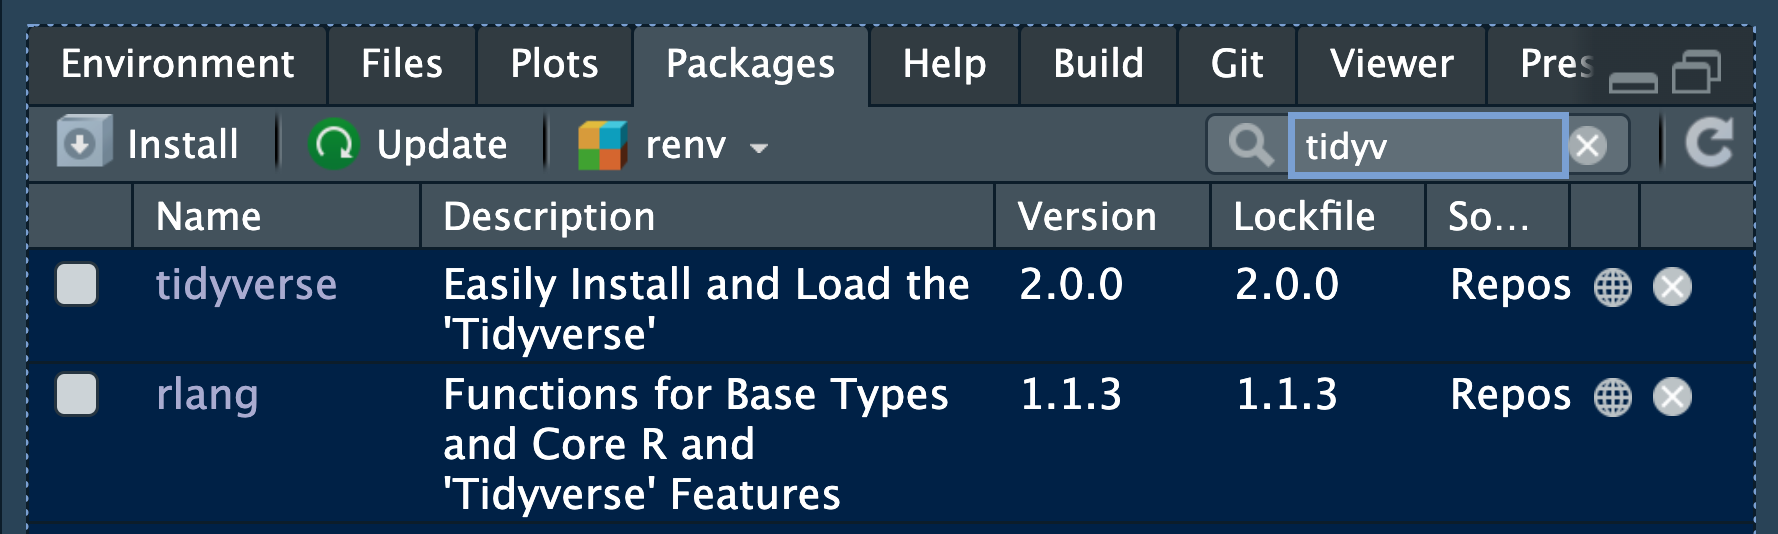
\includegraphics{img/paket-installiert.png}

}

\caption{\label{fig-paket-installiert}So sehen Sie, ob ein R-Paket auf
Ihrem System installiert ist}

\end{figure}%

Alternativ können Sie zum Installieren von Paketen auch den Befehl
\texttt{install.packages()} verwenden. Also zum Beispiel
\texttt{install.packages(tidyverse)} um das Paket \texttt{tidyverse} zu
installieren.

\begin{quote}
Ja, aber welche R-Pakete ``soll'' ich denn installieren, welche brauch
ich denn?
\end{quote}

Im Moment sollten Sie die folgenden Pakete installiert haben:

\begin{itemize}
\tightlist
\item
  \texttt{tidyverse}
\item
  \texttt{easystats}
\end{itemize}

Wenn Sie die noch nicht installiert haben sollten, dann können Sie das
jetzt ja nachholen.\footnote{Übrigens sind \texttt{tidyverse} und
  \texttt{easystats} Pakete, die nur dafür da sind, mehrere Pakete zu
  installieren. So gehören z.B. zu \texttt{tidyverse} die Pakete
  \texttt{ggplot} (Daten verbildlichen) und \texttt{dplyr} (Datenjudo).
  Damit wir nicht alle Pakete einzeln installieren und starten müssen,
  bietet uns das Paket \texttt{tidyverse} den Komfort, alle die Pakete
  dieser ``Sammlung'' auf einmal zu starten. Praktisch.}

\begin{tcolorbox}[enhanced jigsaw, coltitle=black, colframe=quarto-callout-caution-color-frame, opacityback=0, toprule=.15mm, opacitybacktitle=0.6, arc=.35mm, titlerule=0mm, toptitle=1mm, title=\textcolor{quarto-callout-caution-color}{\faFire}\hspace{0.5em}{Caution}, bottomtitle=1mm, leftrule=.75mm, breakable, rightrule=.15mm, colbacktitle=quarto-callout-caution-color!10!white, bottomrule=.15mm, colback=white, left=2mm]

Bevor Sie ein R-Paket (oder überhaupt irgendwelche Software)
installieren/updaten, sollten Sie das R-Paket schließen/beenden. Sonst
schrauben Sie an einem elektrischen Gerät herum, das noch unter Strom
steht (nicht gut). Die einfachste Art, alle Pakete zu beenden ist,
\texttt{Session\ \textgreater{}\ Restart\ R} zu klicken (in
RStudio).\(\square\)

\end{tcolorbox}

\subsubsection{Pakete starten}\label{pakete-starten}

Wenn Sie ein Softwareprogramm - nichts anderes sind R-Pakete -
installiert haben, müssen Sie es noch \emph{starten}.

Merke: Ein bestimmtes R-Paket muss man nur \emph{einmalig installieren}.
Aber man muss es \emph{jedes Mal neu starten}, wenn man R (bzw. RStudio)
startet.

Sie erkennen leicht, ob ein Paket gestartet ist, wenn Sie ein Häkchen
vor dem Namen des Pakets in der Paketliste (Reiter \emph{Packages})
sehen, s. Abbildung Figure~\ref{fig-install-packages}.\footnote{Dieses
  Video
  \url{https://www.youtube.com/watch?v=Yej9xzKQ3yI&list=PLRR4REmBgpIEaIyeNBgNGPgmhQJ_T1y8_&index=26}
  verdeutlicht den Unterschied zwischen \emph{Installation} und
  \emph{Starten} eines R-Pakets.}

\subsection{Mit R arbeiten}\label{mit-r-arbeiten}

\subsubsection{Projekte in R}\label{projekte-in-r}

Ein \emph{Projekt} in RStudio (s. Figure~\ref{fig-projects}) ist
letztlich ein Ordner, der als ``Basis'' für eine Reihe von Dateien
verwendet wird. Sagen wir, das Projekt heißt \texttt{cool\_stuff}.
RStudio legt uns diesen Ordner an einem von uns gewählten Platz auf
unserem Computer an. Das ist ganz praktisch, weil man dann sagen kann
``Hey R, nimmt die Datei `daten.csv'\,'', ohne einen Pfad anzugeben.
Vorausgesetzt, die Datei liegt auch im Projektordner
(\texttt{cool\_stuff}).

Projekte kann anlegen mit Klick auf das Icon, das einen Quader mit dem
Buchstaben R darin anzeigt (s. Figure~\ref{fig-rstudio-projekte}).
RStudio-Projekte machen Ihr Leben leichter (s.
Figure~\ref{fig-projects}).

\begin{figure}

\begin{minipage}{0.50\linewidth}

\centering{

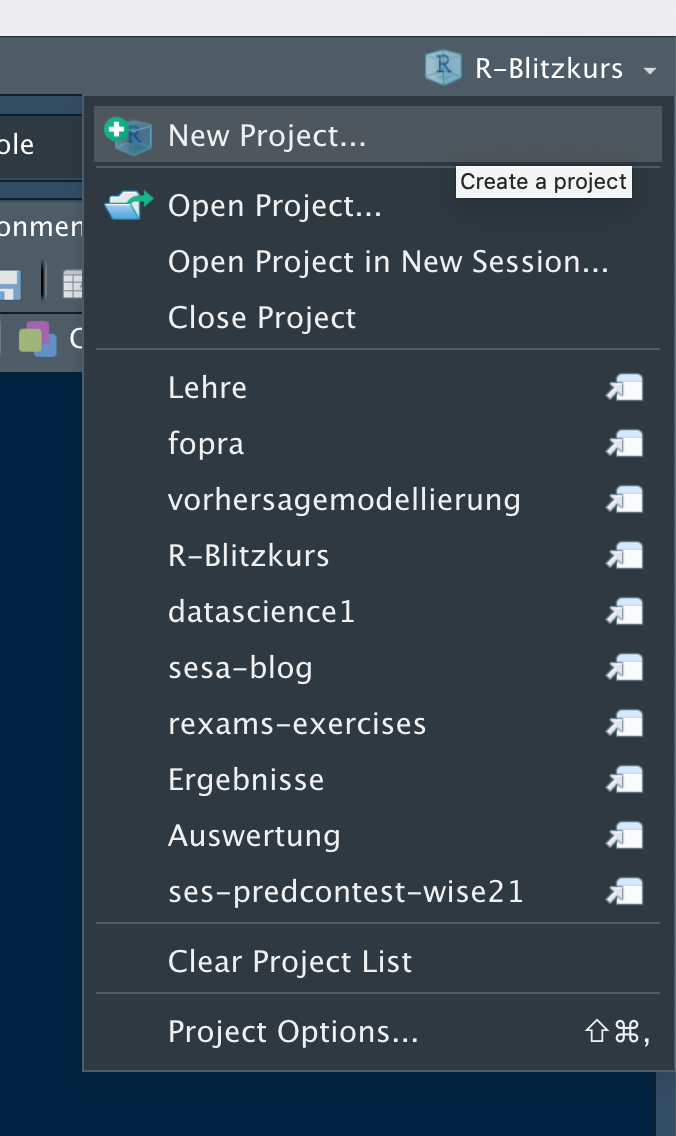
\includegraphics[width=0.5\textwidth,height=\textheight]{img/rstudio-projekte.png}

}

\subcaption{\label{fig-rstudio-projekte}RStudio-Projekte, Beispiele}

\end{minipage}%
%
\begin{minipage}{0.50\linewidth}

\centering{

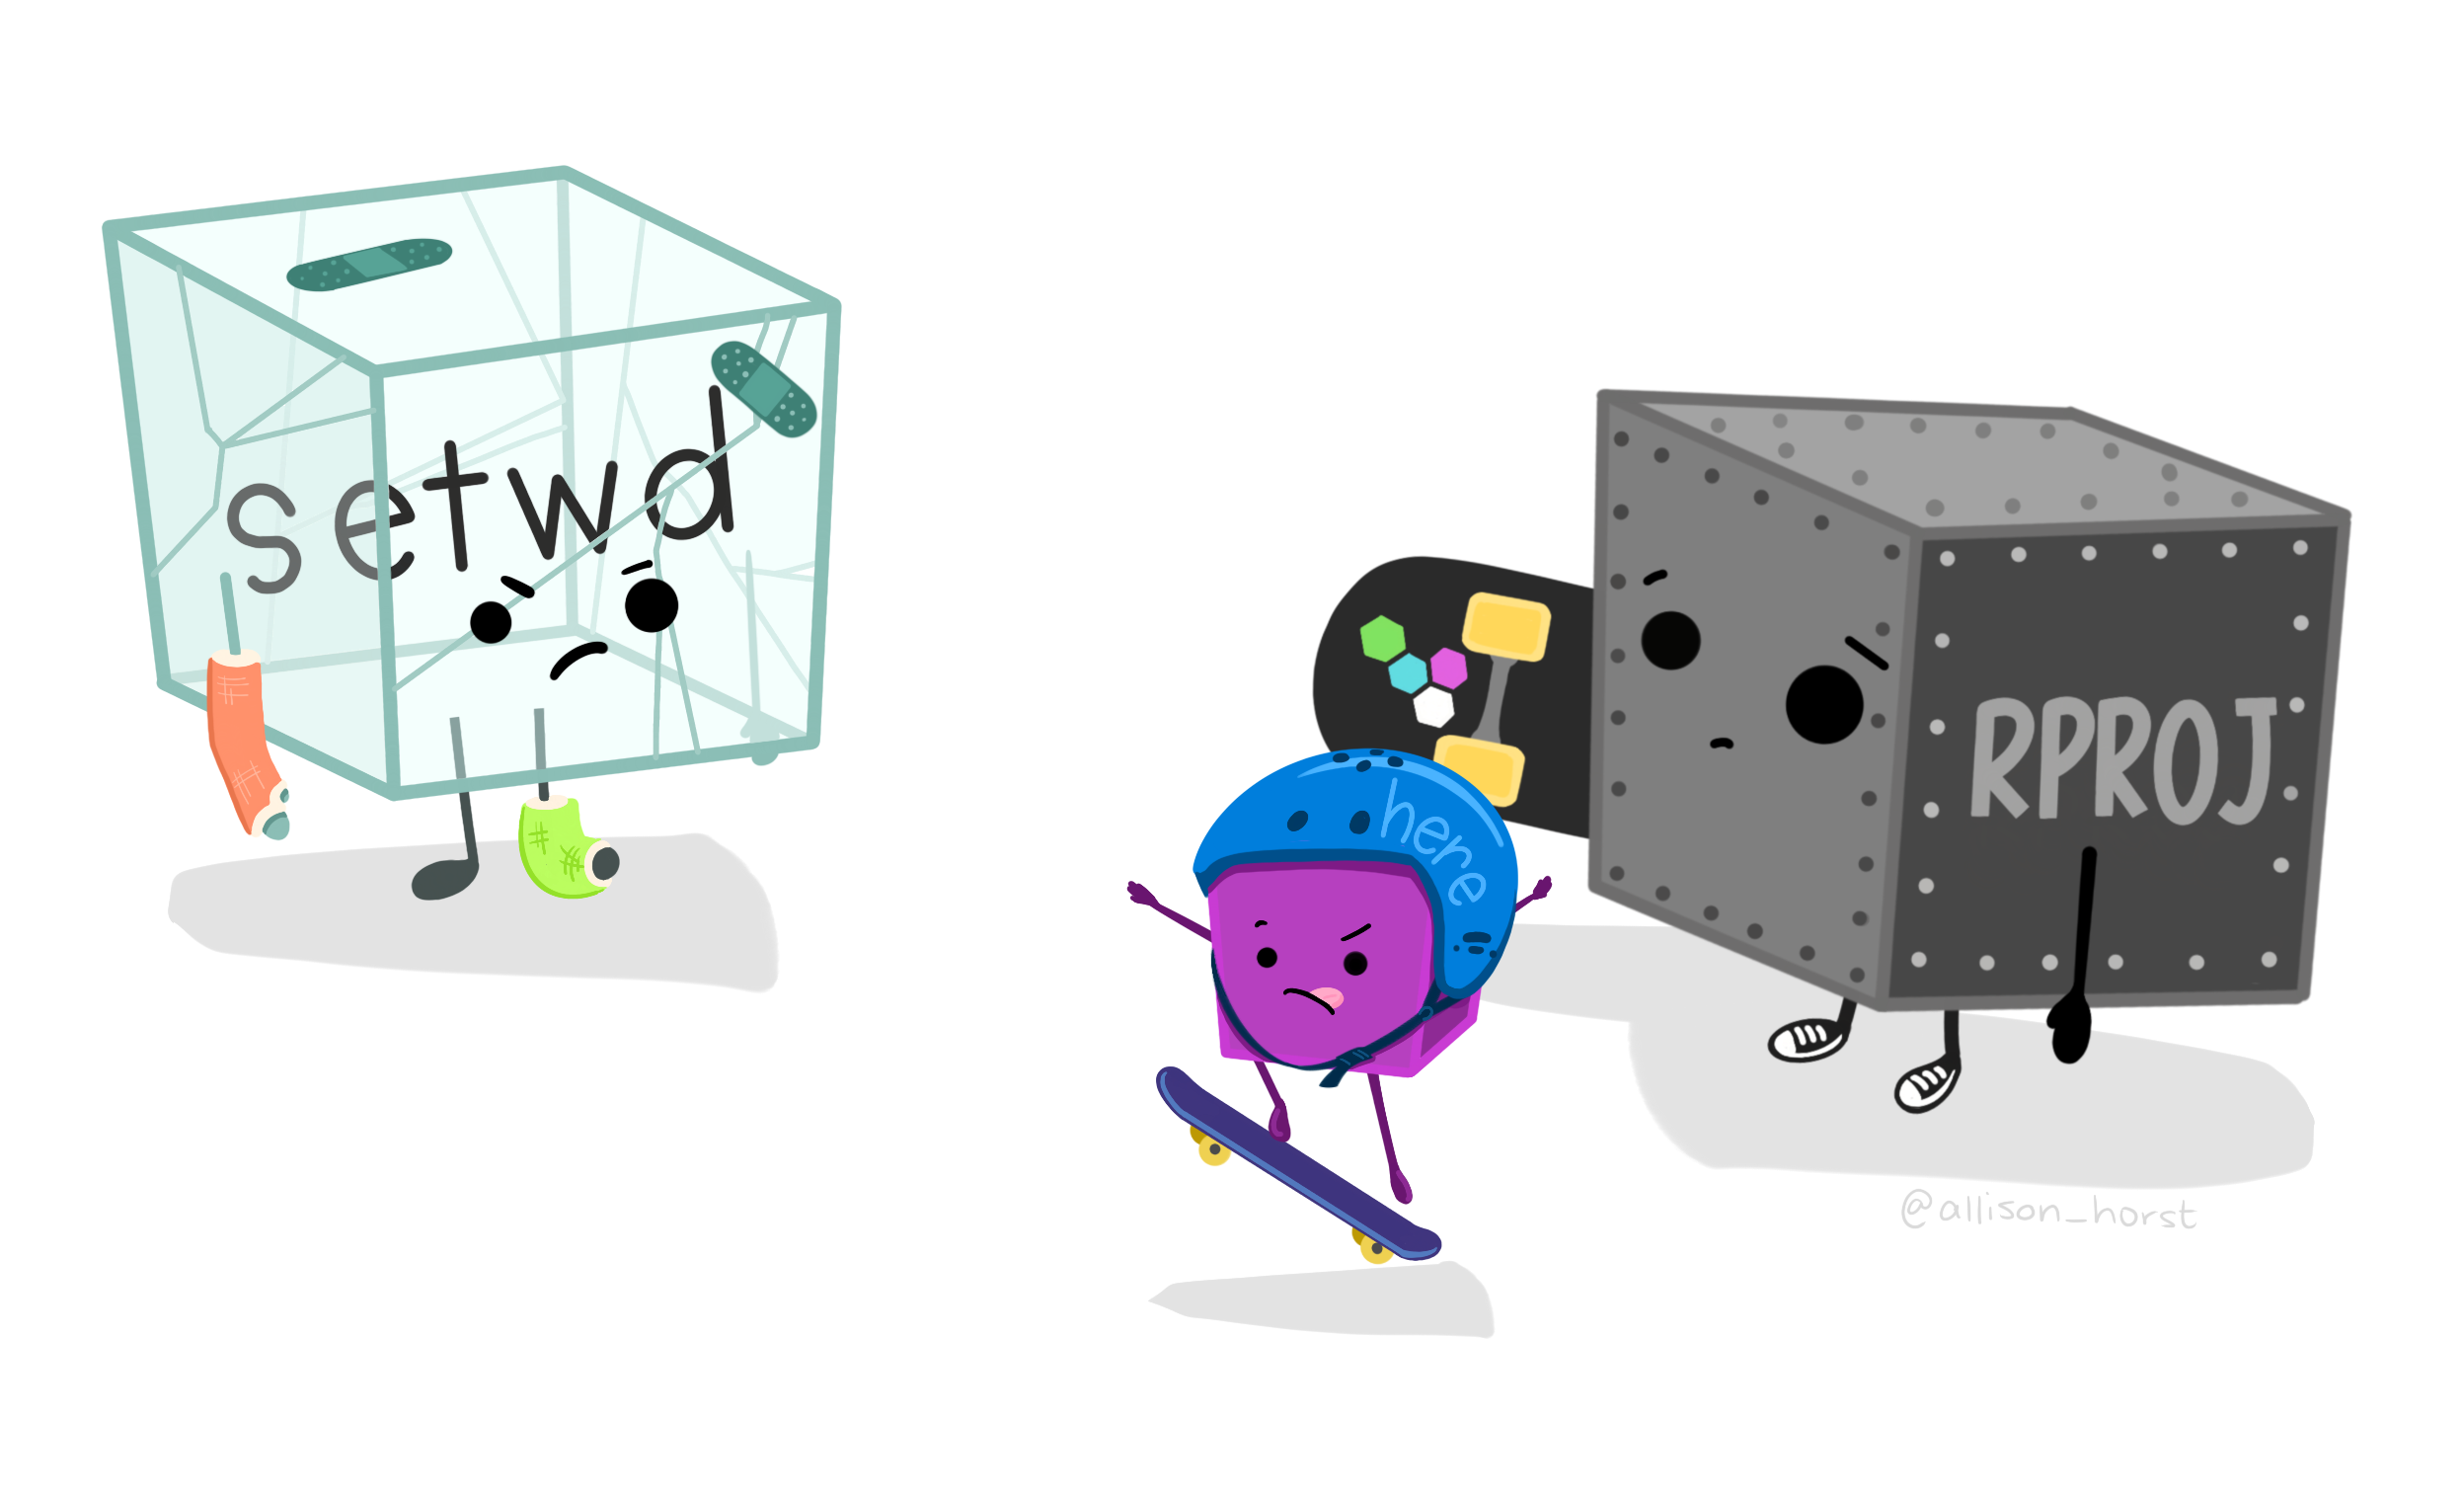
\includegraphics{img/cracked_setwd.png}

}

\subcaption{\label{fig-setwd}RStudio-Projekte sind viel sicherer als das
Arbeitsverzeichnis von Hand zu wählen oder mit Pfaden herumzubasteln.
Image credit: Allision Horst}

\end{minipage}%

\caption{\label{fig-projects}Nutzen Sie RStudio-Projekte, das macht Ihr
Leben leichter.}

\end{figure}%

\subsubsection{Skriptdateien}\label{skriptdateien}

Die R-Befehle (``Syntax'') schreiben Sie am besten in eine speziell
dafür vorgesehene Textdatei in RStudio. Eine Sammlung von
(R-)Computer-Befehlen nennt man auch ein \emph{Skript}, daher spricht
man auch von einer \emph{Skriptdatei}.

\paragraph{So öffnen Sie eine neue
Skriptdatei}\label{so-uxf6ffnen-sie-eine-neue-skriptdatei}

Um eine neue R-Skriptdatei zu öffnen, klicken Sie auf das Icon, das ein
weißes Blatt mit einem grünen Pluszeichen zeigt, s.
Figure~\ref{fig-script-new}.

\begin{figure}

\begin{minipage}{0.50\linewidth}

\centering{

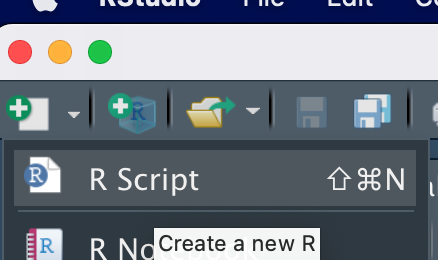
\includegraphics[width=0.5\textwidth,height=\textheight]{img/script-new.png}

}

\subcaption{\label{fig-script-new1}So erstellen Sie eine neue
Skriptdatei}

\end{minipage}%
%
\begin{minipage}{0.50\linewidth}
\end{minipage}%
\newline
\begin{minipage}{0.50\linewidth}
\end{minipage}%

\caption{\label{fig-script-new}Es gibt verschiedene Wege, um eine neue
R-Skript-Datei in RStudio zu öffnen.}

\end{figure}%

\paragraph{So speichern Sie Ihre
Skripdatei}\label{so-speichern-sie-ihre-skripdatei}

Vergessen Sie nicht zu \emph{speichern}, wenn Sie ein tolles Skript
geschrieben haben. Dafür gibt es mehrere Möglichkeiten:

\begin{enumerate}
\def\labelenumi{\arabic{enumi}.}
\tightlist
\item
  Tastaturkürzel \emph{Strg+S}
\item
  Menü: \texttt{File\ \textgreater{}\ Save}
\item
  Klick auf das Icon mit der Diskette, s. Figure~\ref{fig-script-new}.
\end{enumerate}

\paragraph{So öffnen Sie eine
Skriptdatei}\label{so-uxf6ffnen-sie-eine-skriptdatei}

Eine Skriptdatei können Sie in typischer Manier \emph{öffnen}:

\begin{enumerate}
\def\labelenumi{\arabic{enumi}.}
\tightlist
\item
  Strg+O
\item
  Klick auf das Icon mit der Akte und dem grünen Pfeil (vgl.
  Figure~\ref{fig-script-new})
\item
  Menü: \texttt{File\ \textgreater{}\ Open\ File...}
\end{enumerate}

\subsubsection{Quarto-Dokumente}\label{quarto-dokumente}

\href{https://quarto.org/}{Quarto} ist ein Programm zum Erstellen von
Texten, in das man R-Syntax einfügen kann. Die Ausgaben der R-Befehle
werden dann direkt im Dokument eingebunden. Figure~\ref{fig-exm-quarto}
zeit ein Beispiel für ein Quarto-Dokument.

\begin{tcolorbox}[enhanced jigsaw, coltitle=black, colframe=quarto-callout-note-color-frame, opacityback=0, toprule=.15mm, opacitybacktitle=0.6, arc=.35mm, titlerule=0mm, toptitle=1mm, title=\textcolor{quarto-callout-note-color}{\faInfo}\hspace{0.5em}{Note}, bottomtitle=1mm, leftrule=.75mm, breakable, rightrule=.15mm, colbacktitle=quarto-callout-note-color!10!white, bottomrule=.15mm, colback=white, left=2mm]

Quarto ist eine komfortable und leistungsfähige Methode, um Dokumente
mit R-Syntax zu schreiben. Sie sind aber nicht verpflichtet, Quarto zu
nutzen. Stattdessen können Sie Ihre Syntax auch in Skriptdateien
schreiben. \(\square\)

\end{tcolorbox}

\begin{figure}

\centering{

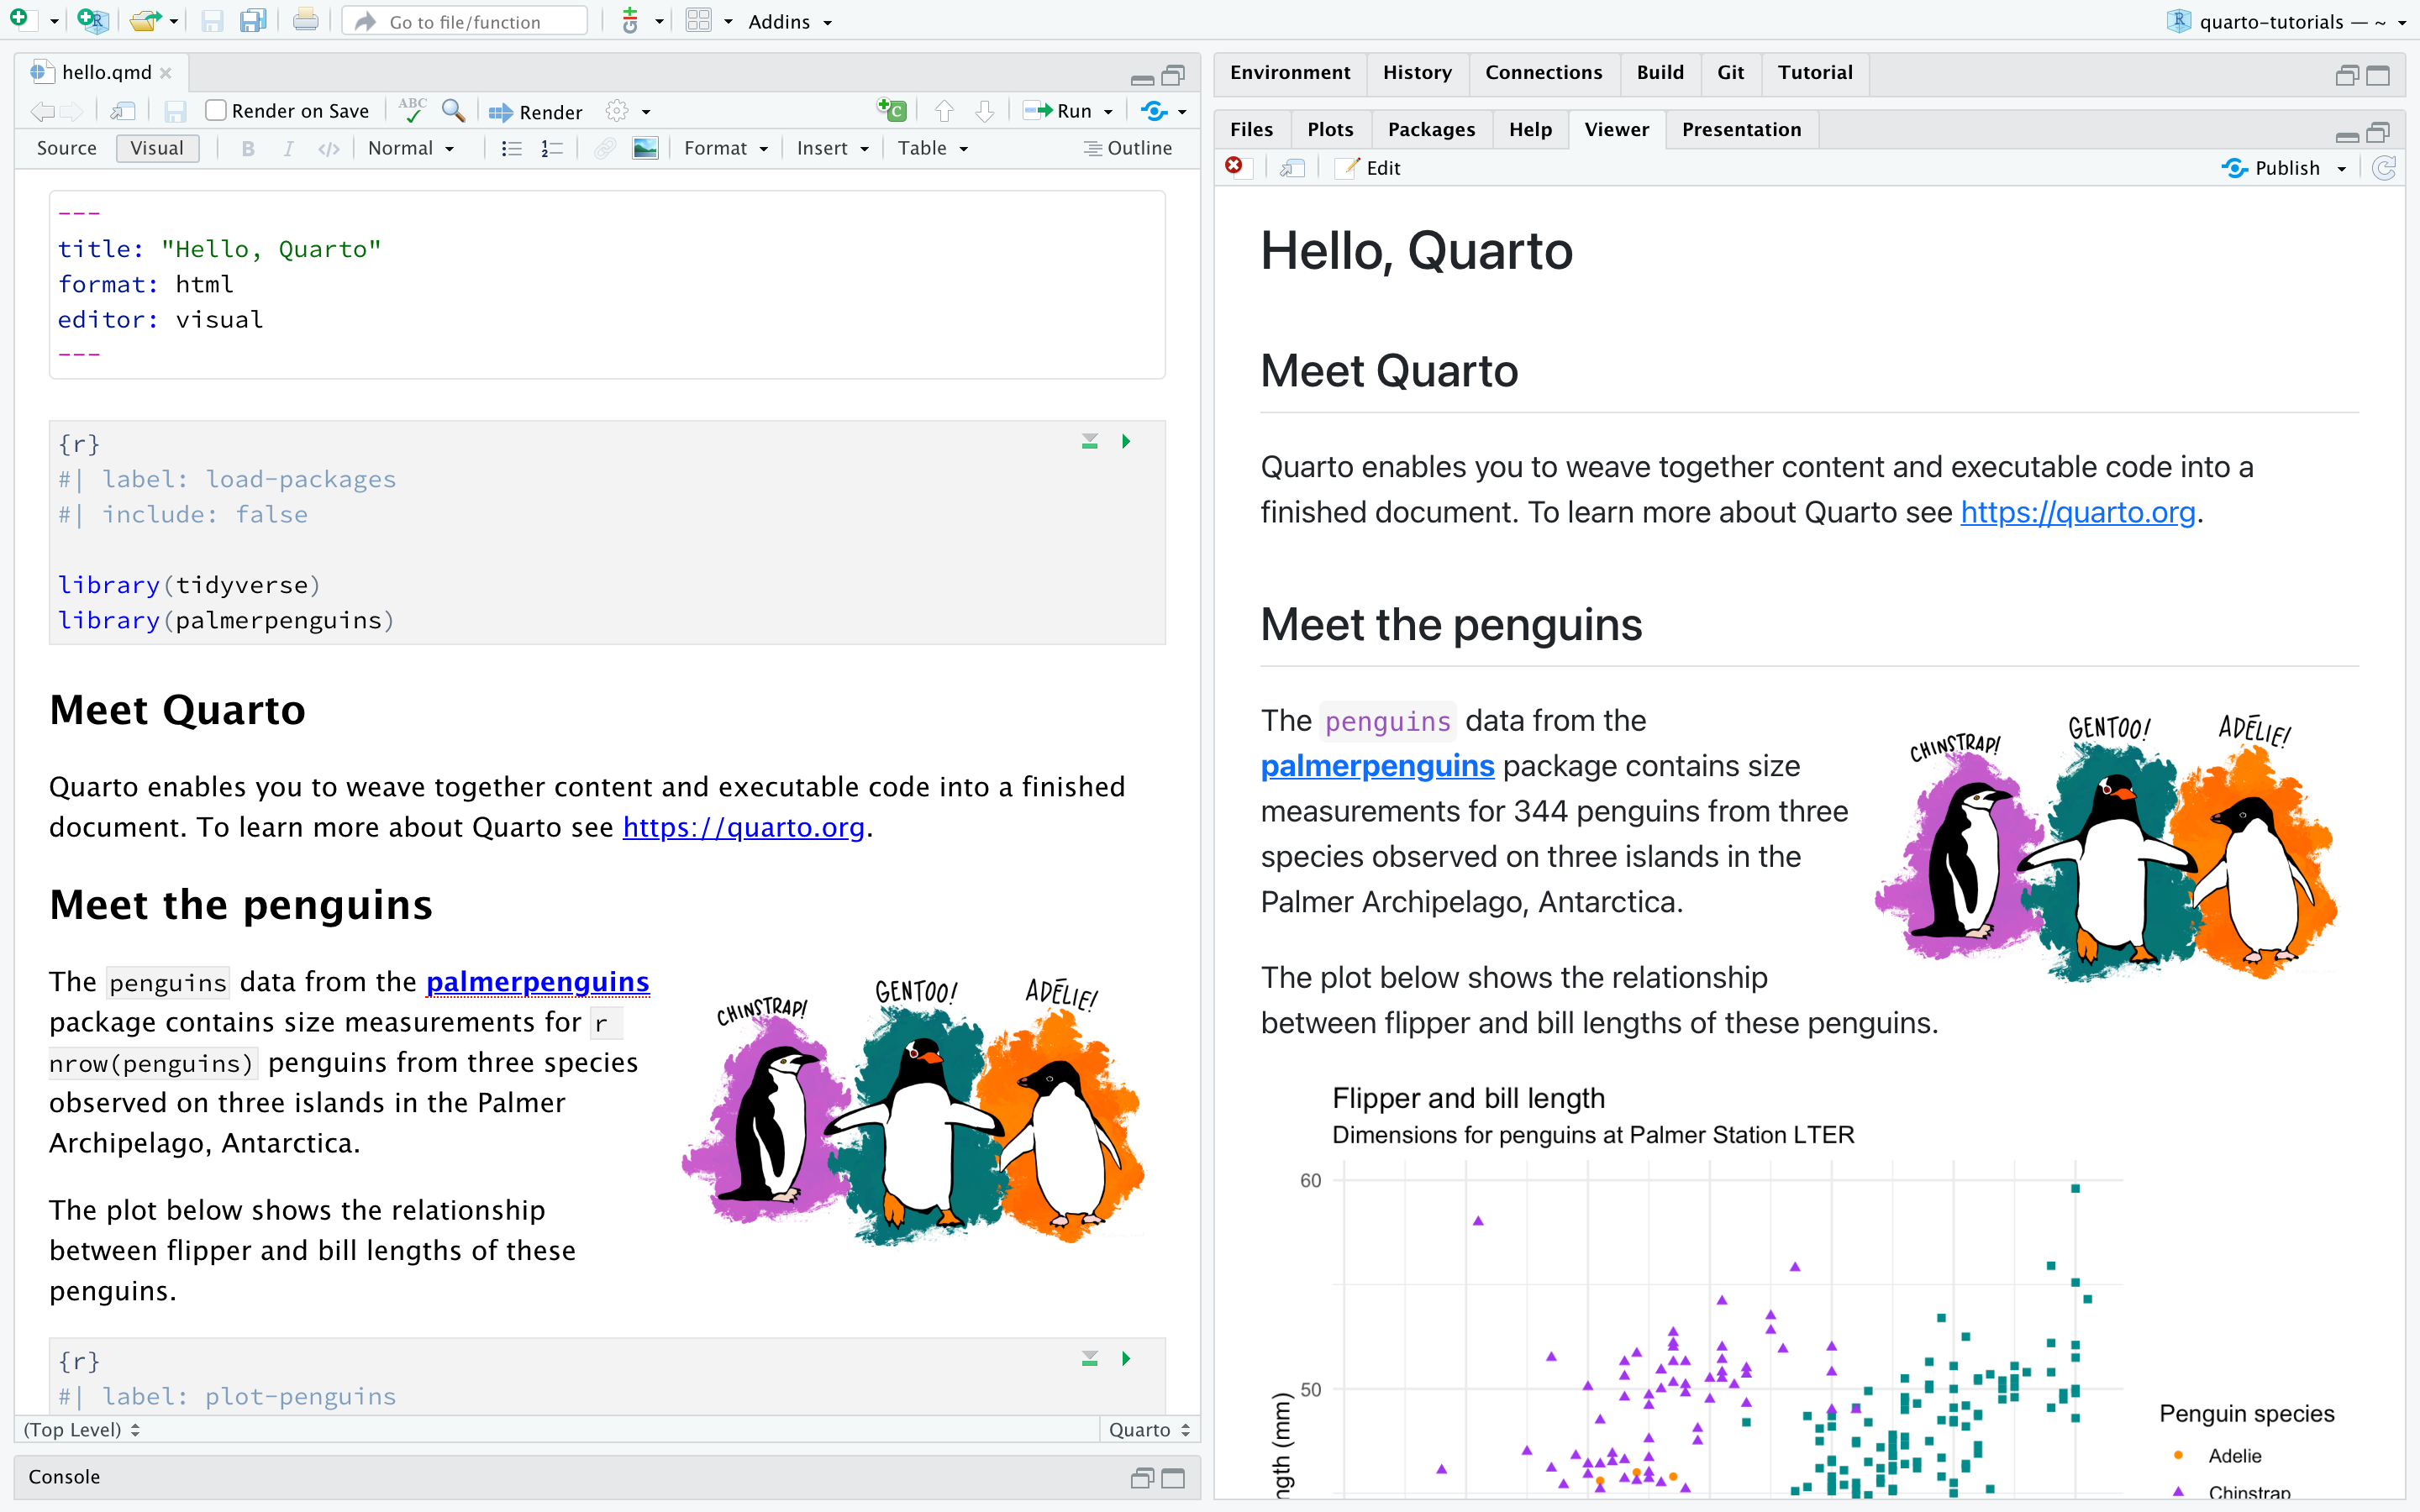
\includegraphics{020-R_files/mediabag/rstudio-hello.png}

}

\caption{\label{fig-exm-quarto}Dokumente schreiben mit Quarto}

\end{figure}%

Wenn Sie Quarto nutzen möchten, müssen Sie es zunächst installieren,
d.h. \href{https://quarto.org/docs/get-started/}{herunterladen}. Dann
können Sie in RStudio Quarto-Dateien erstellen.\footnote{\textless ttps://quarto.org/docs/get-started/\textgreater{}}
Ein neues Quarto-Dokument können Sie erstellen mit Klick auf \emph{File
\textgreater{} New File \textgreater{} Quarto Document
\ldots{}}.\footnote{Dieses Video \url{https://youtu.be/_f3latmOhew} gibt
  Ihnen Einstiegshilfe in Quarto.}

\subsection{Errisch für Einsteiger}\label{errisch-fuxfcr-einsteiger}

\begin{tcolorbox}[enhanced jigsaw, coltitle=black, colframe=quarto-callout-note-color-frame, opacityback=0, toprule=.15mm, opacitybacktitle=0.6, arc=.35mm, titlerule=0mm, toptitle=1mm, title=\textcolor{quarto-callout-note-color}{\faInfo}\hspace{0.5em}{Note}, bottomtitle=1mm, leftrule=.75mm, breakable, rightrule=.15mm, colbacktitle=quarto-callout-note-color!10!white, bottomrule=.15mm, colback=white, left=2mm]

Sie finden den R-Code für jedes Kapitel
\href{https://github.com/sebastiansauer/statistik1/tree/main/R-code-for-all-chapters}{hier}.
\(\square\)

\end{tcolorbox}

\subsubsection{Variablen}\label{sec-rvars}

In jeder Programmiersprache kann man Variablen definieren, so auch in R:

\begin{Shaded}
\begin{Highlighting}[]
\NormalTok{richtige\_antwort }\OtherTok{=} \DecValTok{42}
\NormalTok{falsche\_antwort }\OtherTok{=} \DecValTok{43}
\NormalTok{typ }\OtherTok{=} \StringTok{"Antwort"}
\NormalTok{ist\_korrekt }\OtherTok{=} \ConstantTok{TRUE}
\end{Highlighting}
\end{Shaded}

Alternativ zum Gleichheitszeichen \texttt{=} können Sie auch (synonym)
den Zuweisungspfeil \texttt{\textless{}-} verwenden. Beides führt zum
gleichen Ergebnis. Allerdings ist der Zuweisungspfeil präziser, und
sollte daher \emph{bevorzugt} werden.

Der \emph{Zuweisungspfeil} \texttt{\textless{}-} bzw. das
Gleichheitszeichen \texttt{=} definiert eine neue \emph{Variable} (oder
überschreibt den Inhalt, wenn die Variable schon existiert).\footnote{Dieses
  Video
  \url{https://www.youtube.com/watch?v=TKQk-tEF9YQ&list=PLRR4REmBgpIEaIyeNBgNGPgmhQJ_T1y8_&index=28}
  und dieses Video
  \url{https://www.youtube.com/watch?v=Nal0m_AmMwg&list=PLRR4REmBgpIEaIyeNBgNGPgmhQJ_T1y8_&index=48}
  geben eine Einführung in das Definieren von Variablen in R}.

\begin{Shaded}
\begin{Highlighting}[]
\NormalTok{richtige\_antwort }\OtherTok{\textless{}{-}} \DecValTok{42}
\NormalTok{falsche\_antwort }\OtherTok{\textless{}{-}} \DecValTok{43}
\NormalTok{typ }\OtherTok{\textless{}{-}} \StringTok{"Antwort"}
\NormalTok{ist\_korrekt }\OtherTok{\textless{}{-}} \ConstantTok{TRUE}
\end{Highlighting}
\end{Shaded}

Sie können sich eine Variable wie einen Becher oder Behälter vorstellen,
der bestimmte Werte enthält. Auf dem Becher steht (mit Edding
geschrieben) der Name des Bechers. Natürlich können Sie die Werte aus
dem Becher entfernen und sie durch neue ersetzen (vgl.
Figure~\ref{fig-def-vars}).

\begin{figure}

\centering{

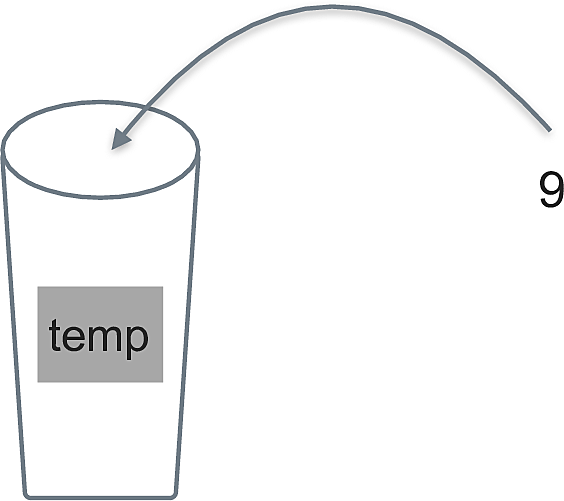
\includegraphics[width=0.25\textwidth,height=\textheight]{img/Variablen_zuweisen.png}

}

\caption{\label{fig-def-vars}Variablen zuweisen}

\end{figure}%

R kann übrigens auch rechnen. Probieren Sie es doch gleich mal hier aus!

\begin{Shaded}
\begin{Highlighting}[]
\NormalTok{die\_summe }\OtherTok{\textless{}{-}}\NormalTok{ falsche\_antwort }\SpecialCharTok{+}\NormalTok{ richtige\_antwort}
\end{Highlighting}
\end{Shaded}

Aber was ist jetzt der Wert, der ``Inhalt'' der Variable
\texttt{die\_summe}?

Um den Wert, d.h. den Inhalt einer Variablen in R \emph{auszulesen},
geben wir einfach den Namen des Objekts ein:

\begin{Shaded}
\begin{Highlighting}[]
\NormalTok{die\_summe}
\end{Highlighting}
\end{Shaded}

\begin{verbatim}
[1] 85
\end{verbatim}

Was passiert wohl, wenn wir \texttt{die\_summe} jetzt wie folgt
definieren?

\begin{Shaded}
\begin{Highlighting}[]
\NormalTok{die\_summe }\OtherTok{\textless{}{-}}\NormalTok{ falsche\_antwort }\SpecialCharTok{+}\NormalTok{ richtige\_antwort }\SpecialCharTok{+} \DecValTok{1}
\end{Highlighting}
\end{Shaded}

Wer hätt's geahnt:

\begin{Shaded}
\begin{Highlighting}[]
\NormalTok{die\_summe}
\end{Highlighting}
\end{Shaded}

\begin{verbatim}
[1] 86
\end{verbatim}

Variablen können auch ``leer'' sein:

\begin{Shaded}
\begin{Highlighting}[]
\NormalTok{alter }\OtherTok{\textless{}{-}} \ConstantTok{NA}
\NormalTok{alter}
\end{Highlighting}
\end{Shaded}

\begin{verbatim}
[1] NA
\end{verbatim}

\texttt{NA} steht für \emph{not available}, nicht verfügbar und macht
deutlich, dass hier ein Wert fehlt.

\begin{quote}
🧑‍🎓 Wozu brauche ich bitte fehlende Werte?!
\end{quote}

Fehlende Werte sind ein häufiges Problem in der Praxis. Vielleicht hat
sich die befragte Person geweigert, ihr Alter anzugeben\footnote{Datenschutz!}.
Oder als Sie die Daten in Ihren Computer eingeben wollten, ist Ihre
Katze über die Tastatur gelaufen und alles war futsch\ldots{}

\subsubsection{Funktionen (``Befehle'')}\label{funktionen-befehle}

Das, was R kann, ist in ``Funktionen'' hinterlegt. Genauer gesagt ist
``Befehl'' eine Funktion.

\begin{definition}[Funktion]\protect\hypertarget{def-fun}{}\label{def-fun}

Eine Funktion ist eine Regel, die jedem Eingabewert (auch Argument
genannt) einen Ausgabewert zuordnet. Man kann sich Funktionen als
Maschinen vorstellen, die Eingabedaten in Ausgabedaten umwandeln, vgl.
Figure~\ref{fig-function-schema}. \(\square\)

\end{definition}

\paragraph{Eine erste Funktion: Vektoren
erstellen}\label{eine-erste-funktion-vektoren-erstellen}

Ein Beispiel für eine solche Funktion könnte sein: ``Berechne den
Mittelwert dieser Datenreihe'' (schauen wir uns gleich an).

Das geht so:

\begin{Shaded}
\begin{Highlighting}[]
\NormalTok{Antworten }\OtherTok{\textless{}{-}} \FunctionTok{c}\NormalTok{(}\DecValTok{42}\NormalTok{, }\DecValTok{43}\NormalTok{)}
\end{Highlighting}
\end{Shaded}

Der Befehl \texttt{c} (c wie \emph{c}ombine) fügt mehrere Werte zusammen
zu einer ``Liste'' (einem Vektor).\footnote{Streng genommen sollte man
  nicht von einer Liste sprechen, da es in R noch einen anderen
  Objekttyp gibt, der \texttt{list} heißt, und eine verallgemeinerte
  Form eines Vektors ist.}

\begin{definition}[Vektor]\protect\hypertarget{def-vektor}{}\label{def-vektor}

Als \emph{Vektor} bezeichnen wir eine geordnete Folge von Werten. In R
kann man sie mit der Funktion \texttt{c()} erstellen. Die Werte eines
Vektors bezeichnet man als \emph{Elemente}. \(\square\)

\end{definition}

Mit dem Zuweisungspfeil geben wir diesem Vektor einen Namen, hier
\texttt{Antworten}. Dieser Vektor besteht aus zwei Werten, zuerst
\texttt{42}, dann kommt \texttt{43}.

\begin{example}[Beispiele für
Vektoren]\protect\hypertarget{exm-vektoren}{}\label{exm-vektoren}

Vektoren können (praktisch) beliebig lang sein, z.B. drei Elemente.

\begin{Shaded}
\begin{Highlighting}[]
\NormalTok{x }\OtherTok{\textless{}{-}} \FunctionTok{c}\NormalTok{(}\DecValTok{1}\NormalTok{, }\DecValTok{2}\NormalTok{, }\DecValTok{3}\NormalTok{)}
\NormalTok{y }\OtherTok{\textless{}{-}} \FunctionTok{c}\NormalTok{(}\DecValTok{2}\NormalTok{, }\DecValTok{1}\NormalTok{, }\DecValTok{3}\NormalTok{)  }\CommentTok{\# x und y sind ungleich (Reihenfolge der Werte)}
\NormalTok{z }\OtherTok{\textless{}{-}} \FunctionTok{c}\NormalTok{(}\FloatTok{3.14}\NormalTok{, }\FloatTok{2.71}\NormalTok{)  }
\NormalTok{namen }\OtherTok{\textless{}{-}} \FunctionTok{c}\NormalTok{(}\StringTok{"Anni"}\NormalTok{, }\StringTok{"Bert"}\NormalTok{, }\StringTok{"Charli"}\NormalTok{) }\CommentTok{\# Text{-}Vektor}
\end{Highlighting}
\end{Shaded}

\end{example}

Zwei wichtige Typen von Vektoren sind numerische Vektoren (reelle
Zahlen; in R auch als \emph{numeric} oder \emph{double} bezeichnet) und
Textvektoren, in R auch als \emph{String} oder \emph{character}
bezeichnet.

\begin{example}[]\protect\hypertarget{exm-funs}{}\label{exm-funs}

Weitere Beispiel für Funktionen sind:

\begin{itemize}
\tightlist
\item
  ``Erstelle eine Liste (Vektor) von Werten''.
\item
  ``Lade dieses R-Paket.''
\item
  ``Gib den größten Wert dieser Datenreihe aus.'' \(\square\)
\end{itemize}

\end{example}

\subsubsection{Unsere erste statistische Funktion}\label{sec-first-fun}

Jetzt wird's ernst. Jetzt kommt die Statistik. 🧟 Berechnen wir also
unsere erste statistische Funktion: Den Mittelwert. Puh.

\begin{Shaded}
\begin{Highlighting}[]
\FunctionTok{mean}\NormalTok{(Antworten)}
\end{Highlighting}
\end{Shaded}

\begin{verbatim}
[1] 42.5
\end{verbatim}

Sie hätten \texttt{Antworten} auch durch \texttt{c(42,\ 43)} ersetzen
können, so haben Sie ja schließlich die Variable gerade definiert.

R arbeitet so einen ``verschachtelten'' Befehl \emph{von innen nach
außen} ab:

Start: \texttt{mean(Antworten)}

{\(\downarrow\)}

Schritt 1: \texttt{mean(c(42,\ 43))}

{\(\downarrow\)}

Schritt 2: \texttt{42.5}

\paragraph{Schema einer Funktion}\label{schema-einer-funktion}

Figure~\ref{fig-function-schema} stellt eine Funktion schematisch dar.

\begin{figure}

\centering{

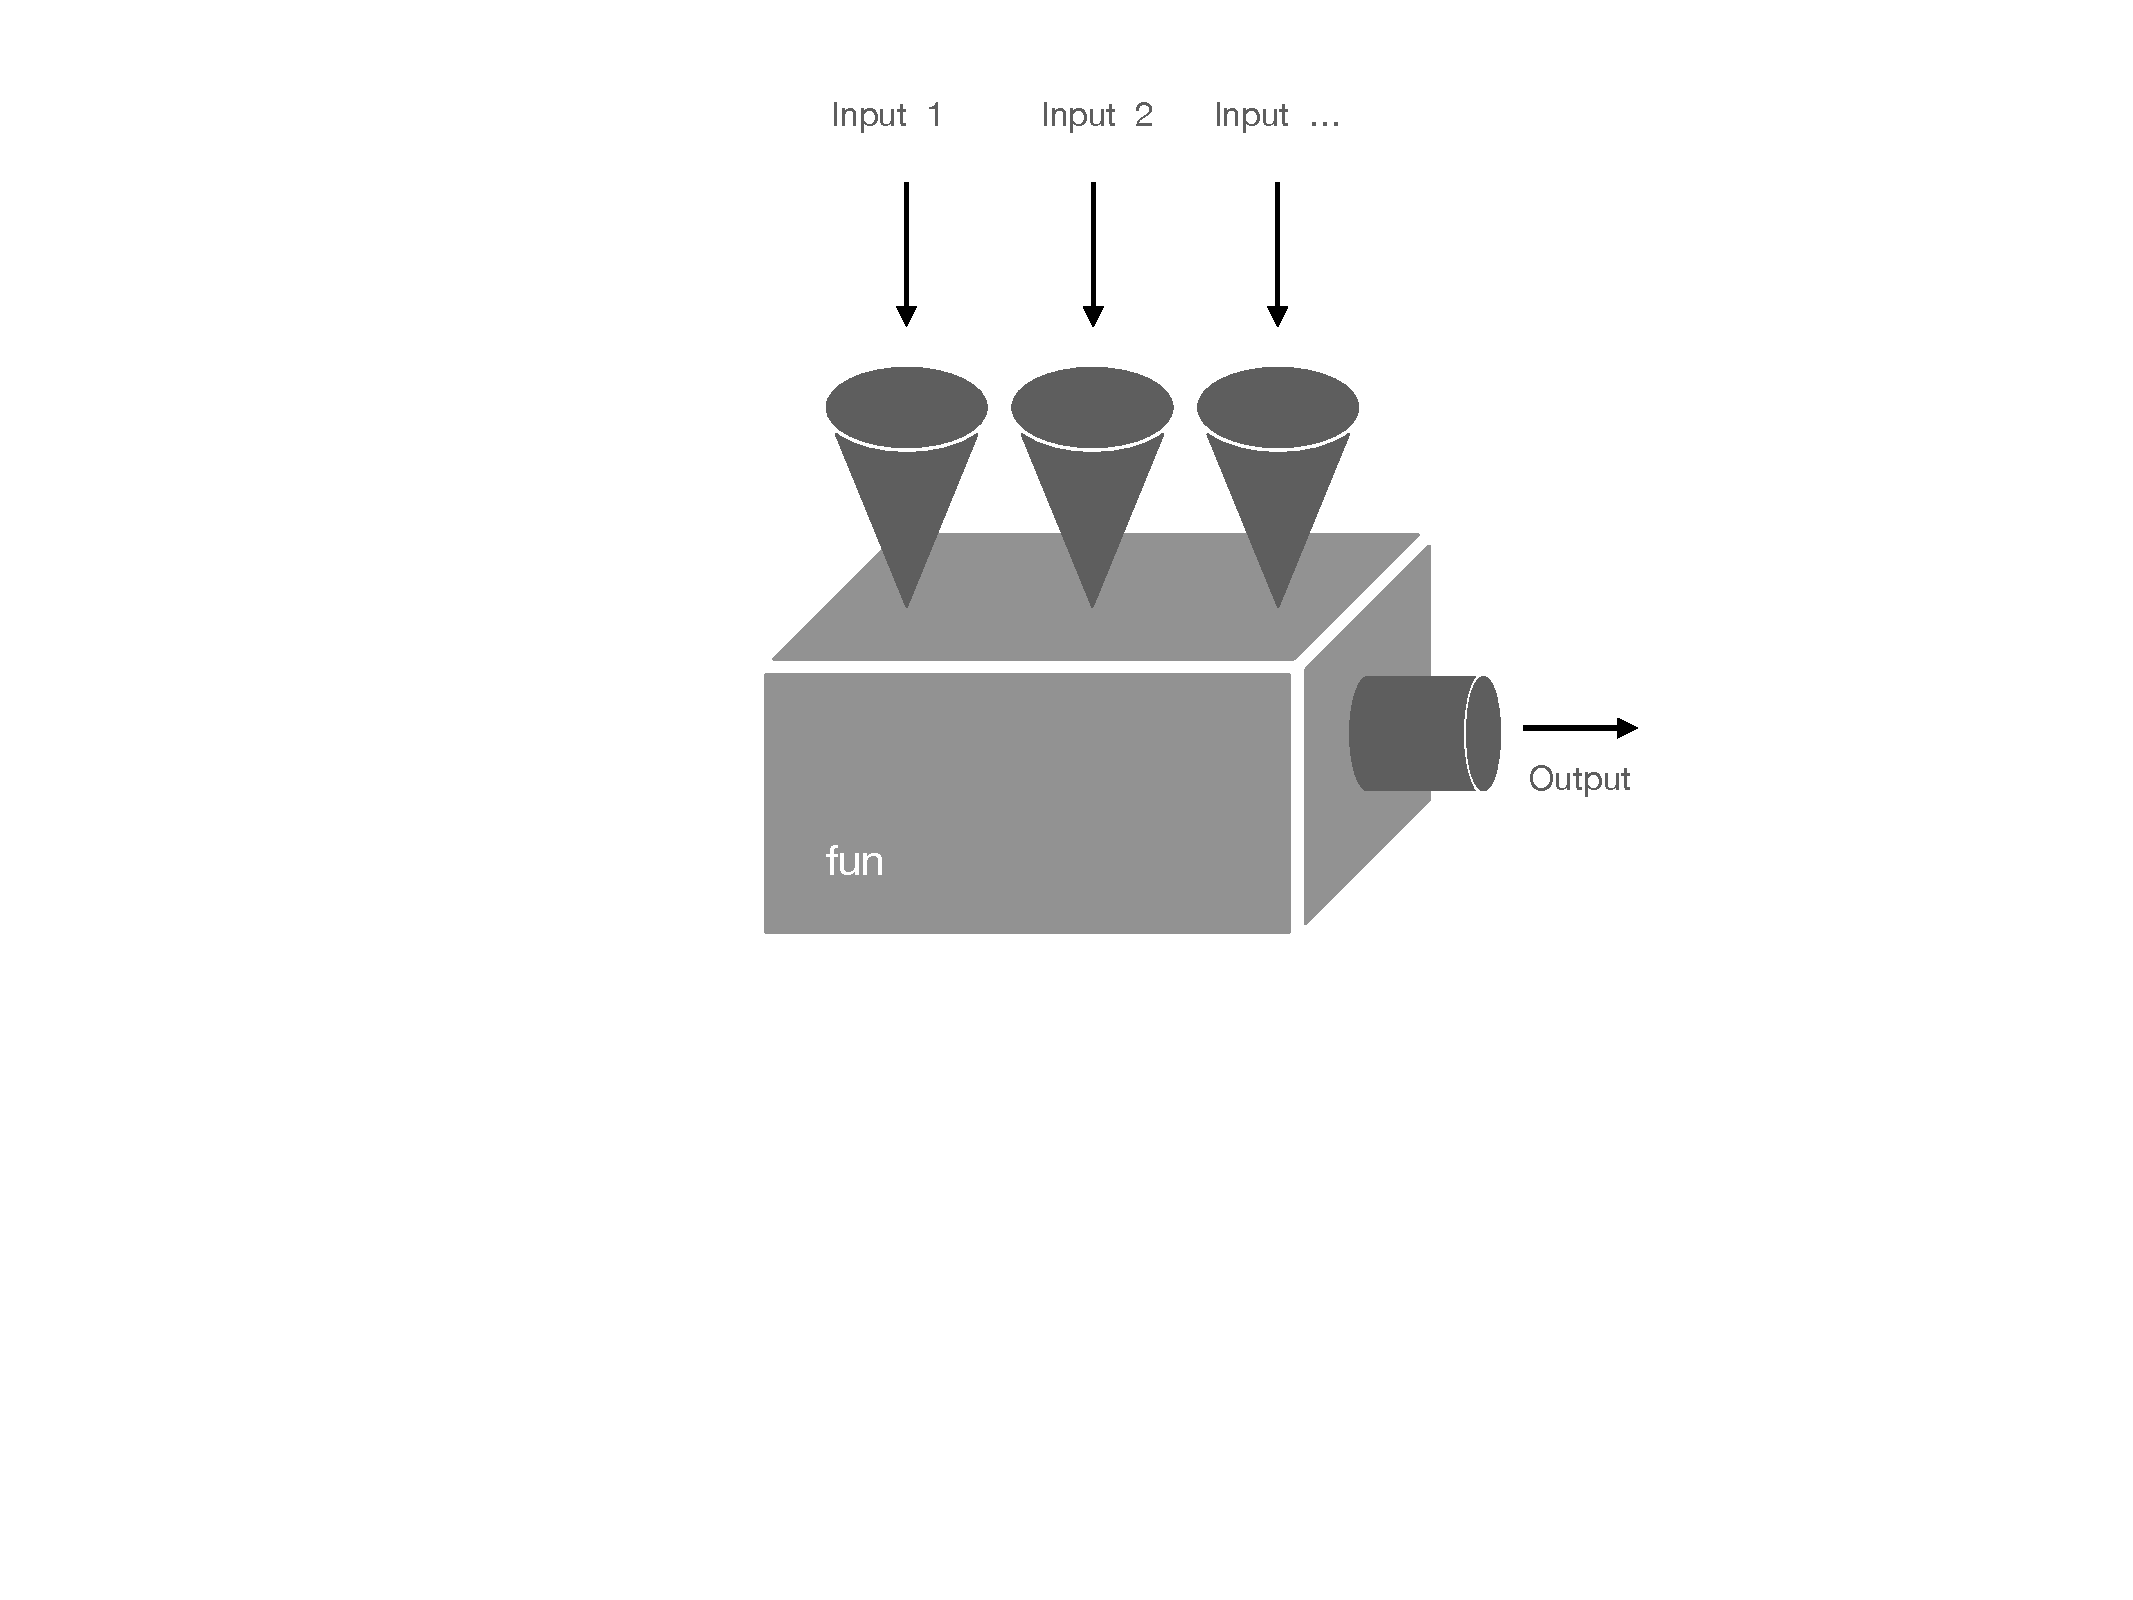
\includegraphics[width=0.5\textwidth,height=\textheight]{img/function-schema.pdf}

}

\caption{\label{fig-function-schema}Schema einer Funktion}

\end{figure}%

\paragraph{Argumente einer Funktion}\label{argumente-einer-funktion}

Eine Funktion hat einen oder mehrere \emph{Inputs} (s.
Figure~\ref{fig-function-schema}), das sind Daten oder
Verarbeitungshinweise, die man in die Funktion \texttt{fun}
\emph{eingibt}, bevor sie loslegt. Eine Funktion hat immer (genau) eine
\emph{Ausgabe} (Output), in der das Ergebnis einer Funktion ausgegeben
wird.

\begin{definition}[Argumente einer
Funktion]\protect\hypertarget{def-args}{}\label{def-args}

Die ``Trichter'' einer (R-)Funktion, in denen man die Eingaben
``einfüllt'', nennt man auch \emph{Argumente}.\(\square\)

\end{definition}

So hat die Funktion \texttt{mean()} z.B. folgende Argumente, s.
Listing~\ref{lst-mean}.

\begin{codelisting}

\caption{\label{lst-mean}Die Argumente der R-Funktion \texttt{mean}}

\centering{

\begin{Shaded}
\begin{Highlighting}[]
\FunctionTok{mean}\NormalTok{(x, }\AttributeTok{trim =} \DecValTok{0}\NormalTok{, }\AttributeTok{na.rm =} \ConstantTok{FALSE}\NormalTok{, ...)}
\end{Highlighting}
\end{Shaded}

}

\end{codelisting}%

\begin{itemize}
\tightlist
\item
  \texttt{x}: das ist der Vektor, für den der Mittelwert berechnet
  werden soll
\item
  \texttt{trim\ =\ 0}: Sollen die extremsten Werte von \texttt{x} lieber
  ``abgeschnitten'' werden, also nicht in die Berechnung des Mittelwerts
  einfließen?
\item
  \texttt{na.rm\ =\ FALSE}: Wie soll mit fehlenden Werten \texttt{NA}
  umgegangen werden? Im Standard liefert \texttt{mean}\footnote{und
    viele andere arithmetische Funktionen in R} \texttt{NA} zurück. R
  schwenkt sozusagen die rote Fahne, um zu signalisieren, Achtung,
  Mensch, hier ist irgendwas nicht in Ordnung. Setzt man aber
  \texttt{na.rm\ =\ TRUE}, dann entfernt (remove, rm) R die fehlenden
  Werte und berechnet den Mittelwert.
\item
  \texttt{...} heißt ``sonstiges Zeugs, das manchmal eine Rolle spielen
  könnte''; darum kümmern wir uns jetzt nicht.
\end{itemize}

Einige Argumente haben einen \emph{Standardwert} bzw. eine
\emph{Voreinstellung} (engl. \emph{default}). So wird bei der Funktion
\texttt{mean} im Standard nicht getrimmt (\texttt{trim\ =\ 0}) und
fehlende Werte werden nicht entfernt (\texttt{na.rm\ =\ FALSE)}.

\begin{tcolorbox}[enhanced jigsaw, coltitle=black, colframe=quarto-callout-note-color-frame, opacityback=0, toprule=.15mm, opacitybacktitle=0.6, arc=.35mm, titlerule=0mm, toptitle=1mm, title=\textcolor{quarto-callout-note-color}{\faInfo}\hspace{0.5em}{Note}, bottomtitle=1mm, leftrule=.75mm, breakable, rightrule=.15mm, colbacktitle=quarto-callout-note-color!10!white, bottomrule=.15mm, colback=white, left=2mm]

Wenn ein R-Befehl ein Argument mit Voreinstellung hat, brauchen Sie
dieses Argument \emph{nicht} zu befüllen. In dem Fall wird auf den Wert
der Voreinstellung zurückgegriffen. Argumente ohne Voreinstellung - wie
\texttt{x} bei \texttt{mean()} - müssen Sie aber auf jeden Fall mit
einem Wert befüllen. Man würde also \texttt{mean} zumeist so aufrufen:
\texttt{mean(x)}. \(\square\)

\end{tcolorbox}

Bei jedem R-Befehl haben die Argumente eine bestimmte Reihenfolge, etwa
bei \texttt{mean()}:
\texttt{mean(x,\ trim\ =\ 0,\ na.rm\ =\ FALSE,\ ...)}.

(Nur) wenn man die Argumente in ihrer vorgegebenen Reihenfolge
anspricht, muss man \emph{nicht} den Namen des Arguments anführen:

\emoji{check-mark-button} \texttt{mean(Antworten,\ 0,\ FALSE)}

Hält man sich aber nicht an die vorgebene Reihenfolge, so weiß R nicht,
was zu tun ist und flüchtet sich in eine Fehlermeldung:

\begin{Shaded}
\begin{Highlighting}[]
\FunctionTok{mean}\NormalTok{(Antworten, }\ConstantTok{FALSE}\NormalTok{, }\DecValTok{0}\NormalTok{)  }\CommentTok{\# FALSCH, DON\textquotesingle{}T DO IT }
\end{Highlighting}
\end{Shaded}

\begin{verbatim}
Error in mean.default(Antworten, FALSE, 0): 'trim' must be numeric of length one
\end{verbatim}

Wenn man die Namen der Argumente anspricht, ist die Reihenfolge egal:

\begin{Shaded}
\begin{Highlighting}[]
\FunctionTok{mean}\NormalTok{(}\AttributeTok{na.rm =} \ConstantTok{FALSE}\NormalTok{, }\AttributeTok{x =}\NormalTok{ Antworten)  }\CommentTok{\# ok}
\FunctionTok{mean}\NormalTok{(}\AttributeTok{trim =} \DecValTok{0}\NormalTok{, }\AttributeTok{x =}\NormalTok{ Antworten, }\AttributeTok{na.rm =} \ConstantTok{TRUE}\NormalTok{)  }\CommentTok{\# ok}
\end{Highlighting}
\end{Shaded}

Übrigens: Leerzeichen sind R fast immer egal. Aus Gründen der
Übersichtlichkeit sollte man aber Leerzeichen verwenden. In diesen
Fällen sind Leerzeichen nicht erlaubt:

\begin{itemize}
\tightlist
\item
  \texttt{\textless{}-}
\item
  \texttt{\textless{}=} etc.
\item
  Variablennamen
\end{itemize}

\paragraph{Achtung bei fehlenden
Werten}\label{achtung-bei-fehlenden-werten}

Sagen wir, wir haben einen fehlenden Wert in unseren Daten:

\begin{Shaded}
\begin{Highlighting}[]
\NormalTok{Antworten }\OtherTok{\textless{}{-}} \FunctionTok{c}\NormalTok{(}\DecValTok{42}\NormalTok{, }\DecValTok{43}\NormalTok{, }\ConstantTok{NA}\NormalTok{)}
\NormalTok{Antworten}
\end{Highlighting}
\end{Shaded}

\begin{verbatim}
[1] 42 43 NA
\end{verbatim}

Wenn wir jetzt den Mittelwert berechnen wollen, quittiert R das mit
einem schnöden \texttt{NA}. \texttt{NA} steht für \emph{not available},
ist also ein Hinweis, dass Werte fehlen.

\begin{Shaded}
\begin{Highlighting}[]
\FunctionTok{mean}\NormalTok{(Antworten)}
\end{Highlighting}
\end{Shaded}

\begin{verbatim}
[1] NA
\end{verbatim}

R meint es gut mit Ihnen\footnote{\textgreater{} Naja, manchmal.}.
Stellen Sie sich vor, dass R Sie auf dieses Problem aufmerksam machen
möchte:

\begin{quote}
Achtung, lieber Herr und Gebieter, du hast nicht mehr alle Latten am
Zaun, will sagen, alle Daten im Vektor!
\end{quote}

(Danke, R.)

Möchten Sie aber lieber R dieses Verhalten austreiben, so befüllen Sie
das Argument \texttt{na.rm} mit dem Wert \texttt{TRUE}.\footnote{\texttt{na.rm}
  steht für \emph{r}e\emph{m}ove die NA, also fehlenden Werte}

\begin{Shaded}
\begin{Highlighting}[]
\FunctionTok{mean}\NormalTok{(Antworten, }\AttributeTok{na.rm =} \ConstantTok{TRUE}\NormalTok{)}
\end{Highlighting}
\end{Shaded}

\begin{verbatim}
[1] 42.5
\end{verbatim}

\begin{exercise}[Geben Sie neue Bedeutungen an, was ``NA'' noch bedeuten
könnte!]\protect\hypertarget{exr-na}{}\label{exr-na}

~

\begin{quote}
Wie wäre es mit ``nebulöse Anomalie'' oder ``nix-checkender Angeber''
oder ``nölender Automat''.
\end{quote}

\begin{quote}
Hm\ldots{}
\end{quote}

\(\square\)

\end{exercise}

\subsubsection{Vektorielles Rechnen}\label{sec-veccalc}

\begin{definition}[Vektorielles
Rechnen]\protect\hypertarget{def-veccalc}{}\label{def-veccalc}

Das Rechnen mit Vektoren in R bezeichnen wir als \emph{vektorielles
Rechnen}. \(\square\)

\end{definition}

Vektorielles Rechnen ist ein praktische Angelegenheit, man kann z.B.
folgende Dinge einfach in R ausrechnen.

Gegeben sei \texttt{x} als Vektor \texttt{(1,\ 2,\ 3)}. Dann können wir
die Differenz (Abweichung) jedes Elements von \texttt{x} zum Mittelwert
von \texttt{x} komfortabel so ausrechnen:

\begin{Shaded}
\begin{Highlighting}[]
\NormalTok{x }\SpecialCharTok{{-}} \FunctionTok{mean}\NormalTok{(x)}
\end{Highlighting}
\end{Shaded}

\begin{verbatim}
[1] -1  0  1
\end{verbatim}

Etwas fancier ausgedrückt: Wir haben die Funktion mit Namen
``Differenz'' (``Minus-Rechnen'') auf jedes Element von \texttt{x}
angewandt. Im Einzelnen haben wir also folgenden drei Differenzen
ausgerechnet:

\begin{Shaded}
\begin{Highlighting}[]
\DecValTok{1} \SpecialCharTok{{-}} \DecValTok{2}
\DecValTok{2} \SpecialCharTok{{-}} \DecValTok{2}
\DecValTok{3} \SpecialCharTok{{-}} \DecValTok{2}
\end{Highlighting}
\end{Shaded}

Diese drei Rechenschritte sind symbolisch in Figure~\ref{fig-vektoriell}
dargestellt.

\begin{figure}

\centering{

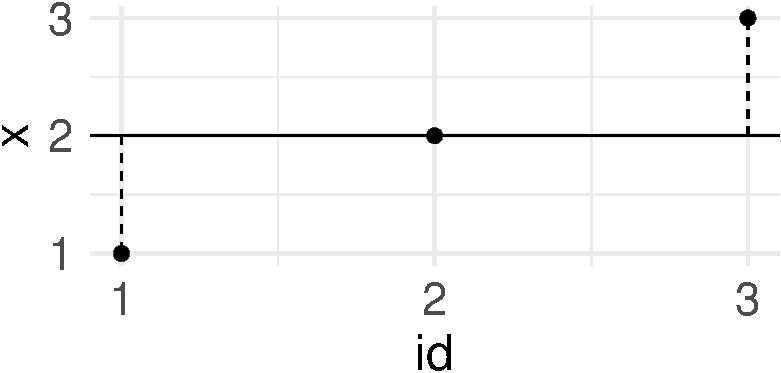
\includegraphics[width=0.5\textwidth,height=\textheight]{020-R_files/figure-pdf/fig-vektoriell-1.pdf}

}

\caption{\label{fig-vektoriell}Schema des vektoriellen Rechnens: Eine
Funktion wird auf jedes Element eines Vektors angewandt. Hier: 1-2=-1;
2-2=0; 3-2=1}

\end{figure}%

\subsubsection{R-Quiz}\label{r-quiz}

\begin{exercise}[]\protect\hypertarget{exr-rquiz}{}\label{exr-rquiz}

Ihre R-Muskeln sind gestählt? Oder doch noch nicht so ganz ausdefiniert?
{[}😤{]}\{\{.content-visible when-format=``html''\}\} Macht nichts!
Trainieren Sie sich mit dem R-Quiz auf der
Datenwerk-Webseite\footnote{\url{https://datenwerk.netlify.app/posts/r-quiz/r-quiz}}!
\(\square\)

\end{exercise}

\subsubsection{Ich brauche R-Hilfe!}\label{r-faq}

\begin{itemize}
\tightlist
\item
  \emph{Wo finde ich Hilfe zu einer bestimmten Funktion, z.B.
  \texttt{fun()}?} Geben Sie dazu folgenden R-Befehl ein:
  \texttt{help(fun)}. Alternativ geben Sie den Namen der Funktion in
  RStudio im Suchfeld beim Reiter \texttt{Help} ein.
\item
  \emph{Wenn ich ein R-Paket installiere, fragt mich R manchmal, ob ich
  auch Pakete installieren, will, die ``kompiliert'' werden müssen. Soll
  ich das machen?}. Nein, das ist nicht nötig; geben Sie ``no'' ein.
\item
  \emph{In welchem Paket wohnt meine R-Funktion}? Suchen Sie nach der
  Funktion auf der Webseite \emph{RDocumentation}\footnote{https://www.rdocumentation.org/}.
\item
  \emph{Ich weiß nicht, wie der R-Befehl funktioniert!} Vermutlich haben
  andere Ihr Problem auch, und meistens hat irgendwer das Problem schon
  gelöst. Am besten suchen Sie mal auf Stackoverflow\footnote{\url{https://www.stackoverflow.com}}.
\item
  \emph{Ich muss mal grundlegend verstehen, wozu ein bestimmten R-Paket
  gut ist. Was tun?} Lesen Sie die Dokumenation (``Vignette'') eines
  R-Pakets durch. Für das Paket \texttt{dplyr} bekommen Sie so einen
  Überblick über die verfügbaren Vignetten diese Pakets:
  \texttt{vignette(package\ =\ "dplyr")}. Dann suchen Sie sich aus der
  angezeigten Liste eine Vignette raus; mit \texttt{vignette("rowwise")}
  können Sie sich dann die gewünschte Vignette (z.B. \texttt{rowwise})
  anzeigen lassen.
\item
  \emph{Oh nein, ich seh rot, das heißt, R zeigt mir irgendwas in roter
  Schrift an. Ist jetzt was kaputt?} Keine Sorge, R ist in seiner
  Ausgabe nicht sparsam mit roter Frabe. Solange es nicht als
  Fehlermeldung (\texttt{ERROR}) erscheint, ist es meist kein Problem.
\item
  \emph{R hat sich aufgehängt oder bringt einen Fehler an einer Stelle,
  wo sonst alles funktioniert hat.} Probieren Sie auf jeden Fall mal das
  AEG-Prinzip (Aus-Ein-Gut): sprich R neu starten.
\item
  \emph{Ich suche schon seit einer Stunde einen Fehler und find ihn
  nicht. Ich habe schon verschiedene Gegenstände vor Wut an die Wand
  geworfen. Was soll ich tun?} Machen Sie eine Pause. Doch, das ist
  ernst gemeint. Meine Erfahrung: Mit etwas Abstand wird der Kopf klarer
  und man findet das Problem viel einfacher.\footnote{Und manchmal ist
    einem das Problem danach schlichtweg egal.}
\item
  \emph{Irgendwie reagiert R komisch, vielleicht hat es sich
  aufgehängt?} Starten Sie R neu. Klicken Sie auf \emph{Session
  \textgreater{} Restart R}.
\item
  \emph{Ich muss mal klar Schiff machen und alle (oder einige) Variablen
  löschen. Wie werd ich das Zeug wieder los?} Beim Neustart von R werden
  alle Objekte (Variablen) gelöscht. Einzelne Objekte können Sie
  selektiv löschen mit dem Befehl \texttt{rm}, so löscht
  \texttt{rm(mariokart)} das Objekt namens \texttt{mariokart}.
\end{itemize}

\begin{tcolorbox}[enhanced jigsaw, coltitle=black, colframe=quarto-callout-caution-color-frame, opacityback=0, toprule=.15mm, opacitybacktitle=0.6, arc=.35mm, titlerule=0mm, toptitle=1mm, title=\textcolor{quarto-callout-caution-color}{\faFire}\hspace{0.5em}{Caution}, bottomtitle=1mm, leftrule=.75mm, breakable, rightrule=.15mm, colbacktitle=quarto-callout-caution-color!10!white, bottomrule=.15mm, colback=white, left=2mm]

R ist penibel: So sind \texttt{name} und \texttt{Name} zwei verschiedene
Variablen für R. Groß- und Kleinschreibung wird von R streng beachtet!
Hingegen ist es R egal, ob Sie zur besseren Übersichtlichkeit
Leerzeichen in Ihre Syntax tippen. Ausnahme sind spezielle Operatoren
wie \texttt{\textless{}-} oder \texttt{\textless{}=}.

Eine gute Nachricht: Wenn R etwas von \texttt{WARNING} (bzw. Warnung)
sagt, können Sie das zumeist ignorieren. Eine \emph{Warnung} ist kein
Fehler (\texttt{ERROR}) und meistens nicht gravierend oder nicht
dringend. Ihre Syntax läuft trotzdem durch. Im Zweifel ist Googeln eine
gute Idee. Nur wenn R von \texttt{Error} spricht, ist es auch ein Fehler
und Ihre Syntax läuft nicht durch.\(\square\)

\end{tcolorbox}

\subsection{Mit Daten arbeiten}\label{mit-daten-arbeiten}

\subsubsection{Wo sind meine Daten?}\label{wo-sind-meine-daten}

Damit Sie eine Datendatei importieren können, müssen Sie wissen, wo die
Datei ist. Schauen wir uns zwei Möglichkeiten an, wo Ihre Datei liegen
könnte.

\begin{enumerate}
\def\labelenumi{\arabic{enumi}.}
\tightlist
\item
  Irgendwo im Internet\footnote{z.B. hier:
    \url{https://vincentarelbundock.github.io/Rdatasets/csv/openintro/mariokart.csv}}
\item
  Irgendwo auf Ihrem Computer, z.B. in Ihrem R-Projektordner
\end{enumerate}

In beiden Fällen wird der ``Aufenthaltsort'' der Datei durch den
\emph{Pfad}\footnote{Der Pfad einer Datei sagt, in welchem Ordner und
  Unterorder und Unter-Unterordner die gesuchte Datei liegt. Ein Pfad
  könnte z.B. so aussehen:
  ``/Users/sebastiansaueruser/github-repos/statistik1/''.} und den Namen
der Datei definiert.

\begin{tcolorbox}[enhanced jigsaw, coltitle=black, colframe=quarto-callout-note-color-frame, opacityback=0, toprule=.15mm, opacitybacktitle=0.6, arc=.35mm, titlerule=0mm, toptitle=1mm, title=\textcolor{quarto-callout-note-color}{\faInfo}\hspace{0.5em}{Note}, bottomtitle=1mm, leftrule=.75mm, breakable, rightrule=.15mm, colbacktitle=quarto-callout-note-color!10!white, bottomrule=.15mm, colback=white, left=2mm]

Wir werden in diesem Kurs häufiger mit dem Daten \texttt{mariokart}
arbeiten; Sie finden ihn
\href{https://vincentarelbundock.github.io/Rdatasets/csv/openintro/mariokart.csv}{hier}.\footnotemark{}

\end{tcolorbox}

\footnotetext{Auf dieser Webseite
\url{https://vincentarelbundock.github.io/Rdatasets/articles/data.html}
finden Sie eine große Zahl an Datensätzen. Nur für den Fall, dass Ihnen
langweilig ist.}

\subsubsection{Gebräuchliche
Datenformate}\label{gebruxe4uchliche-datenformate}

Daten werden in verschiedenen Formaten im Computer abgespeichert;
Tabellen häufig als

\begin{itemize}
\tightlist
\item
  Excel-Datei
\item
  CSV-Datei
\end{itemize}

In der Datenanalyse ist das gebräuchlichste Format für Daten in
Tabellenform die \emph{CSV-Datei}. Das hat den Grund, weil dieses Format
technisch schön einfach ist. Für uns Endverbraucher tut das nichts groß
zur Sache, die CSV-Datei beherbergt einfach eine brave Tabelle in einer
\emph{Textdatei}, sonst nichts.

In diesem Buch werden wir mit einem Datensatz namens \texttt{mariokart}
arbeiten; hallo Mario (s. Figure~\ref{fig-mario})!

\begin{figure}

\centering{


\includegraphics[width=0.25\textwidth,height=\textheight]{img/mario.jpg}

}

\caption{\label{fig-mario}Hallo, Mario}

\end{figure}%

\begin{exercise}[CSV-Datei von
innen]\protect\hypertarget{exr-texteditor}{}\label{exr-texteditor}

~

\subsubsection{Aufgabe}

Öffnen Sie die CSV-Datei \texttt{mariokart.csv} mit einem
\emph{Texteditor} (nicht mit Word und auch nicht mit Excel). Schauen Sie
sich gut an, was Sie dort sehen und erklären Sie die Datenstruktur.

\subsubsection{Lösung}

Eine CSV-Datei repräsentiert eine Datentabelle. Eine Spaltengrenze wird
mittels eines Kommas dargestellt (man kann auch andere Zeichen wählen,
um Spalten voneinander abzugrenzen).

Hier sind die ersten paar Zeilen:

\begin{verbatim}
V1,id,duration,n_bids,cond,start_pr,ship_pr,total_pr,ship_sp,seller_rate,stock_photo,wheels,title
1,150377422259,3,20,new,0.99,4,51.55,standard,1580,yes,1,~~ Wii MARIO KART &amp; WHEEL ~ NINTENDO Wii ~ BRAND NEW ~~
2,260483376854,7,13,used,0.99,3.99,37.04,firstClass,365,yes,1,Mariokart Wii Nintendo with wheel - Mario Kart Nintendo
3,320432342985,3,16,new,0.99,3.5,45.5,firstClass,998,no,1,Mario Kart Wii (Wii)
4,280405224677,3,18,new,0.99,0,44,standard,7,yes,1,Brand New Mario Kart Wii Comes with Wheel. Free Ship
5,170392227765,1,20,new,0.01,0,71,media,820,yes,2,BRAND NEW NINTENDO 1 WII MARIO KART WITH 2 WHEELS +GAME
\end{verbatim}

\end{exercise}

\subsubsection{Daten importieren}\label{daten-importieren}

\paragraph{Importieren von einem
R-Paket}\label{importieren-von-einem-r-paket}

Ihr Datensatz schon in einem R-Paket gespeichert, können Sie ihn aus
diesem R-Paket starten. Das ist die bequemste Option. Zum Beispiel
``wohnt'' der Datensatz \texttt{mariokart} im R-Paket
\texttt{openintro}.

\begin{tcolorbox}[enhanced jigsaw, coltitle=black, colframe=quarto-callout-tip-color-frame, opacityback=0, toprule=.15mm, opacitybacktitle=0.6, arc=.35mm, titlerule=0mm, toptitle=1mm, title=\textcolor{quarto-callout-tip-color}{\faLightbulb}\hspace{0.5em}{Tip}, bottomtitle=1mm, leftrule=.75mm, breakable, rightrule=.15mm, colbacktitle=quarto-callout-tip-color!10!white, bottomrule=.15mm, colback=white, left=2mm]

Ein häufiger Fehler ist, dass man vergisst, dass man zuerst ein R-Paket
installieren muss, bevor man es nutzen kann. Auf der anderen Seite muss
man ein R-Paket (wie andere Software auch) nur ein Mal installieren -
das Paket muss man ein Paket nach jedem Neustart von RStudio mit
\texttt{library()} starten.

\end{tcolorbox}

\begin{Shaded}
\begin{Highlighting}[]
\FunctionTok{data}\NormalTok{(}\StringTok{"mariokart"}\NormalTok{, }\AttributeTok{package =} \StringTok{"openintro"}\NormalTok{)}
\end{Highlighting}
\end{Shaded}

\paragraph{Importieren von einer
Webseite}\label{importieren-von-einer-webseite}

Hier ist eine Möglichkeit, Daten (in Form einer Tabelle) von einer
Webseite (URL) in R zu importieren:

\begin{Shaded}
\begin{Highlighting}[]
\NormalTok{mariokart }\OtherTok{\textless{}{-}} \FunctionTok{read.csv}\NormalTok{(}\FunctionTok{paste0}\NormalTok{(}
  \StringTok{"https://vincentarelbundock.github.io/Rdatasets/"}\NormalTok{,}
  \StringTok{"csv/openintro/mariokart.csv"}\NormalTok{))}
\end{Highlighting}
\end{Shaded}

Es ist egal, welchen Namen Sie der Tabelle geben. Ich nehme oft
\texttt{d}, \emph{d} die Daten. Außerdem ist \texttt{d} kurz, muss man
nicht so viel tippen. Auf der anderen Seite ist \texttt{d} nicht gerade
präzise und vielsagend.

Werfen wir einen Blick in die Tabelle (engl. \emph{to glimpse}):

\begin{Shaded}
\begin{Highlighting}[]
\FunctionTok{glimpse}\NormalTok{(d)}
\end{Highlighting}
\end{Shaded}

\begin{verbatim}
Rows: 143
Columns: 12
$ id          <dbl> 150377422259, 260483376854, 320432342985, 280405224677, 17~
$ duration    <int> 3, 7, 3, 3, 1, 3, 1, 1, 3, 7, 1, 1, 1, 1, 7, 7, 3, 3, 1, 7~
$ n_bids      <int> 20, 13, 16, 18, 20, 19, 13, 15, 29, 8, 15, 15, 13, 16, 6, ~
$ cond        <fct> new, used, new, new, new, new, used, new, used, used, new,~
$ start_pr    <dbl> 0.99, 0.99, 0.99, 0.99, 0.01, 0.99, 0.01, 1.00, 0.99, 19.9~
$ ship_pr     <dbl> 4.00, 3.99, 3.50, 0.00, 0.00, 4.00, 0.00, 2.99, 4.00, 4.00~
$ total_pr    <dbl> 51.55, 37.04, 45.50, 44.00, 71.00, 45.00, 37.02, 53.99, 47~
$ ship_sp     <fct> standard, firstClass, firstClass, standard, media, standar~
$ seller_rate <int> 1580, 365, 998, 7, 820, 270144, 7284, 4858, 27, 201, 4858,~
$ stock_photo <fct> yes, yes, no, yes, yes, yes, yes, yes, yes, no, yes, yes, ~
$ wheels      <int> 1, 1, 1, 1, 2, 0, 0, 2, 1, 1, 2, 2, 2, 2, 1, 0, 1, 1, 2, 2~
$ title       <fct> "~~ Wii MARIO KART &amp; WHEEL ~ NINTENDO Wii ~ BRAND NEW ~
\end{verbatim}

\href{https://vincentarelbundock.github.io/Rdatasets/doc/openintro/mariokart.html}{Hier}
findet sich eine Erklärung des Datensatzes.

\paragraph{Importieren von Ihrem Computer in RStudio
Desktop}\label{importieren-von-ihrem-computer-in-rstudio-desktop}

Gehen wir davon aus, dass sich die Datendatei im gleichen Ordner wie die
R-Datei\footnote{\texttt{.R}- oder \texttt{.qmd}-Datei} befindet, in der
Sie den Befehl zum Importieren schreiben. Dann können Sie die Datei
einfach so importieren:

\begin{Shaded}
\begin{Highlighting}[]
\NormalTok{d }\OtherTok{\textless{}{-}} \FunctionTok{read.csv}\NormalTok{(}\StringTok{"mariokart.csv"}\NormalTok{)}
\end{Highlighting}
\end{Shaded}

\href{https://youtu.be/B_nuN-M0pQM}{Dieses Video} erklärt die Schritte
des Importierens einer Datendatei von Ihrem Computer.\footnote{\url{https://youtu.be/B_nuN-M0pQM}}

\paragraph{Importieren von Ihrem Computer in RStudio
Cloud}\label{importieren-von-ihrem-computer-in-rstudio-cloud}

Das Importieren in von Ihrem Computer zu RStudio Cloud ist identisch zum
Importieren von Ihrem Computer in RStudio Desktop. Nur dass Sie die
Datendatei vorab hochladen müssen, schließlich ist RStudio Cloud in der
Cloud und nicht auf Ihrem Computer. Klicken Sie dazu auf das Icon
\texttt{Upload} im Reiter \texttt{Files}, s.
Figure~\ref{fig-upload-to-posit-cloud}.

\begin{figure}

\centering{

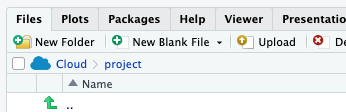
\includegraphics[width=0.5\textwidth,height=\textheight]{img/upload-to-posit-cloud.png}

}

\caption{\label{fig-upload-to-posit-cloud}}

\end{figure}%

Wählen Sie am besten den Ordner als Ziel, in dem sich auch die R-Datei,
von der aus Sie den Befehl zum Daten importieren schreiben, befindet.

\begin{tcolorbox}[enhanced jigsaw, coltitle=black, colframe=quarto-callout-note-color-frame, opacityback=0, toprule=.15mm, opacitybacktitle=0.6, arc=.35mm, titlerule=0mm, toptitle=1mm, title=\textcolor{quarto-callout-note-color}{\faInfo}\hspace{0.5em}{Note}, bottomtitle=1mm, leftrule=.75mm, breakable, rightrule=.15mm, colbacktitle=quarto-callout-note-color!10!white, bottomrule=.15mm, colback=white, left=2mm]

Es gibt verschiedene Formate, in denen (Tabellen-)Dateien in einem
Computer abgespeichert werden. Die gebräuchlichsten sind CSV und Excel.
Es gibt auch mehrere R-Befehle, um Daten in R zu importieren, z.B.
\texttt{read.csv()} oder \texttt{data\_read()}. Praktischerweise kann
der R-Befehl \texttt{data\_read()} viele verschiedene Formate
automatisch einlesen, so dass wir uns nicht weiter um das Format kümmern
brauchen. Der Vorteil von \texttt{read.csv} ist, dass Sie kein
Extra-Paket installiert bzw. gestartet haben müssen.

\end{tcolorbox}

\paragraph{Daten importieren per
Klick}\label{daten-importieren-per-klick}

RStudio Desktops GUI (Benutzeroberfläche) erlaubt es Ihnen auch, Daten
per Klick, also ohne R-Befehle, zu importieren, s.
Figure~\ref{fig-daten-rstudio}.

Sie können über diese Maske sowohl CSV-Dateien, Excel-Dateien oder
Daten-Dateien aus anderen Statistik-Programmen (z.B. SPSS) importieren
auf diese Weise.

Zur Erinnerung: CSV-Dateien sind Textdateien, wählen Sie in dem Fall
also \texttt{From\ Text}. Ich empfehle die Variante
\texttt{From\ Text\ (readr)\ ...}.

\begin{figure}

\centering{

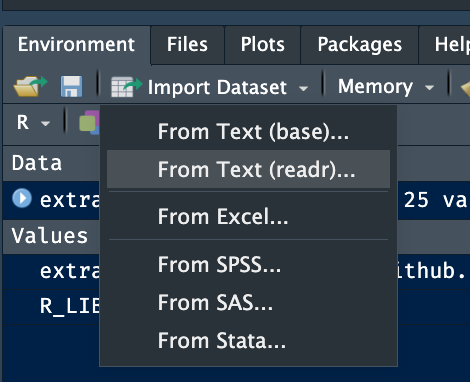
\includegraphics[width=0.5\textwidth,height=\textheight]{img/import-rstudio.png}

}

\caption{\label{fig-daten-rstudio}Daten importieren per Klick}

\end{figure}%

In der folgenden Maske können Sie unter \texttt{Browse} die zu
importierende Datendatei auswählen. Mit Klick auf \texttt{Import} wird
die Datei schließlich in R importiert.

\subsubsection{Dataframes}\label{dataframes}

Eine in R importierte Tabelle (mit bestimmten Eigenschaften) heißt
\emph{Dataframe}. Dataframes sind in der Datenanalyse von großer
Bedeutung.

\begin{definition}[Dataframe]\protect\hypertarget{def-dataframe}{}\label{def-dataframe}

Ein Dataframe (data frame; auch ``Tibble'' genannt\footnote{von ``tbl''
  wie Table}) ist ein Datenobjekt in R zur Darstellung von Tabellen.
Dataframes bestehen aus einer oder mehreren Spalten. Spalten haben einen
Namen, sozusagen einen ``Spaltenkopf''. Alle Spalten müssen die gleiche
Länge haben; anschaulich gesprochen ist eine Tabelle (in R) rechteckig.
Jede Spalte einzeln betrachtet kann als Vektor aufgefasst werden.
\(\square\)

\end{definition}

\textbf{?@tbl-mariokart} ist die Tabelle mit den Mariokart-Daten; etwas
präziser gesprochen ein Dataframe mit Namen \texttt{mariokart}. Übrigens
ist \textbf{?@tbl-mariokart} in Normalform (Tidy-Format), vgl.
\textbf{?@def-tidy}.

\begin{tcolorbox}[enhanced jigsaw, coltitle=black, colframe=quarto-callout-note-color-frame, opacityback=0, toprule=.15mm, opacitybacktitle=0.6, arc=.35mm, titlerule=0mm, toptitle=1mm, title=\textcolor{quarto-callout-note-color}{\faInfo}\hspace{0.5em}{Note}, bottomtitle=1mm, leftrule=.75mm, breakable, rightrule=.15mm, colbacktitle=quarto-callout-note-color!10!white, bottomrule=.15mm, colback=white, left=2mm]

Geben Sie den Namen eines Dataframes ein, um sich den Inhalt anzeigen zu
lassen. Beachten Sie, dass Sie die Daten auf diese Weise nur anschauen,
nicht ändern können. \(\square\)

\end{tcolorbox}

\subsubsection{Tabellen in R betrachten}\label{sec-viewtab}

Wenn Sie in R z.B. die Tabelle \texttt{mariokart} in einer
Excel-typischen Ansicht betrachten wollen, klicken Sie am besten auf das
Tabellen-Icon im Reiter \emph{Environment}, gleich neben dem Namen
\texttt{mariokart}, s. Figure~\ref{fig-view-mariokart}.

\begin{figure}

\centering{


\includegraphics[width=0.5\textwidth,height=\textheight]{img/rstudio-environment-mariokart.png}

}

\caption{\label{fig-view-mariokart}Per Klick auf das Tabellen-Icon
können Sie eine Tabellenansicht der Tabelle \texttt{mariokart} öffnen}

\end{figure}%

Alternativ öffnet der Befehl \texttt{View(mariokart)} die gleiche
Ansicht.

\subsection{Logikprüfung}\label{sec-logic}

\begin{quote}
Wer will schon wieder wen prüfen?!
\end{quote}

In diesem Abschnitt schauen wir uns \emph{Logikprüfungen} an: Wir lassen
R prüfen, ob eine Variable einen bestimmten Wert hat oder größer/kleiner
als ein Referenzwert ist.

Definieren wir zuerst eine Variable, \texttt{x}.

\begin{Shaded}
\begin{Highlighting}[]
\NormalTok{x }\OtherTok{\textless{}{-}} \DecValTok{42}
\end{Highlighting}
\end{Shaded}

Dann fragen wir R, ob diese Variable den Wert \texttt{42} hat.

\begin{Shaded}
\begin{Highlighting}[]
\NormalTok{x }\SpecialCharTok{==} \DecValTok{42}
\end{Highlighting}
\end{Shaded}

\begin{verbatim}
[1] TRUE
\end{verbatim}

\begin{quote}
Hallo, Mensch. Ja, diese Variable hat den Wert 42.
\end{quote}

(Danke, R.)

Möchte man mit R prüfen, ob eine Variable \texttt{x} einen bestimmten
\texttt{Wert} (``Inhalt'') hat, so schreibt man:

\texttt{x\ ==\ Wert}.

\begin{tcolorbox}[enhanced jigsaw, coltitle=black, colframe=quarto-callout-important-color-frame, opacityback=0, toprule=.15mm, opacitybacktitle=0.6, arc=.35mm, titlerule=0mm, toptitle=1mm, title=\textcolor{quarto-callout-important-color}{\faExclamation}\hspace{0.5em}{Important}, bottomtitle=1mm, leftrule=.75mm, breakable, rightrule=.15mm, colbacktitle=quarto-callout-important-color!10!white, bottomrule=.15mm, colback=white, left=2mm]

Man beachte das \emph{doppelte} Gleichheitszeichen. Zur Prüfung auf
Gleichheit muss man das doppelte Gleichheitszeichen verwenden.

\end{tcolorbox}

\begin{tcolorbox}[enhanced jigsaw, coltitle=black, colframe=quarto-callout-caution-color-frame, opacityback=0, toprule=.15mm, opacitybacktitle=0.6, arc=.35mm, titlerule=0mm, toptitle=1mm, title=\textcolor{quarto-callout-caution-color}{\faFire}\hspace{0.5em}{Caution}, bottomtitle=1mm, leftrule=.75mm, breakable, rightrule=.15mm, colbacktitle=quarto-callout-caution-color!10!white, bottomrule=.15mm, colback=white, left=2mm]

Ein beliebter Fehler ist es, bei der Prüfung auf Gleichheit, nur ein
Gleichheitszeichen zu verwenden, z.B. so: \texttt{x\ =\ 73}. Mit einem
Gleichheitszeichen prüft man aber \emph{nicht} auf Gleichheit, sondern
man definiert die Variable oder bestimmt ein Funktionsargument, s.
Section~\ref{sec-rvars}. \(\square\)

\end{tcolorbox}

Table~\ref{tbl-lgl} gibt einen Überblick über wichtige Logikprüfungen in
R.\footnote{Um das Zeichen für das logische ODER, \texttt{\textbar{}}
  auf einer Mac-Tastatur zu erhalten, drückt man \emph{Option+7}.}

\begin{longtable}{ll}

\caption{\label{tbl-lgl}Logische Prüfungen in R}

\tabularnewline

\toprule
Prüfung.auf & R-Syntax \\ 
\midrule\addlinespace[2.5pt]
Gleichheit & x == Wert \\ 
Ungleichheit & x != Wert \\ 
Größer als Wert & x > Wert \\ 
Größer oder gleich Wert & x >= Wert \\ 
Kleiner als Wert & x < Wert \\ 
Kleiner oder gleich Wert & x <= Wert \\ 
Logisches UND & (x < Wert1) \& (x > Wert2) \\ 
Logisches ODER & (x < Wert1) | (x > Wert2) \\ 
\bottomrule

\end{longtable}

\subsection{Praxisbezug}\label{praxisbezug}

\begin{quote}
🧑‍🎓Wird R in der Praxis wirklich genutzt? Oder ist R nur der Traum von
(vielleicht verwirrten) Profs im Elfenbeinturm?
\end{quote}

Schauen wir uns dazu die Suchanfragen bei
\href{www.stackoverflow.com}{stackoverflow.com} an, dem größten
FAQ-Forum für Software-Entwicklung. Wir vergleichen Suchanfragen mit dem
Tag \texttt{{[}r{]}} zu Suchanfragen mit dem Tag
\texttt{{[}spss{]}}\footnote{Durchgeführt am 2022-02-24, 17:21 CET}. Die
Ergebnisse sind in Abbildung Figure~\ref{fig-stackoverflow1}
dargestellt.

\begin{figure}

\centering{

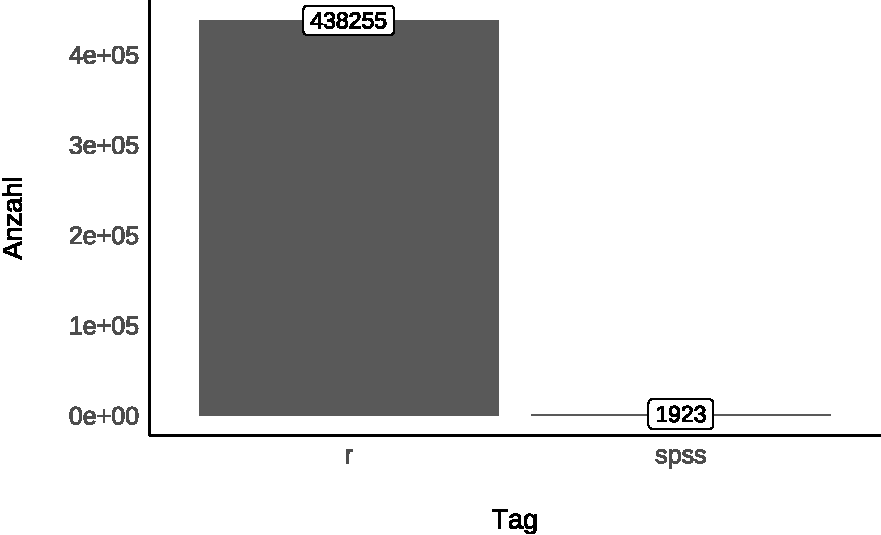
\includegraphics{020-R_files/figure-pdf/fig-stackoverflow1-1.pdf}

}

\caption{\label{fig-stackoverflow1}Suchanfragen nach R bzw SPSS, Stand
2022-02-24}

\end{figure}%

Das ist grob gerechnet ein Faktor von 200 (der Unterschied von R zu
SPSS). Dieses Ergebnis lässt darauf schließen, dass R in der Praxis viel
mehr als Excel gebraucht wird.

\begin{quote}
Aber ist R wirklich ein Werkzeug, das mir im Job hilft?
\end{quote}

Viele Firmen weltweit nutzen R zur Datenanalyse.\footnote{wie diese
  Liste zeigt:
  \url{https://www.quora.com/Which-organizations-use-R?share=1} zeigt}.

\begin{quote}
R ist \emph{der} Place-to-be für die Datenanalyse.
\end{quote}

\begin{quote}
Aber ist Datenanalyse wirklich etwas, womit ich in Zukunft einen guten
Job bekomme?
\end{quote}

Berufe mit Bezug zu Daten, Datenanalyse oder, allgemeiner, Künstlicher
Intelligenz (artificial intelligence) gehören zu den am meisten
wachsenden Berufen:

\begin{quote}
Artificial intelligence (AI) continues to make a strong showing on our
Emerging Jobs lists, which is no surprise. Many jobs that have risen up
as a result of AI in fields like cybersecurity and data science and
because it's is so pervasive many roles may demand more knowledge of AI
than you may think. For example, real estate and business development
roles. (Quelle: LinkedIn\footnote{\url{https://blog.linkedin.com/2019/december/10/the-jobs-of-tomorrow-linkedins-2020-emerging-jobs-report}})
\end{quote}

\subsection{Aufgaben}\label{aufgaben}

\begin{exercise}[Statistik-Meme]\protect\hypertarget{exr-meme}{}\label{exr-meme}

Suchen Sie ein schönes Meme zum Thema Statistik, Datenanalyse und Data
Science.
\href{https://data-se.netlify.app/2021/02/23/data-science-memes/}{Hier}
ist ein Startpunkt. \(\square\)

\end{exercise}

Die Webseite \href{https://datenwerk.netlify.app}{datenwerk.netlify.app}
stellt eine Reihe von einschlägigen Übungsaufgaben bereit. Sie können
die Suchfunktion der Webseite nutzen, um die Aufgaben mit den folgenden
Namen zu suchen:

\begin{enumerate}
\def\labelenumi{\arabic{enumi}.}
\tightlist
\item
  \href{https://datenwerk.netlify.app/posts/typ-fehler-r-01/typ-fehler-r-01.html}{Typ-Fehler-R-01}
\item
  \href{https://datenwerk.netlify.app/posts/typ-fehler-r-02/typ-fehler-r-02.html}{Typ-Fehler-R-02}
\item
  \href{https://datenwerk.netlify.app/posts/typ-fehler-r-03/typ-fehler-r-03.html}{Typ-Fehler-R-03}
\item
  \href{https://datenwerk.netlify.app/posts/typ-fehler-r-04/typ-fehler-r-04.html}{Typ-Fehler-R-04}
\item
  \href{https://datenwerk.netlify.app/posts/typ-fehler-r-06a/typ-fehler-r-06a.html}{Typ-Fehler-R-06a}
\item
  \href{https://datenwerk.netlify.app/posts/typ-fehler-r-07/typ-fehler-r-07.html}{Typ-Fehler-R-07}
\item
  \href{https://datenwerk.netlify.app/posts/typ-fehler-r-08-name-clash/typ-fehler-r-08-name-clash}{Typ-Fehler-R-08-name-clash}
\item
  \href{https://datenwerk.netlify.app/posts/logikpruefung1/logikpruefung1}{Logikpruefung1}
\item
  \href{https://datenwerk.netlify.app/posts/logikpruefung2/logikpruefung2}{Logikpruefung2}
\item
  \href{https://datenwerk.netlify.app/posts/there-is-no-package/there-is-no-package.html}{there-is-no-package}
\item
  \href{https://datenwerk.netlify.app/posts/wertberechnen2/wertberechnen2}{Wertberechnen2}
\item
  \href{https://datenwerk.netlify.app/posts/wertzuweisen_mc/wertzuweisen_mc}{Wertzuweisen\_mc}
\item
  \href{https://datenwerk.netlify.app/posts/argumente/argumente.html}{argumente}
\item
  \href{https://datenwerk.netlify.app/posts/import-mtcars/import-mtcars.html}{import-mtcars}
\item
  \href{https://datenwerk.netlify.app/posts/wertzuweisen/wertzuweisen}{Wertzuweisen}
\item
  \href{https://datenwerk.netlify.app/posts/wertpruefen/wertpruefen}{Wertpruefen}
\item
  \href{https://datenwerk.netlify.app/posts/wrangle1/wrangle1.html}{wrangle1}
\item
  \href{https://datenwerk.netlify.app/posts/repro1-sessioninfo/repro1-sessioninfo.html}{repro1-sessioninfo}
\item
  \href{https://datenwerk.netlify.app/posts/mw-berechnen/mw-berechnen}{mw-berechnen}
\end{enumerate}

Prüfen Sie Ihr Wissen mit
\href{https://datenwerk.netlify.app/posts/r-quiz/r-quiz}{diesem
Quiz}!\footnote{\url{https://datenwerk.netlify.app/posts/r-quiz/r-quiz}}

Noch nicht genug? Checken Sie alle Aufgaben mit dem Tag
\href{https://datenwerk.netlify.app/\#category=R}{R} auf dem Datenwerk
aus.\footnote{\url{https://datenwerk.netlify.app/\#category=R}}

\begin{tcolorbox}[enhanced jigsaw, coltitle=black, colframe=quarto-callout-note-color-frame, opacityback=0, toprule=.15mm, opacitybacktitle=0.6, arc=.35mm, titlerule=0mm, toptitle=1mm, title=\textcolor{quarto-callout-note-color}{\faInfo}\hspace{0.5em}{Note}, bottomtitle=1mm, leftrule=.75mm, breakable, rightrule=.15mm, colbacktitle=quarto-callout-note-color!10!white, bottomrule=.15mm, colback=white, left=2mm]

Die Webseite \href{https://datenwerk.netlify.app/}{Datenwerk} stellt
eine Reihe von Aufgaben zum Thema Statistik bereit. Zu jeder Aufgabe
sind ein oder mehrere Schlagwörter (Tags) zugeordnet. Wenn Sie auf ein
Schlagwort klicken, sehen Sie die Liste der Aufgaben mit diesem
Schlagwort. Es kann aber sein, dass Sie einige Aufgabe nicht lösen
können, da Wissen vorausgesetzt wird, das Sie (noch) nicht haben. Lassen
Sie sich davon nicht ins Boxhorn jagen. Ignorieren Sie solche Aufgaben
fürs Erste. \(\square\)

\end{tcolorbox}

\subsection{Vertiefung}\label{vertiefung-1}

\subsubsection{\texorpdfstring{Varianten zu
\texttt{read.csv}}{Varianten zu read.csv}}\label{varianten-zu-read.csv}

Hier ist eine weitere Möglichkeit, um Daten von einem Ordner (egal ob
dieser sich im Internet oder auf Ihrem Computer befinde) einzulesen,
stellt die Funktion \texttt{data\_read} bereit:

\begin{Shaded}
\begin{Highlighting}[]
\FunctionTok{library}\NormalTok{(easystats)  }\CommentTok{\# Das Paket muss installiert sein}
\NormalTok{d }\OtherTok{\textless{}{-}} \FunctionTok{data\_read}\NormalTok{(}\FunctionTok{paste0}\NormalTok{(}
  \StringTok{"https://vincentarelbundock.github.io/Rdatasets/"}\NormalTok{,}
  \StringTok{"csv/openintro/mariokart.csv"}\NormalTok{))}
\end{Highlighting}
\end{Shaded}

Der Unterschied ist, dass \texttt{data\_read} \emph{viele} Formate von
Daten (Excel, CSV, SPSS, \ldots) verkraftet, wohingegen
\texttt{read.csv} nur Standard-CSV einlesen kann.

Schauen wir uns die letzte R-Syntax en Detail an:

\begin{verbatim}
Hey R,
hol das "Buch" easystats aus der Bücherei und lies es
definiere als "d" die Tabelle,
die du unter der angegebenen URL findest.
\end{verbatim}

In R gibt es oft viele Möglichkeiten, ein Ziel zu erreichen. Zum
Beispiel haben wir hier den Befehl \texttt{data\_read()} verwendet, um
Daten zu importieren. Andere, gebräuchliche Befehle, die CSV-Dateien
importieren, heißen \texttt{read.csv()} (aus dem Standard-R, kein
Extra-Paket nötig) und \texttt{read\_csv()} (aus dem Meta-Paket
\texttt{\{tidyverse\}}).

\subsubsection{Importieren von
Excel-Tabellen}\label{importieren-von-excel-tabellen}

Mit der Funktion \texttt{data\_read} aus \texttt{\{easystats\}} kann man
viele verschiedene Datenformate importieren, auch Excel-Tabellen (.xls,
.xlsx).

Als Beispiel betrachten wir den Datensatz \texttt{extra} aus dem R-Paket
\texttt{\{pradadata\}}\footnote{\url{https://github.com/sebastiansauer/pradadata}}.
In diesem Datensatz werden die Ergebnisse einer Umfrage zu den
Korrelaten von Extraversion beschrieben. Details zu der
zugrundeliegenden Studie finden Sie hier: \url{https://osf.io/4kgzh}.

Ein Daten-Dictionary findet sich
\href{https://github.com/sebastiansauer/statistik1/raw/main/daten/extra-dictionary.md}{hier}.\footnote{\url{https://github.com/sebastiansauer/statistik1/raw/main/daten/extra-dictionary.md}}

Laden Sie die Excel-Datei herunter. Angenommen, Sie speichern die
Excel-Datei in einem Unterordner namens \texttt{daten} Ihres aktuellen
Projektordners. Dann können Sie die Daten so importieren:

\begin{Shaded}
\begin{Highlighting}[]
\FunctionTok{library}\NormalTok{(easystats)}
\end{Highlighting}
\end{Shaded}

\begin{verbatim}
# Attaching packages: easystats 0.7.1 (red = needs update)
x bayestestR  0.13.2    x correlation 0.8.4  
x datawizard  0.10.0    x effectsize  0.8.7  
x insight     0.19.10   x modelbased  0.8.7  
x performance 0.11.0    x parameters  0.21.6 
x report      0.5.8     
Restart the R-Session and update packages with `easystats::easystats_update()`.
\end{verbatim}

\begin{Shaded}
\begin{Highlighting}[]
\NormalTok{extra }\OtherTok{\textless{}{-}} \FunctionTok{data\_read}\NormalTok{(}\StringTok{"daten/extra.xls"}\NormalTok{)}
\end{Highlighting}
\end{Shaded}

\begin{verbatim}
Reading data...
\end{verbatim}

Allerdings kann \texttt{data\_read} keine Dateien aus dem Internet
importieren, was praktisch wäre. Stattdessen muss die Datei lokal auf
Ihrer Festplatte liegen.

Wenn Sie allerdings ``remote'', also aus dem Internet, eine Excel-Datei
importieren möchten, so können Sie das mit \texttt{import} aus dem
R-Paket \texttt{\{rio\}} tun:

\begin{Shaded}
\begin{Highlighting}[]
\FunctionTok{library}\NormalTok{(rio)}
\NormalTok{extra\_path }\OtherTok{\textless{}{-}} \FunctionTok{paste0}\NormalTok{(}
  \StringTok{"https://github.com/sebastiansauer/statistik1/"}\NormalTok{,}
  \StringTok{"raw/main/daten/extra.xls"}\NormalTok{)}
\NormalTok{extra }\OtherTok{\textless{}{-}} \FunctionTok{import}\NormalTok{(extra\_path)}
\end{Highlighting}
\end{Shaded}

\begin{tcolorbox}[enhanced jigsaw, coltitle=black, colframe=quarto-callout-note-color-frame, opacityback=0, toprule=.15mm, opacitybacktitle=0.6, arc=.35mm, titlerule=0mm, toptitle=1mm, title=\textcolor{quarto-callout-note-color}{\faInfo}\hspace{0.5em}{Note}, bottomtitle=1mm, leftrule=.75mm, breakable, rightrule=.15mm, colbacktitle=quarto-callout-note-color!10!white, bottomrule=.15mm, colback=white, left=2mm]

CSV-Dateien werden auf vielen Computern als eine Datei erkannt, die
Excel öffnen kann und das auch tut, wenn man eine CSV-Datei
doppelklickt. Dennoch ist das CSV-Format keine Datei im Excel-Format,
sondern eine einfache Text-Datei, die auch mit jedem Text-Editor
geöffnet und bearbeitet werden kann. \(\square\)

\end{tcolorbox}

Alternativ können Sie in RStudio auch Excel-Dateien \emph{ohne} R-Code
importieren, s. Figure~\ref{fig-daten-rstudio}.

\subsubsection{Der Dollar-Operator}\label{sec-dollar-op}

In Example~\ref{exm-vektoren} hatten wir Vektoren definiert. Solche
Vektoren fliegen sozusagen frei in Ihrem \texttt{Environment} herum
(Schauen Sie mal dort nach!) Die Spalten einer Tabelle sind aber auch
Vektoren, nur eben nicht frei im \texttt{Environment}, sondern in eine
Tabelle eingebunden.

Möchte man diese Vektoren direkt ansprechen, so kann man das mit dem
sog. \emph{Dollar-Operator} \texttt{\$} tun.

Angenommen, Sie möchten sich die Verkaufspreise (\texttt{total\_pr}) aus
der Tabelle \texttt{mariokart} herausziehen, dann können Sie das mit dem
Dollar-Operator tun:

\begin{Shaded}
\begin{Highlighting}[]
\NormalTok{mariokart}\SpecialCharTok{$}\NormalTok{total\_pr}
\end{Highlighting}
\end{Shaded}

\begin{verbatim}
  [1]  51.55  37.04  45.50  44.00  71.00  45.00  37.02  53.99  47.00  50.00
 [11]  54.99  56.01  48.00  56.00  43.33  46.00  46.71  46.00  55.99 326.51
 [21]  31.00  53.98  64.95  50.50  46.50  55.00  34.50  36.00  40.00  47.00
 [31]  43.00  31.00  41.99  49.49  41.00  44.78  47.00  44.00  63.99  53.76
 [41]  46.03  42.25  46.00  51.99  55.99  41.99  53.99  39.00  38.06  46.00
 [51]  59.88  28.98  36.00  51.99  43.95  32.00  40.06  48.00  36.00  31.00
 [61]  53.99  30.00  58.00  38.10 118.50  61.76  53.99  40.00  64.50  49.01
 [71]  47.00  40.10  41.50  56.00  64.95  49.00  48.00  38.00  45.00  41.95
 [81]  43.36  54.99  45.21  65.02  45.75  64.00  36.00  54.70  49.91  47.00
 [91]  43.00  35.99  54.49  46.00  31.06  55.60  40.10  52.59  44.00  38.26
[101]  51.00  48.99  66.44  63.50  42.00  47.00  55.00  33.01  53.76  46.00
[111]  43.00  42.55  52.50  57.50  75.00  48.92  45.99  40.05  45.00  50.00
[121]  49.75  47.00  56.00  41.00  46.00  34.99  49.00  61.00  62.89  46.00
[131]  64.95  36.99  44.00  41.35  37.00  58.98  39.00  40.70  39.51  52.00
[141]  47.70  38.76  54.51
\end{verbatim}

Der Dollar-Operator trennt den Namen der Tabelle vom Namen der Spalte.

Natürlich können Sie mit dem resultierenden Vektor beliebig
weiterarbeiten, etwa ihn in einem anderen Vektor speichern oder eine
Funktion anwenden:

\begin{Shaded}
\begin{Highlighting}[]
\NormalTok{verkaufspreise }\OtherTok{\textless{}{-}}\NormalTok{ mariokart}\SpecialCharTok{$}\NormalTok{total\_pr}
\FunctionTok{mean}\NormalTok{(verkaufspreise)}
\end{Highlighting}
\end{Shaded}

\begin{verbatim}
[1] 49.88049
\end{verbatim}

\begin{Shaded}
\begin{Highlighting}[]
\FunctionTok{mean}\NormalTok{(mariokart}\SpecialCharTok{$}\NormalTok{total\_pr)  }\CommentTok{\# synonym zur obigen Zeile}
\end{Highlighting}
\end{Shaded}

\begin{verbatim}
[1] 49.88049
\end{verbatim}

\subsubsection{R-Zertifikat bei
LinkedIn}\label{r-zertifikat-bei-linkedin}

Sie können bei LinkedIn\footnote{\url{https://www.linkedin.com/help/linkedin/answer/a510481}}
(oder anderen Anbietern ein Zertifikat) erhalten, das Ihre R-Kenntnisse
dokumentiert.

\subsubsection{R-Funktionen
verschachteln}\label{r-funktionen-verschachteln}

Das Kombinieren von Funktionen kann kompliziert werden:

\begin{codelisting}

\caption{\label{lst-schachtel}Verschachtelte Funktionen}

\centering{

\begin{Shaded}
\begin{Highlighting}[]
\NormalTok{x }\OtherTok{\textless{}{-}} \FunctionTok{c}\NormalTok{(}\DecValTok{1}\NormalTok{, }\DecValTok{2}\NormalTok{, }\DecValTok{3}\NormalTok{)}
\FunctionTok{sum}\NormalTok{(}\FunctionTok{abs}\NormalTok{(}\FunctionTok{mean}\NormalTok{(x)}\SpecialCharTok{{-}}\NormalTok{x)) }
\end{Highlighting}
\end{Shaded}

}

\end{codelisting}%

\begin{verbatim}
[1] 2
\end{verbatim}

Die Funktion \texttt{abs(x)} gibt den (Absolut-)Betrag von \texttt{x}
zurück (entfernt das Vorzeichen, mit anderen Worten).

Verschachtelte Ausdrücke lesen sich von innen nach außen (und werden in
dieser Reihenfolge abgearbeitet). Für unser Beispiel
(Listing~\ref{lst-schachtel}):

\begin{enumerate}
\def\labelenumi{\arabic{enumi}.}
\tightlist
\item
  Berechne den Mittelwert von \texttt{x}
\item
  Ziehe vom Mittelwert jeweils die Elemente von \texttt{x} ab
\item
  Nimm vom Ergebnis jeweils den Absolutwert
\item
  Summiere diese Werte
\end{enumerate}

Kurz gesagt: Hier haben wir die mittlere Absolutabweichung der Elemente
von \texttt{x} zum Mittelwert ausgerechnet.

\subsubsection{R und Friends updaten}\label{r-und-friends-updaten}

Irgendwann werden Ihr R, Ihr RStudio und Ihre R-Pakete veraltet sein, s.
Figure~\ref{fig-arnie}. Installieren Sie dann einfach die neue Version
von R und RStudio wie oben beschreiben, s. Section~\ref{sec-install-r}.

So updaten Sie Ihre R-Pakete: Klicken Sie im Reiter \texttt{Packages}
(in RStudio) und dort auf den Button \texttt{Update}.\footnote{Wenn die
  Anzahl der zu aktualisierenden Pakete groß ist, dann besser nicht alle
  auswählen, sondern nur ein paar. Dann die nächsten paar Pakete usw.}
Denken Sie daran, dass Sie die Software (R, RStudio, R-Paket), die Sie
updaten/installieren, nicht laufen darf.

\begin{tcolorbox}[enhanced jigsaw, coltitle=black, colframe=quarto-callout-note-color-frame, opacityback=0, toprule=.15mm, opacitybacktitle=0.6, arc=.35mm, titlerule=0mm, toptitle=1mm, title=\textcolor{quarto-callout-note-color}{\faInfo}\hspace{0.5em}{Note}, bottomtitle=1mm, leftrule=.75mm, breakable, rightrule=.15mm, colbacktitle=quarto-callout-note-color!10!white, bottomrule=.15mm, colback=white, left=2mm]

Ihre R-Pakete sollten aktuell sein. Klicken Sie beim Reiter
\emph{Packages} auf ``Update'', um Ihre R-Pakete zu aktualisieren.
Arnold Schwarzenegger rät, Ihre R-Pakete aktuell zu halten, s.
Figure~\ref{fig-arnie}\footnotemark{}.

\end{tcolorbox}

\footnotetext{Bildquelle: \url{https://imgflip.com/memegenerator}}

\begin{figure}

\centering{


\includegraphics[width=0.5\textwidth,height=\textheight]{img/terminator.jpg}

}

\caption{\label{fig-arnie}R-Pakete sollten stets aktuell sein, so Arnold
Schwarzenegger}

\end{figure}%

\subsubsection{Benötigte R-Pakete}\label{benuxf6tigte-r-pakete}

In diesem Kapitel benötigen Sie folgendes R-Paket:

\begin{Shaded}
\begin{Highlighting}[]
\FunctionTok{library}\NormalTok{(openintro)  }\CommentTok{\# Datensatz \textasciigrave{}mariokart\textasciigrave{}}
\end{Highlighting}
\end{Shaded}

\begin{verbatim}
Loading required package: airports
\end{verbatim}

\begin{verbatim}
Loading required package: cherryblossom
\end{verbatim}

\begin{verbatim}
Loading required package: usdata
\end{verbatim}

\begin{verbatim}

Attaching package: 'openintro'
\end{verbatim}

\begin{verbatim}
The following object is masked from 'package:gt':

    sp500
\end{verbatim}

\subsubsection{Benötigte Daten}\label{benuxf6tigte-daten}

Sie benötigen in diesem Kapitel den Datensatz \texttt{mariokart}, der
entweder online\footnote{ über diese Internetadresse:
  \url{https://vincentarelbundock.github.io/Rdatasets/csv/openintro/mariokart.csv}}
oder über R-Paket \texttt{openintro} importiert werden kann:

\paragraph{Import via Download}\label{import-via-download}

\begin{Shaded}
\begin{Highlighting}[]
\NormalTok{mariokart }\OtherTok{\textless{}{-}} \FunctionTok{read.csv}\NormalTok{(}\FunctionTok{paste0}\NormalTok{(}
  \StringTok{"https://vincentarelbundock.github.io/Rdatasets/"}\NormalTok{,}
  \StringTok{"csv/openintro/mariokart.csv"}\NormalTok{))}
\end{Highlighting}
\end{Shaded}

\paragraph{Import via R-Paket}\label{import-via-r-paket}

\begin{Shaded}
\begin{Highlighting}[]
\CommentTok{\# Das Paket \textquotesingle{}openintro\textquotesingle{} muss installiert sein:}
\FunctionTok{data}\NormalTok{(mariokart, }\AttributeTok{package =} \StringTok{"openintro"}\NormalTok{) }
\end{Highlighting}
\end{Shaded}

\subsection{Literaturhinweise}\label{literaturhinweise}

``Warum R? Warum, R?'' heißt ein Kapitel in @sauer\_moderne\_2019, das
einiges zum Pro und Contra von R ausführt. In Kapitel 3 in der gleichen
Quelle finden sich viele Hinweise, wie man R startet; In Kapitel 4
werden Grundlagen von ``Errisch'' erläutert; Kapitel 5 führt in
Datenstrukturen von R ein (schon etwas anspruchsvoller). Alternativ
bietet \href{https://moderndive.com/1-getting-started.html}{Kapitel 1}
von @ismay\_statistical\_2020 einen guten und sehr anwenderfreundlichen
Überblick. Das Buch hat auch den Vorteil, dass es komplett frei online
verfügbar ist. Vergleichbar dazu ist
@cetinkaya-rundel\_introduction\_2021, vielleicht einen Tick formaler;
auf jeden Fall genau das richtige Niveau für Bachelor-Statistik in
angewandten nicht-technischen Studiengängen.

Natürlich gibt es viele Online-Kurse zu R, die aber teilweise
kostenplichtig sind\footnote{Ein Beispiel ist der Kurs \emph{Getting
  Started with RStudio},
  \url{https://www.coursera.org/projects/getting-started-rstudio}
  (Kursdauer: 1 Stunde)}.

\subsection{Literatur}\label{literatur}




\end{document}
